%% <UTF-8>
%% 北京航空航天大学学位论文模板版主文件
%% 编译方式：XeLaTeX 连续编译 2-3 次。

\documentclass[doctor,public,oneside,win]{buaa}

\refcolor{off}
\beginright{on}
\emptypagewords{}

% 额外宏包。buaa.cls 已包含 graphicx、float、booktabs、longtable、amsmath 等常用包。
\usepackage{amssymb}
\usepackage{colortbl}
\definecolor{lightgray}{gray}{0.84}

% 论文题目-{中文}{英文}
\Title{基于视觉语言大模型的医学病理图像无监督检测和分割方法研究}
{Research on Unsupervised Detection and Segmentation Methods for Medical Pathology Images Based on Vision-Language Large Models}

% 学科、院系、专业和研究方向。若学校最终口径不同，优先在这里修改。
\Branch{工学}
\Department{生物科学与医学工程学院}
\Major{生物医学工程}
\Feild{医学图像分析与数字病理}

% 导师与学生信息。英文名和具体职称可后续按学院要求再精修。
\Tutor{许燕}{Yan Xu}{教授}
\Author{吴永健}{Yongjian Wu}
\StudentID{BY2110209}

% 中图分类号可后续按最终学科方向调整。
\CLC{TP391.4}

% 时间节点-{月}{日}{年}，这里先给可编译占位值。
\DateEnroll{09}{01}{2021}
\DateGraduate{06}{30}{2026}
\DateSubmit{06}{14}{2026}
\DateDefence{06}{30}{2026}

% 摘要-{中文}{英文}
\Abstract{%
医学病理图像的目标检测与实例分割是数字病理分析、疗效评估和临床辅助决策的重要基础。然而，病理图像具有目标密集、形态差异细微、跨中心染色与扫描风格差异显著等特点，高质量框标注与实例级标注获取成本高，长期制约了相关方法在开放类别与跨域场景中的可扩展性与泛化能力。围绕上述瓶颈，本文以“尽量减少对昂贵标注的依赖，同时增强模型在开放类别与跨域场景中的泛化能力”为总体目标，面向视觉语言大模型的提示学习机制，系统研究无/弱监督条件下的病理图像检测、分割与数字病理量化方法。

本文首先研究在缺乏目标域检测标注时如何建立可用的细胞核检测入口，提出基于自动属性提示与自训练的零样本细胞核检测方法，通过自动构造医学属性描述并结合目标域自适配，降低对人工检测标注与手工提示模板的依赖。其次，针对病理域中零样本检测对提示工程的敏感性以及密集细胞核易漏检、重叠的问题，提出自动提示框架 AttriPrompter：从无标注病理图像中自动生成形状/颜色属性，并通过同义与“程度”增强扩展描述粒度，进一步按图文相关性对提示序列进行排序以驱动视觉语言检测器获得更稳定的初始定位；在此基础上，引入自训练知识蒸馏迭代优化，以伪标签促进目标域适配并提升无监督检测性能。再次，针对纯文本提示难以稳定表达细粒度视觉差异的问题，提出视觉文本化方法，将少量支持图像映射为语言空间兼容的提示表示，从而以图像提示增强开放词汇感知与跨域推理能力。最后，本文将前述识别能力迁移到临床问题中，构建面向肺鳞癌新辅助免疫化疗后疗效评估的数字病理分析框架，联合量化残余肿瘤负荷和肿瘤周围免疫细胞密度，为疗效评估与预后分析提供辅助信息。

从研究主线看，本文的四项工作体现了从“提示驱动的识别能力构建”到“临床导向的可解释量化”的逐步推进：先以自动属性提示与自训练建立目标域检测入口，再以 AttriPrompter 的“属性生成—增强—排序”自动提示机制与自训练蒸馏提升零样本检测质量与域适配能力，继而以图像提示的视觉文本化机制增强跨域感知，最终将方法落地到具有临床解释价值的数字病理分析任务中。相关研究表明，视觉语言大模型与提示学习为降低病理图像任务标注成本、提升开放场景泛化能力提供了一条具有潜力的技术路线。
}{%
Medical image detection and segmentation are fundamental tasks in medical artificial intelligence and serve as essential prerequisites for digital pathology analysis, treatment assessment, and clinical decision support. However, progress in this area is constrained by the high cost of dense annotation, severe domain shifts across institutions and staining protocols, and the difficulty of describing fine-grained medical targets using simple category labels. To address these challenges, this thesis studies unsupervised and weakly supervised medical image detection, segmentation, and digital pathology analysis with the overarching goal of reducing annotation dependence while improving generalization under open-vocabulary and cross-domain settings.

First, this thesis studies how to establish a practical nuclei detection entry point without target-domain detection annotations, and proposes a zero-shot nuclei detection framework based on automatic attribute prompting and self-training, which reduces dependence on manual detection labels and hand-crafted medical prompt templates. Second, to mitigate the sensitivity of zero-shot pathology detection to prompt engineering and address missed/overlapped detections in dense nuclei scenes, this thesis proposes an auto-prompting framework, AttriPrompter, which automatically generates shape/color attributes from unlabeled pathology images, enriches them with synonym and degree-based expansions, and ranks prompt sequences by image–text relevance to produce more reliable initial grounding; furthermore, a self-trained knowledge distillation scheme is introduced to iteratively improve pseudo labels and enhance target-domain adaptation for unsupervised nuclei detection. Third, to overcome the limitation of purely textual prompts in representing subtle visual differences, a visual textualization framework is proposed, which maps a small number of support images into language-space-compatible prompt representations and enables image-prompted detection and segmentation with improved cross-domain perception. Finally, the developed recognition capability is applied to a clinically oriented digital pathology problem, namely AI-based assessment of tumor regression and peritumoral immune cell density for treatment evaluation and prognosis analysis in lung squamous cell carcinoma after neoadjuvant immunochemotherapy.

Taken together, the four studies form a coherent research trajectory from prompt-driven recognition capability construction to clinically interpretable digital pathology quantification. The results suggest that vision-language large models and prompt learning provide a promising pathway for reducing annotation cost and improving generalization in computational pathology.
}

% 关键字-{中文}{英文}
\Keyword{医学图像分析，细胞核检测，实例分割，视觉语言预训练，提示学习，数字病理}
{medical image analysis, nuclei detection, instance segmentation, vision-language pre-training, prompt learning, digital pathology}

% 图表目录
\Listfigtab{on}

% 主要符号表/缩写表
% TODO: 这里原来用了 tabular，当前触发编译报错（\\ 与间距环境冲突）。先临时置空，待全文编译恢复后再补回。
\Abbreviations{}

\begin{document}

% 正文。摘要由 buaa 模板自动生成，因此不再输入 chapters/00_abstract.tex。
\chapter{绪论}

\section{研究背景}
医学图像检测、分割与量化分析是医学人工智能研究中的核心内容。对于病理图像而言，细胞核检测与实例分割直接关系到组织结构理解、细胞计数、肿瘤微环境分析和后续临床量化建模；对于放射与病理融合分析而言，可靠的区域定位和结构提取又是疗效评估、风险分层和预后预测的重要基础。可以说，前端识别能力的稳定性在很大程度上决定了后续医学分析任务的上限。

然而，这一领域长期存在两个互相交织的难题。其一是监督信号昂贵且稀缺。医学图像尤其是病理图像中的实例级标注，需要专业病理医师或经过长期训练的研究人员完成，时间成本与经济成本都很高。其二是目标域迁移困难。同一疾病在不同中心、不同切片制备流程、不同染色和不同扫描仪条件下，会表现出明显不同的数据分布；即使模型在单一公开数据集上表现良好，一旦进入真实场景，也常常面临性能下降的问题。

近年来，大规模视觉语言预训练模型的兴起为解决上述问题提供了新的可能。一方面，这类模型具备一定的开放词汇识别能力，使得“未见类别识别”和“少样本适配”不再完全依赖人工标注；另一方面，提示学习机制使模型有机会在结构保持相对稳定的前提下，通过较少附加参数实现目标域迁移。这些新进展为医学图像分析带来了新的方法论转向，即从传统强监督闭集学习逐步走向弱监督、无监督和开放场景建模。

\section{研究动机}
本文的研究动机来源于一个持续演化的认识：虽然医学图像强监督标注昂贵，但目标结构、跨模态知识以及少量示例本身蕴含着可被模型利用的先验。换言之，昂贵人工标注并不是唯一的监督来源，合理设计的伪标签、自训练、文本提示、图像提示和结构先验都可能成为替代性学习信号。

沿着这一思路，本文将研究问题组织为一条从“识别入口构建”走向“临床量化解释”的主线：首先，在缺乏目标域检测标注时，如何借助视觉语言大模型的开放词汇能力与自动提示构造建立零样本细胞核检测入口？其次，当零样本病理检测对手工提示工程高度敏感、且密集细胞核易出现漏检与重叠时，如何通过自动提示机制生成更稳定的语义入口，并结合自训练迭代实现目标域适配？再次，当纯文本提示难以稳定表达细粒度医学视觉差异时，如何进一步让图像提示以兼容形式进入视觉语言模型，以增强跨域感知与推理能力？最后，当前端识别能力逐步建立后，如何将其组织为可解释、可统计的数字病理指标，用于疗效评估与预后分析？

\section{研究内容}
围绕上述主线，本文主要开展以下四方面研究。

第一，研究视觉语言大模型在细胞核检测中的迁移问题，提出基于自动属性提示与自训练的零样本细胞核检测方法。该工作解决的是“缺乏目标域检测标注时如何构造可辨识的医学提示，并将开放词汇能力转化为目标域可用的检测性能”。

第二，针对零样本检测对提示工程的敏感性以及密集细胞核场景下的漏检、重叠问题，提出自动提示框架 AttriPrompter：从无标注病理图像中自动生成形状/颜色属性，并通过同义与“程度”增强扩展描述粒度，进一步按图文相关性对提示序列排序以获得更可靠的初始定位；在此基础上，引入自训练知识蒸馏迭代优化，以伪标签驱动目标域适配并提升无监督检测性能。该工作解决的是“如何在无需人工提示模板与检测标注的条件下，自动构造高质量提示并稳定提升零样本检测效果”。

第三，研究图像提示与文本提示的统一建模与注入机制，提出视觉文本化方法，通过将少量支持图像映射到语言空间兼容的提示表示，增强模型对细粒度差异与跨域风格变化的感知能力。该工作解决的是“当文本描述不足时，如何让图像示例以提示的形式直接参与推理”。

第四，将上述方法体系进一步应用于肺鳞癌新辅助免疫化疗后的数字病理分析，构建面向残余肿瘤负荷与肿瘤周围免疫细胞密度的量化框架，并通过统计分析探索其与疗效及预后之间的关系。该工作解决的是“如何将检测、分割结果转化为临床可解释指标并形成分析闭环”。

\section{技术路线}
本文的技术路线可以概括为“从提示驱动的识别能力构建到临床导向的可解释量化”的逐步推进：前期工作面向无检测标注场景，重点解决自动提示构造与目标域自适配问题；中期工作进一步面向未见类别与跨域分布偏移，重点解决结构先验注入与提示融合问题；后期工作将上述识别能力整合到临床导向的数字病理链条中，强调可解释指标构建与统计验证。

从建模角度看，本文的方法体系有三个共同特点。第一，强调尽量减少对昂贵强监督标注的依赖。第二，强调最大化利用视觉语言预训练带来的跨模态先验，并通过提示机制进行轻量适配。第三，强调输出结果的可解释性，使方法不仅服务于 benchmark 指标，也服务于真实数字病理分析需求。

\section{论文结构安排}
全文共分七章。第一章为绪论，介绍研究背景、动机、内容和结构安排。第二章总结相关研究基础，包括视觉语言预训练、提示学习、医学检测与分割以及数字病理分析。第三章介绍自动属性提示与自训练联合的零样本细胞核检测方法。第四章介绍自动提示框架 AttriPrompter 及其自训练知识蒸馏的迭代优化方法。第五章介绍视觉文本化框架及其图像提示驱动的检测与分割方法。第六章介绍面向肺鳞癌疗效评估的数字病理量化分析框架。第七章对全文进行总结并讨论后续研究方向。

\section{主要贡献}
本文的主要贡献体现在以下四个方面。其一，提出了基于自动属性提示与自训练的零样本细胞核检测方法，为医学无标注检测提供了可扩展的实现路径。其二，提出了自动提示框架 AttriPrompter，通过“属性生成—增强—排序”自动构造高质量提示序列，并结合自训练知识蒸馏提升密集细胞核场景下的零样本检测稳定性与目标域适配能力。其三，提出了视觉文本化方法，将图像提示映射到语言空间，从而增强模型在跨域与细粒度目标场景中的感知能力。其四，构建了面向肺鳞癌疗效评估的数字病理分析框架，将前端识别结果进一步组织为具有临床解释意义的量化指标并开展统计分析。

\chapter{相关研究基础}

\section{医学图像检测与分割研究的总体脉络}
医学图像分析的发展大体经历了从手工特征、浅层机器学习到深度学习，再到预训练大模型和提示学习的几个阶段。早期方法主要依赖阈值分割、区域生长、活动轮廓模型、形态学算子以及人工设计纹理特征来完成病灶或组织结构提取。这类方法的优点是可解释性强、实现简单，但它们通常只能适用于成像条件较为稳定、目标形态变化较小的任务。一旦遇到病理染色变化、扫描噪声增强或者目标边界模糊等问题，传统方法往往很难保持稳定性能。

随着卷积神经网络的成功应用，医学图像分析逐渐进入深度学习阶段。以 U-Net 为代表的编码器--解码器结构推动了像素级分割任务的快速发展，Mask R-CNN 及其变体则推动了实例级分割的发展。对于细胞核检测与分割任务而言，深度学习方法显著提高了边界恢复能力和复杂背景下的识别能力。然而，这一阶段的方法几乎都建立在“存在足够强监督标注”的前提之上，也因此把问题转移到了数据构建成本上。医学数据的标注瓶颈并没有因为模型变强而消失，反而由于模型更依赖大规模训练而变得更加突出。

近几年，视觉语言预训练和基础模型的发展又把医学图像分析推入新的阶段。研究重点开始从“如何在固定数据集上逼近最优精度”转向“如何减少对强监督标注的依赖”“如何在开放类别和跨域场景中泛化”以及“如何利用文本、图像示例和外部知识协助推理”。本文所关注的弱监督、零样本、图像提示和数字病理分析问题，本质上都处在这一新阶段的演进链条中。

\section{弱监督与无监督医学图像分割}

\subsection{弱监督分割的基本思想}
弱监督分割的基本目标是利用比像素级标注更廉价的监督信息近似恢复目标区域。常见弱监督信号包括图像级标签、点标注、框标注、涂鸦标注以及部分伪标签。不同监督形式对应不同的信息上限：图像级标签最廉价，但只告诉模型某类目标是否存在；点和框能提供更明确的空间约束，但边界信息仍然缺失；涂鸦比点和框更接近真实轮廓，但人工成本也更高。如何在“监督强度”和“标注成本”之间取得平衡，是弱监督分割长期关注的问题。

在自然图像领域，类激活图、区域提案、条件随机场后处理和自训练策略构成了图像级弱监督分割的主流技术路线。即先通过分类网络获得目标的粗激活分布，再利用后处理或迭代优化方式把粗热图转化为较完整的掩码。在医学图像场景中，这一思路同样具有启发性，但直接照搬并不总是有效。医学对象尤其是细胞核目标具有尺度小、密度高、粘连严重等特点，使得自然图像中的弱监督前景恢复策略很难直接实现高质量实例边界提取。

\subsection{病理图像中的特殊困难}
病理图像弱监督分割面临的困难具有鲜明的结构性。首先，细胞核等目标往往尺寸小、数量多，相互之间距离很近，一旦伪标签稍微膨胀，就会把多个目标错误地连在一起。其次，病理图像中的颜色和纹理受染色和扫描条件影响显著，不同样本之间的成像风格变化容易导致弱监督定位结果不稳定。再次，病理图像中存在大量与目标外观接近的背景结构，这些结构往往会在弱监督阶段被错误激活，造成伪标签污染。

因此，病理图像中的弱监督分割方法通常不能只停留在“恢复前景区域”层面，而必须进一步思考如何形成实例级结构感知。这也是为什么细胞核分割工作中常常会显式引入边界分支、距离变换分支或中心点约束等结构先验。类似地，本文后续针对密集细胞核场景中的漏检与重叠问题，也引入了基于伪标签迭代的自训练/蒸馏机制，以在弱监督信号有限的条件下逐步提升结构化定位质量。

\subsection{伪标签与自训练}
伪标签和自训练在弱监督与半监督分割中占据重要位置。其基本思想是先利用现有模型生成高置信预测，再把这些预测当作新监督信号继续训练模型。成功的关键在于：伪标签既不能过于保守，否则覆盖率不足；也不能过于激进，否则错误会在迭代中不断放大。在医学图像中，这个平衡更难把握，因为目标形态复杂且域偏移明显。

已有研究证明，自训练在医学图像中并非简单的“多跑几轮”策略，而需要与结构先验、分支解耦或多任务约束结合。对于本文的研究主线而言，伪标签与自训练并不是一个孤立技术点，而是一种贯穿多篇工作的核心思想：从弱监督分割中的伪标签迭代优化，到零样本检测后的目标域自适配（自训练/蒸馏），再到图像提示学习中的少样本引导，都能看到“先构造一个可接受起点，再通过数据反馈逐步提升”的共通逻辑。

\section{细胞核检测与实例分割研究}

\subsection{检测、分割与联合建模}
细胞核分析任务通常分为三类：核检测、语义分割和实例分割。核检测强调目标位置，适合计数和密度估计；语义分割强调前景区域覆盖，适合估计总体核面积；实例分割则要求区分每个独立核目标，最适合后续的形态统计和组织微环境分析。三类任务并非彼此割裂，而是存在显著内在联系。一个好的实例分割模型往往隐含具有检测能力，一个好的检测器也通常能为实例学习提供较稳定候选区域。

在病理图像中，许多方法试图将检测与分割联合建模。例如，有的工作先进行核中心点检测，再以中心点为引导恢复边界；有的工作同时预测前景图、边界图和距离图，以实现实例拆分；还有的工作直接通过 proposal-based 结构完成实例掩码预测。不同方法的差异在于对实例结构的建模方式不同，但它们都说明一件事：对于高密度细胞核任务，仅靠单一前景预测往往不够，必须引入额外结构信息。

\subsection{跨数据集与跨域问题}
细胞核数据集之间的差异很大。不同组织来源、不同切片质量、不同染色方案和不同扫描仪都会导致目标外观变化。一个在单一公开 benchmark 上表现优异的模型，进入真实跨域场景后往往会遇到性能下降。因此，单纯追求单数据集分数并不足以说明方法的实用性。如何在有限目标域支持样本甚至无支持样本条件下增强泛化能力，已经成为细胞核分析研究的重要方向。

这一点与本文后续关于跨域评测（domain shift）、少样本支持提示（few-shot prompting）以及“冻结主干、仅通过提示适配”的直测设定密切相关。作者之所以反复强调源域训练、目标域少量支持样本提示与不进行目标域大规模微调，是因为细胞核分析任务的实际挑战并不仅仅是“在一个数据集上做得更高”，而是“面对新域时还能否工作”。从学位论文角度看，这种问题意识也使得全文研究比单纯追求基准分数更具完整性。

\section{视觉语言预训练模型及其医学迁移}

\subsection{视觉语言预训练的基本范式}
视觉语言预训练模型通过大规模图文对构建跨模态共享语义空间。CLIP 通过图像编码器和文本编码器的对比学习训练获得强分类迁移能力，BLIP 在此基础上进一步增强生成与理解能力，而 GLIP 则尝试把语言提示直接融入目标检测框架，使检测器具备开放词汇识别能力。这一系列模型的重要意义在于，它们使图像理解不再局限于固定类别表，而可以借助文本描述扩展到未见对象。

在自然图像领域，开放词汇检测的价值已经得到广泛验证。但在医学图像领域，这一能力并不能直接迁移。首先，医学图像的许多概念在大规模通用图文语料中本来就稀缺；其次，医学对象往往依赖局部结构模式而非简单语义标签；再次，医学任务常常需要非常稳定的定位能力，而非仅仅粗粒度识别。因此，视觉语言模型迁移到医学场景时，需要配合新的提示机制、目标域自适应机制和可能的结构先验。

\subsection{开放词汇与零样本能力的局限}
尽管视觉语言模型具备开放词汇能力，但在医学任务中，单靠文本类名通常不足以支撑高质量检测。例如，同样是“细胞核”，不同病理环境下的核在大小、形状、染色情况和周边背景方面可能完全不同。简单提示无法表达这种差异，甚至会导致模型偏向自然图像语义空间中的错误对象。因此，零样本医学检测如果要真正成立，必须在提示构造和目标域适配上做更细致设计。

本文第三章正是在这一局限之上提出自动属性提示构造。其出发点不是否认视觉语言模型的价值，而是承认“医学类别语义不足”的现实，然后试图以属性、描述和自训练的方式弥补这一不足。从相关工作回顾角度看，这使得本文不是简单使用现成大模型，而是在其基础上提出新的迁移方法。

\section{提示学习的发展与图像提示研究}

\subsection{文本提示学习}
提示学习最早主要体现为对文本模板的设计。研究者通过改变 prompt phrasing 来影响模型对类别的理解，例如“a photo of a dog”和“this is a dog”在 CLIP 类模型中可能带来不同效果。随着研究发展，更多工作开始引入可学习 prompt token，以代替人工设计模板。对医学图像而言，文本提示学习具有明显吸引力，因为它不需要大规模改动模型结构，却可以借助预训练语义进行目标域适配。

不过，医学场景中的文本提示存在两个根本局限。第一，语言本身未必能精确表达细粒度视觉差异。第二，许多医学任务对形态和组织结构极为敏感，而这些信息天然更容易通过视觉示例表达，而非通过词语表达。因此，仅依赖文本 prompt 往往不足以满足复杂医学场景需求。

\subsection{图像提示与多模态提示}
图像提示的核心思想是让支持图像本身参与推理，以补充纯文本提示不足。已有工作在通用目标检测、分割和 few-shot 学习中表明，少量支持样本可以显著改善模型对新类别的感知能力。但如何让图像提示与原有视觉语言预训练结构兼容，仍是一个开放问题。若处理不当，图像提示可能破坏原有图文对齐能力，导致模型难以稳定收敛。

在医学场景下，图像提示的潜力更加明显。一个病理专家往往只需要看几张代表性示例就能理解某类目标的大致外观，而图像提示恰好模拟了这种“示例式知识传递”过程。本文第五章的视觉文本化工作，就是对这一思路的系统展开：既不放弃文本提示提供的语义框架，又引入图像提示补充细粒度结构信息。

\section{数字病理分析与可解释医学人工智能}

\subsection{从识别到量化}
数字病理研究正在从“自动识别病灶”向“自动量化病理表型”演化。前者关注的是目标是否被正确找出，后者关注的是目标识别后能否形成对医生有意义的统计指标。例如，肿瘤残留比例、免疫细胞密度、肿瘤边界结构变化以及细胞空间共定位模式，都属于后者关心的内容。

这种演化意味着，前端检测和分割结果的意义不再只体现为 benchmark 分数，而是要进一步考虑结果是否足以支持后续统计分析与临床解释。因此，一个看似精度很高但结构不稳定的模型，未必真的适合数字病理分析；相反，一个在临床关键指标上更稳定、更可解释的模型，可能更有实际应用价值。

\subsection{临床结局建模}
在肿瘤研究中，治疗后病理切片提供了非常丰富的预后信息。除了传统的病理缓解程度评估，肿瘤周围免疫细胞的数量、密度和空间分布也逐渐被认为与治疗反应和生存结局有关。AI 模型若能稳定识别并量化这些指标，就能为更细致的风险分层和个体化治疗提供辅助。

本文第六章的肺鳞癌工作正是建立在这一思想之上。它使得前几章偏方法论的研究，有了一个自然的应用收束点，也让整篇学位论文的价值不局限于算法创新，而延伸到临床解释和数字病理转化。

\section{本章小结}
本章系统回顾了本文后续研究所依赖的相关基础，包括弱监督与无监督医学分割、细胞核检测与实例分割、视觉语言预训练模型、提示学习以及数字病理分析。从这些工作的发展脉络可以看到，本文四项研究并不是偶然拼接，而是分别对应“监督不足”“语义不足”“跨域适配”和“临床解释”四类连续问题。基于这一认识，后续章节将依次展开具体方法与实验分析。

% 工作一：Zero-shot nuclei detection
\chapter{基于自动属性提示的零样本细胞核检测}

\section{研究背景}
在医学图像处理领域，苏木精和曙红（H＆E）染色图像的细胞核检测在生物医学研究和临床应用的各个领域中发挥着至关重要的作用\cite{gleason1992histologic}。进行像素级实例掩码的标注工作是极其费时费力的，需要医生重复标注大量细胞，并且由于细胞核往往密集和微小，比自然图像或者其他类型的医学图像数据集（比如眼底，骨骼，器官组织等）更加难以标注。像素级实例掩码还要求更精确的轮廓，相比之下，在传统细胞核检测场景中，模型如果依赖大量边界框或点级标注进行训练能相对降低标注成本，但在真实病理研究中，构建多数据集、多中心和多类别核检测标注依然代价高昂。尤其是在研究新组织类型、稀有类别或跨域迁移问题时，检测标注往往成为限制模型快速拓展的重要瓶颈。总之无论是采用何种形式的标注，其标注准备工作的繁杂程度都是难以承受的，极大得阻碍了相关的科学研究和技术应用。具体来说，比如\cite{mahanta2021ihc,graham2019hover,yi2019multi}等方法提出了完全监督的有效方法，但由于标注工作仍然是劳动密集型且昂贵的，现实应用中依然困难重重。

为了解决上述问题，人们提出了几种无监督方法，包括基于阈值保持的方法\cite{jiao2006improved,mouelhi2018fast}、基于自监督的方法\cite{sahasrabudhe2020self}和基于领域适应的方法\cite{le2022unsupervised}。其中，域适应方法是主流，通过对齐源域和目标域来实现适应，并表现出良好的性能\cite{le2022unsupervised}。然而，当前的无监督方法表现出较强的经验设计，使得在模型设计过程中引入了主观偏差，因此当前的无监督方法可能会导致次优结果。然而，新开发的大规模视觉语言预训练模型（VLPM）提供了另一种可能的无监督学习范式\cite{radford2021learning,jia2021scaling}。 VLPM 从互联网上获取的大量文本图像对中学习对齐的文本和图像特征，使学习到的视觉特征语义丰富、通用且可转移。基于VLPM的零样本学习方法用于文本驱动的图像处理\cite{patashnik2021styleclip}、图像字幕\cite{li2022blip}、视图合成\cite{jain2021putting}和目标检测\cite{li2022grounded}等下游任务，取得了优异的结果。在 VLPM 中，在对象级别进行预训练的基础语言图像预训练（GLIP）模型 \cite{li2022grounded} 甚至可以在零样本对象检测和短语基础任务中与完全监督的模型相媲美。尽管 VLPM 已被用于自然场景中的物体检测，但通过 VLPM 对 H\&E 图像进行零样本核检测仍然没有得到充分探索。医学 H\&E 图像与用于预训练的自然图像之间的显着域差异使得这项任务具有挑战性。人们想知道VLPM是否可以凭借其丰富的语义信息，通过语义驱动的提示来直接预测细胞核检测，建立一个优雅、简洁、清晰但更高效和可移植的无监督系统，用于无标记细胞核检测。基于这个概念，我们的目标是建立一个基于 VLPM 的零样本核检测框架。然而，直接应用 VLPM 来完成这项任务会带来两个挑战。 （1）由于医学图像和用于预训练的网络源文本图像对之间存在差距，文本编码器可能缺乏医学概念词的先验知识，从而使零样本检测的提示设计成为一项具有挑战性的任务。 (2)与自然图像中的物体不同，H\&E染色图像中细胞核的高密度和特殊形态可能会导致在零样本传输过程中仅根据提示进行漏检、误检和重叠。为了解决第一个挑战，Yamada 等人分析发现，在大量文本-图像对的预训练下，无论图像域如何，VLPM 在对象与其语义属性之间建立了强关联绑定，即关联属性文本可以通过 VLPM 完整地描述图像中对应的对象\cite{yamada2022lemons}。因此，VLPM通过构建适当的模型以无标签的方式检测未见过的医学对象（即细胞核这类具体物体）是可行的。
理论上只需提供目标文本描述，就能够在新图像中定位相关对象。然而，这种能力在医学图像中并不能无缝成立。病理图像中的“细胞核”“浆细胞”“中性粒细胞”一类概念，不仅在视觉形态上细粒度差异大，而且在通用预训练语料中也并不总能得到充分覆盖。因此，如何让视觉语言模型在医学场景中真正发挥零样本检测能力，成为本章的核心问题。
虽然可以通过人工手动编写提示词来让VLPM认识到目标细胞核的特征，但手动提示是一个繁琐且主观的过程，可能会导致相当大的偏见。然而，VLPM 网络 BLIP \cite{li2022blip} 具有生成图像自动描述的能力。因此，我们首先使用BLIP自动生成属性词来描述看不见的细胞核对象。这种方法避免了经验性的手动提示设计，并充分利用了 VLPM 的文本到图像对齐特性。随后，我们将这些属性词与医学名词相结合，即“[形状][颜色][名词]”，以创建检测提示。然后将这些提示输入GLIP中，实现原子核的零射击检测。我们提出的自动提示设计方法充分利用了VLPM的文本到图像对齐，并能够自动生成描述相应领域的最合适的属性文本单词。我们的方法提供了出色的可解释性。通过GLIP强大的对象检索性能，我们可以获得初步的框。这些初步框的精度相对较高，但召回率仍有相当大的提升空间。因此，我们进一步建立了一个自我训练框架。我们使用 GLIP 生成的初步框作为伪标签来进一步训练 YOLOX \cite{ge2021yolox}，以迭代方式细化和完善预测框。与自我训练策略相结合，所得模型在无标记细胞核检测方面取得了显着的性能，超越了其他比较方法。我们证明，在自然图像文本对上进行预训练的 VLPM 在医学领域的下游任务中也表现出惊人的潜力。本文的贡献有三个方面。 (1)提出了一种基于VLPM的新型零样本无标签核检测框架。我们的方法执行所有现有的无监督方法，并表现出出色的可移植性。 （2）我们利用GLIP，与对比语言图像预训练（CLIP）模型相比，GLIP更强调对象级表示学习并生成更高质量的语言感知视觉表示，以实现更好的核检索。 (3)基于VLPM的关联结合特征建立自动提示设计过程，以避免繁琐的经验手动提示工程。

\section{问题定义}
本章关注的任务是：在没有目标域检测标注、甚至没有明确人工医学 prompt 模板的条件下，实现对细胞核目标的零样本检测。具体而言，给定一张病理图像，模型需要输出可能的目标位置，而训练阶段不能依赖专门为该检测任务构建的大量框标注。

这一问题可以进一步拆解为两个层次。第一，模型必须首先“理解”目标，即把医学对象的视觉特征与语义描述连接起来。第二，模型还需要把这种粗粒度理解转化为稳定的目标定位能力。前者是提示构造问题，后者是性能适配问题。本文围绕这两个层次设计了自动属性提示与自训练联合框架。

\section{研究动机}
如果直接将简单的医学类名作为文本提示，例如仅使用“nucleus”或“tumor nucleus”，模型通常难以稳定聚焦于真正目标区域。原因在于这类词汇过于抽象，无法提供足够细粒度的外观线索。在自然图像任务中，“dog”“car”等类名往往已足够区分类别，但在医学图像中，相邻细胞类别之间的差异可能只体现在细微形态、颜色深浅或局部纹理上。纯粹依赖类名的文本提示，往往不足以唤起模型对这些差异的敏感性。

因此，本章的一个核心动机是：不能把 prompt 仅仅理解为“类别名称字符串”，而应将其理解为“帮助模型建立目标语义入口的描述载体”。在医学场景中，这个载体理应包括更多属性信息，例如核形态、染色表现、周围背景关系等。基于这一认识，本章提出自动属性提示构造策略，使 prompt 从静态类名升级为更具辨识力的语义组合。

\section{方法总体框架}
本章方法由三个核心步骤组成。第一步，自动生成与目标相关的属性描述。第二步，将这些属性与类别名称或任务描述组合成用于视觉语言检测器的文本提示。第三步，在获得初始零样本预测后，以高置信结果作为伪标签，对模型进行自训练或再适配。

这一设计使模型的知识来源发生了变化：它不再完全依赖人工标注数据，而是部分依赖于视觉语言预训练带来的跨模态先验，以及自动构造的属性语义信息。进一步地，自训练步骤又让模型可以从目标域图像本身反向吸收知识，实现从“开放词汇泛化”到“目标域适配”的过渡。

\section{自动属性提示构造}
\subsection{使用对象级视觉语言大模型GLIP的优势}
近年来，诸如 CLIP \cite{radford2021learning} 和 ALIGN \cite{jia2021scaling} 之类的大型 VLPM 在通用视觉表示学习方面取得了巨大进展，并展示了利用提示进行零样本迁移的巨大潜力。典型的 VLPM 框架包含两个编码器：文本编码器，将文本提示编码为语义丰富的文本嵌入，以及图像编码器，它将图像编码为视觉嵌入。这些 VLPM 使用大量源自网络的文本图像对 {(X, T)}i 通过文本和视觉嵌入的对比损失来学习文本到图像的对齐。将图像编码器表示为 EI，文本编码器表示为 ET，余弦相似度函数表示为 cos(·)，并假设每个训练时期使用 K 个文本图像对，对比学习的目标可以表示为：

\begin{equation}
\label{eq:contrastive}
\mathcal{L}_c=-\sum_{i=1}^K \log \frac{\exp \left(\cos \left(E_I\left(X_i\right), E_T\left(T_i\right)\right) / \tau\right)}{\sum_{j=1}^K \exp \left(\cos \left(E_I\left(X_i\right), E_T\left(T_j\right)\right) / \tau\right)}.
\end{equation}

通过这种对齐对比学习，VLPM 在公共特征空间中对齐文本和图像，允许人们通过操作文本（即提示工程）将经过训练的 VLPM 直接传输到下游任务。借助对齐的文本图像对，输入图像的视觉表示语义丰富且易于解释。然而，传统的VLPM预训练过程仅从整体角度将图像与文本对齐，这导致缺乏对对象级表示的重视。因此，李等人。提出了 GLIP \cite{li2022grounded}，其图像编码器为图像中不同区域的每个对象生成视觉嵌入，以与文本中存在的对象词对齐。此外，GLIP 利用基于网络的短语基础文本图像对来提取新的对象词实体，扩展了文本编码器中的对象概念。此外，与仅在模型末尾对齐嵌入的 CLIP 不同，GLIP 利用交叉注意力机制构建了一个深度跨模态融合模块\cite{chen2021crossvit}，用于多级对齐，这样能够使得多级结构中每一级都进行了高度对齐，比只在一个最终特征空间进行对齐要更加稳定可靠。如图1（a）所示，GLIP分别利用DyheadModules \cite{dai2021dynamic}和BERTLayer \cite{devlin2018bert}作为图像和文本编码层。将文本嵌入表示为 $R$，视觉嵌入表示为 $P$，深度融合过程可以表示为：

\begin{equation}
\label{eq:glip_xmha}
R_{\mathrm{t}2\mathrm{i}}^{i}, P_{\mathrm{i}2\mathrm{t}}^{i}=\mathrm{X\text{-}MHA}\left(R^{i}, P^{i}\right),\quad i \in\{0,1, \ldots, L-1\}.
\end{equation}
\begin{equation}
\label{eq:glip_dyhead}
R^{i+1}=\mathrm{DyHeadModule}\left(R^{i}+R_{\mathrm{t}2\mathrm{i}}^{i}\right),\quad \cdots\quad R=R^{L}.
\end{equation}
\begin{equation}
\label{eq:glip_bert}
P^{i+1}=\mathrm{BERTLayer}\left(P^{i}+P_{\mathrm{i}2\mathrm{t}}^{i}\right),\quad \cdots\quad P=P^{L}.
\end{equation}

其中L是总层数，R0表示来自swin Transformer-large \cite{liu2021swin}的视觉特征，P 0 表示来自BERT \cite{devlin2018bert}的标记特征。 X MHA 代表交叉注意力。该架构使 GLIP 能够获得卓越的对象级性能和语义聚合。因此，GLIP 比传统 VLPM 更适合对象级零样本传输。因此，我们采用 GLIP 来提取更好的对象级表示以进行核检测。

\subsection{自动构造提示词}
文本输入（称为提示）在 VLPM 向下游任务的零样本传输中起着至关重要的作用。 GLIP最初使用连接的对象名词如“对象名词1.对象名词2...”作为默认的检测文本提示，并且还允许手动工程以提高性能\cite{li2022grounded}。然而，手动提示工程是一项不小的挑战，需要大量的努力和专业知识。此外，源自网络的预训练文本图像对和医学图像之间存在显着的差异。因此，简单的名词串联不足以让 GLIP 识别到目标细胞核。如果完全依赖研究者手写属性短语，方法虽然可行，但很难扩展到新的数据集、新的目标或新的组织场景。本章强调“自动属性提示”的一个重要原因，就是希望让 prompt 构造过程尽量摆脱人工模板工程的限制。这样，当任务从某一病理场景迁移到另一病理场景时，系统可以通过自动描述和重新组合属性，快速构造新的目标提示。
在医学病理图像中，一个类别的判别性常常不只来自类别名，而来自其属性组合。例如，同为免疫细胞，不同亚型在大小、核质比、染色均匀性和轮廓规则性上可能存在细微差别。若这些差异无法被文本提示显式反映，视觉语言模型就难以可靠地区分类别。因此，将属性信息引入 prompt，是从通用视觉语言模型向医学检测器迁移的关键一步。

我们注意到山田等人。证明对大量文本图像对的预训练使得 VLPM 能够在对象及其语义属性之间建立强大的关联绑定\cite{yamada2022lemons}。因此，通过VLPM，关联的属性文本可以准确地描述相应的对象。基于这项研究，我们提出 VLPM 有潜力通过构建相关属性文本以零样本的方式检测未标记的医疗对象。如图1（a）所示，我们首先使用图像描述VLPM BLIP \cite{li2022blip}自动生成属性词来描述看不见的核对象。 BLIP 使我们能够避免手动属性设计并生成符合 VLPM 文本到图像对齐的属性语音表。这个过程涉及三个步骤。 （1）直接将目标医学名词输入GLIP进行粗框预测。 (2)使用粗框对图像进行方形裁剪，将裁剪后的对象输入到冻结的BLIP中，以自动生成描述对象的属性词。 (3)通过词频统计和分类，分别找出描述物体形状和颜色的前M个词，因为“形状”和“颜色”是描述物体核最相关的两个属性。为了获得完整的描述，我们使用预先训练的语言模型检索到的同义词来扩充属性词\cite{radford2019language}。

结合那些医学名词，自动生成“[形状][颜色][名词]”的三联体检测提示。最后，所有生成的三元组都放入 GLIP 中进行精细检测。该方法避免了经验性的手动提示设计，充分利用了VLPM的文本到图像对齐特性。我们的自动提示设计利用了 GLIP 和 BLIP 强大的文本到图像对齐功能。这种方法还能够自动生成针对特定领域的最合适的属性词，体现了出色的可解释性。

在检测器内部，属性提示并不是孤立存在的文字片段，而是与类别语义共同构成查询条件。它的作用可以理解为对类名进行细化和约束，使视觉语言模型不仅知道“目标是什么”，还知道“它通常具备哪些视觉特征”。这种提示方式对零样本场景尤其有意义，因为它增强了模型在缺乏显式监督时的判别依据。

\section{视觉语言零样本检测器}
在得到属性提示后，本章将其输入视觉语言预训练检测器进行零样本推理。与传统闭集检测器不同，这里的检测器在预训练时已经学到图文对齐知识，因此具有一定开放词汇迁移能力。其优势在于：即使没有在目标域上进行大规模监督训练，也能通过语义提示给出一定质量的初始候选框。

然而，这种初始预测通常存在两个常见问题。其一，召回率有限，许多难例会被漏检。其二，定位稳定性不够，尤其在病理图像这类高密度细粒度场景中，候选框容易偏移或碎裂。因此，本章并不把零样本预测视为终点，而是把它当作后续自训练的起点。

\section{自训练与目标域适配}
利用GLIP强大的目标检索性能，我们获得了高精度但召回率较低的初步检测框。这些框存在漏检、误检和重叠等问题。为了充分发挥 GLIP 的零样本潜力，建立了一个自我训练框架。自动提示被输入到 GLIP 中以生成初始结果，作为训练 YOLOX 的伪标签 \cite{ge2021yolox}。然后，以融合后的YOLOX为教师生成新的伪标签，并迭代训练学生YOLOX。由于自我训练基于 EM 优化算法 \cite{moon1996expectation}，它推动我们的系统不断细化预测框并实现更好的优化。
视觉语言模型提供的是一种通用语义入口，但目标域性能往往仍需要进一步适配。自训练在这里扮演的角色，不是替代零样本能力，而是将其转化为目标域内部更可用的检测性能。通过筛选高置信候选框并迭代更新模型，检测器可以逐步对目标域的外观分布、目标尺度和背景噪声形成更稳定认识。
伪标签在本章中具有双重作用。一方面，它是零样本检测结果向监督训练结果过渡的桥梁；另一方面，它也起到筛选和浓缩目标域信息的作用。通过适当的置信度控制和更新策略，伪标签能帮助模型聚焦于更可靠的目标实例，从而减少开放词汇模型直接迁移时的噪声。

\begin{figure}[H]
  \centering
  % 原图来自论文工程（PAPERS/glip\_miccai\_camera\_ready\_version）
  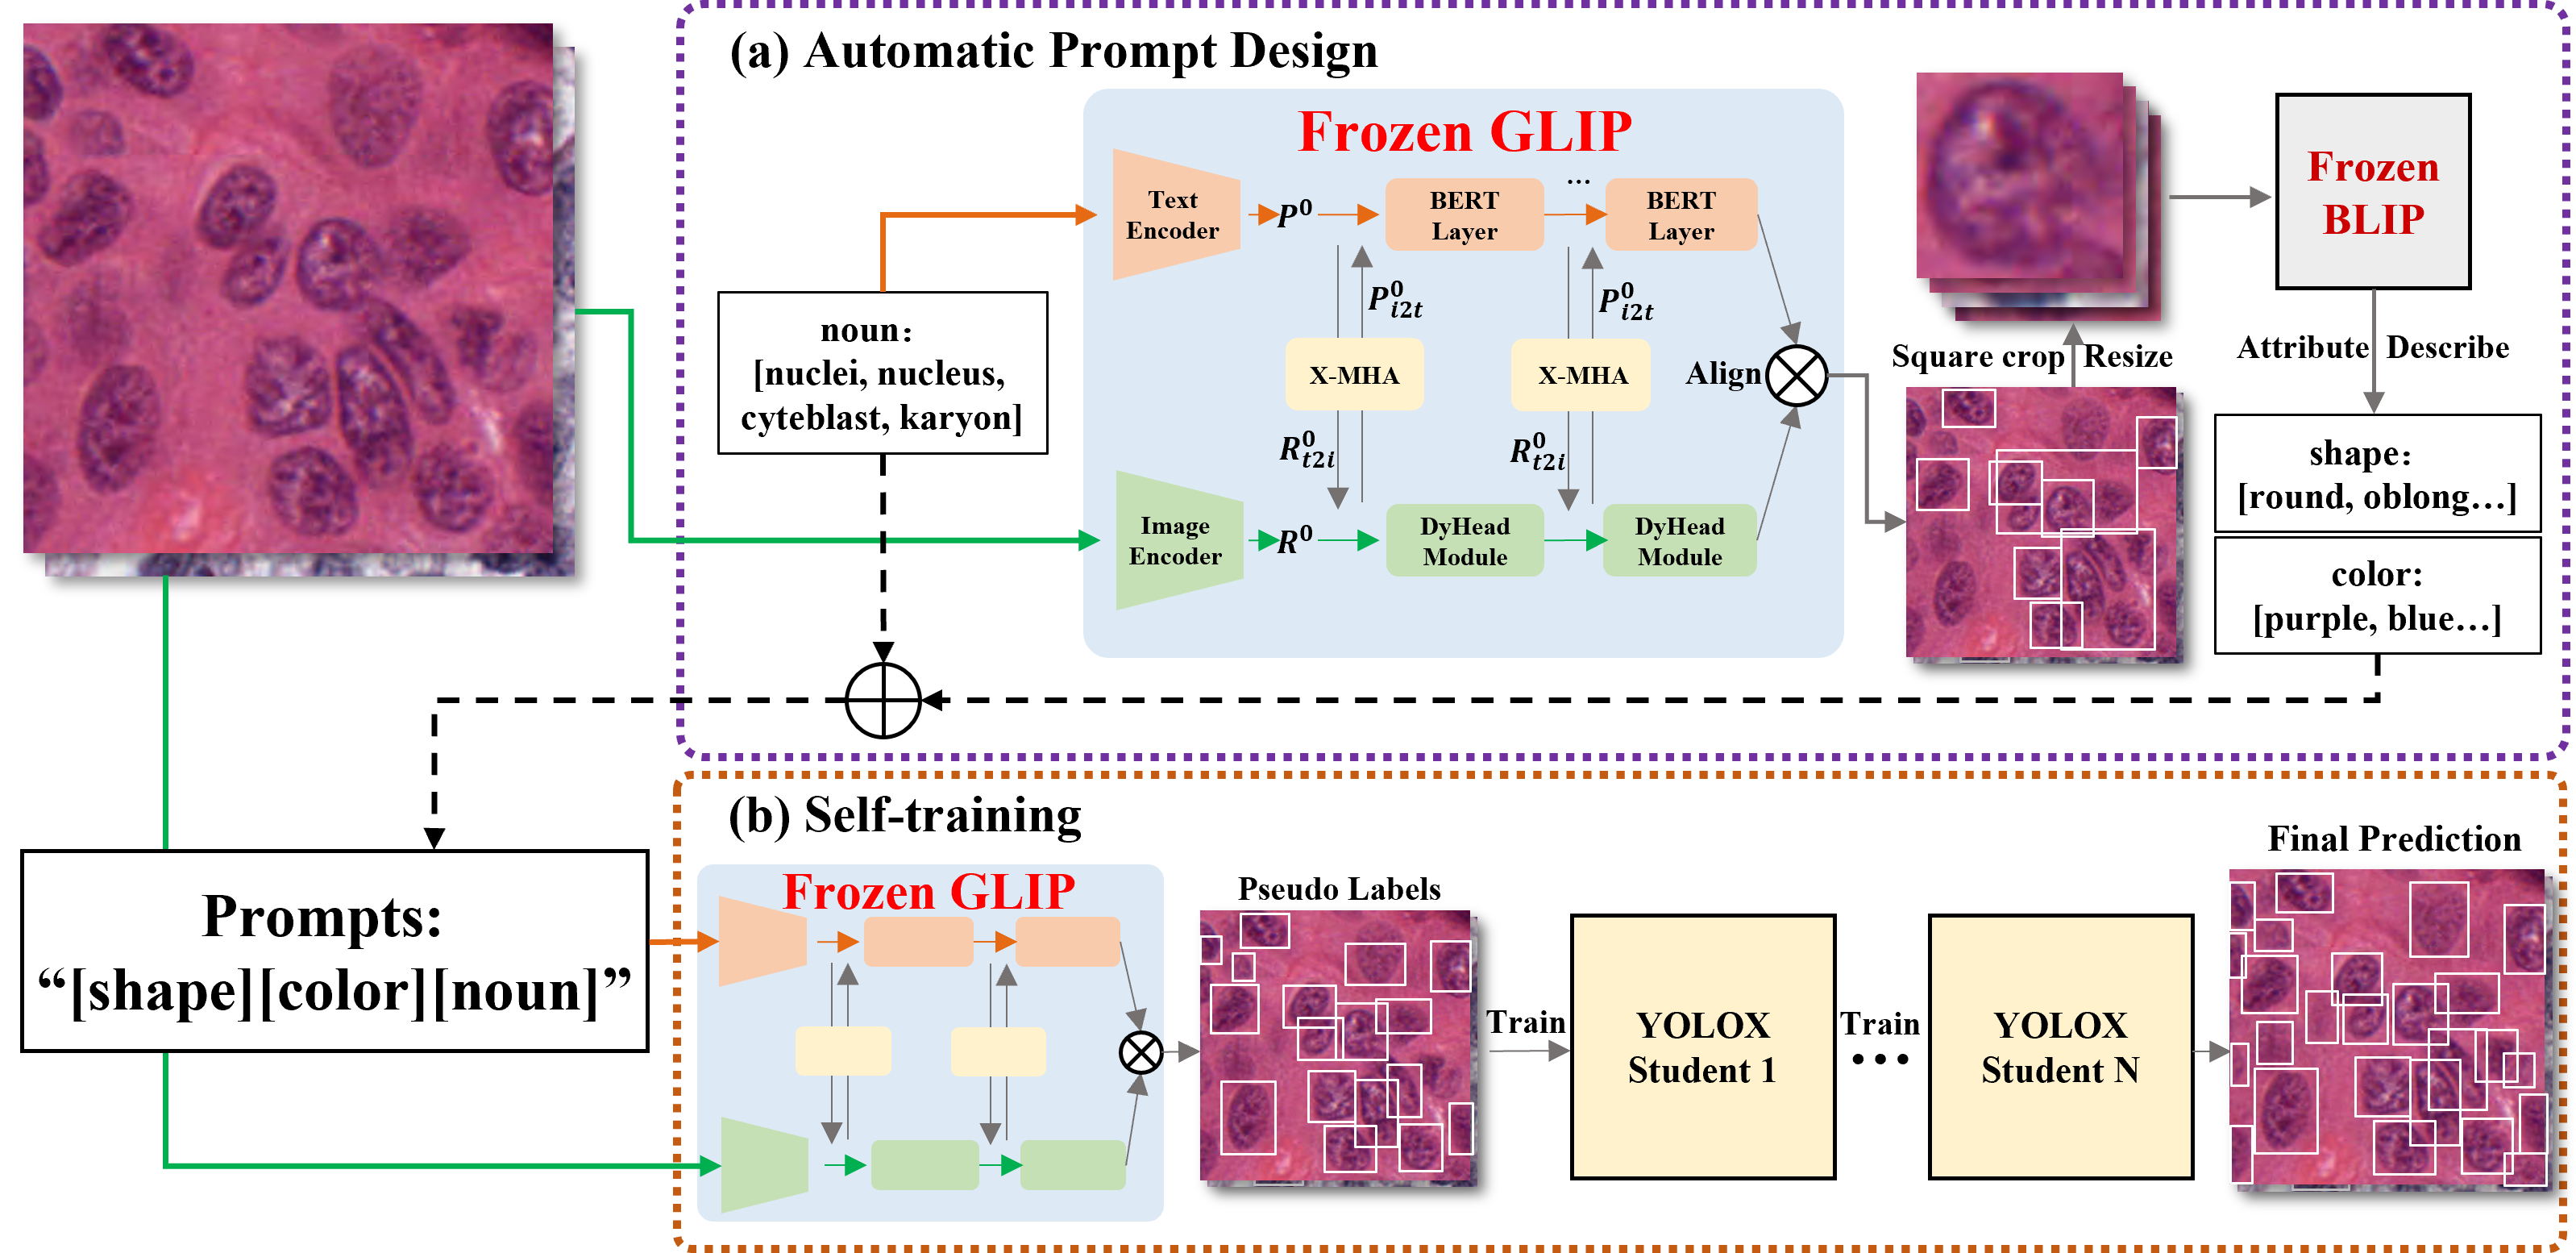
\includegraphics[width=\textwidth]{chapters/PAPERS/glip_miccai_camera_ready_version/paper2592_method.png}
  \caption{基于对象级视觉语言预训练模型 GLIP 的零样本细胞核检测框架。(a) 给定任务的目标医学名词后，基于视觉语言模型的语义属性关联特性以及图像到文本模型 BLIP，自动构造属性提示词，避免繁琐且主观的手工 prompt 工程；(b) 进一步引入自训练策略，以 GLIP 的初始预测作为伪标签，迭代训练检测器以提升召回率与定位质量。}
  \label{fig:zeroshot_framework}
\end{figure}
图 \ref{fig:zeroshot_framework} 展示了本章方法从“自动属性构造”到“零样本检测”再到“目标域自训练”的完整流程。自动属性提示的作用在于增强类名的辨识能力，使模型不再只根据粗粒度类别词汇进行定位；自训练阶段则把初始零样本预测转化为可持续优化的伪监督信号，使模型逐步吸收目标域视觉统计特征。这样的设计既延续了视觉语言模型的开放词汇能力，也兼顾了医学检测任务对稳定性的要求。

\section{实验设计}
\subsection{数据集准备}
本研究使用的数据集是MoNuSeg数据集\cite{kumar2017dataset}，它由30张大小为1000×1000的细胞核图像组成，平均每张图像有658个细胞核。继库马尔等人之后\cite{kumar2017dataset}，数据集被分成训练集和测试集，比例为16:14。 16 张训练图像作为 GLIP 的输入，生成用于自我训练的伪标签，并随机选择 4 张图像进行验证。注释仅用于测试图像的评估目的。从每个图像中提取 16 个大小为 256 × 256 的重叠图像块，并随机裁剪为 224 × 224 作为输入。在实验设置方面，使用了四个 Nvidia RTX 3090 GPU，每个 GPU 具有 24 GB 内存。在自动提示生成过程中，使用在ViT-B和CapFilt-L \cite{li2022blip}上微调的BLIP的VQA权重来生成[形状]和[颜色]属性。这些属性词通过 GPT \cite{radford2019language} 用同义词进行增强，即属性增强。目标医学名词列表首先直接设置为[“nuclei”]，并通过GPT扩充为[“nuclei”、“nucleus”、“cyteblast”、“karyon”]，即名词扩充。随后将属性词与目标医学名词组合成“[形状][颜色][名词]”格式作为 GLIP 的输入，生成边界框作为伪标签。 GLIP 使用的权重是 GLIP-L。对于自我训练细化，我们使用 YOLOX 的默认设置并遵循\cite{dopido2013semisupervised}中描述的标准自我训练方法。

\begin{table}[htbp]
  \centering
  \caption{MoNuSeg \cite{kumar2017dataset} 上的对比结果。无监督方法的最佳结果以粗体标记。}
  \label{tab:zeroshot_comparison}
  \begin{tabular}{c|c|cccc}
    \hline
    \textbf{supervision} & \textbf{method} & \textbf{mAP} & \textbf{AP50} & \textbf{AP75} & \textbf{AR} \\ \hline
    \textbf{fully-supervised} & \textbf{YOLOX (2021)} & 0.447 & 0.832 & 0.437 & 0.528 \\ \hline
    \multirow{4}{*}{\textbf{unsupervised}} & \textbf{SSNS (2020)} & 0.354 & 0.739 & 0.288 & 0.441 \\
     & \textbf{SOP (2022)} & 0.235 & 0.609 & 0.096 & 0.351 \\
     & \textbf{VLDet (2023)} & 0.173 & 0.407 & 0.112 & 0.263 \\
     & \textbf{Ours} & \textbf{0.416} & \textbf{0.808} & \textbf{0.382} & \textbf{0.502} \\ \hline
  \end{tabular}
\end{table}

\subsection{主结果与对比实验}
我们将所提出的基于 GLIP 的零样本核检测方法，与全监督检测器 YOLOX \cite{ge2021yolox} 以及代表性的无监督/零样本检测方法进行对比，包括 SSNS \cite{sahasrabudhe2020self}、SOP \cite{le2022unsupervised} 和 VLDet \cite{lin2022learning}。评估指标遵循 COCO \cite{lin2014microsoft}，报告 mAP、AP50、AP75 与 AR（召回率）。如表 \ref{tab:zeroshot_comparison} 所示，在不使用任何目标域框标注的条件下，本文方法在 mAP 与 AP50 等指标上显著优于现有无监督基线，并在整体性能上逼近全监督 YOLOX 的结果。

\begin{figure}[H]
  \centering
  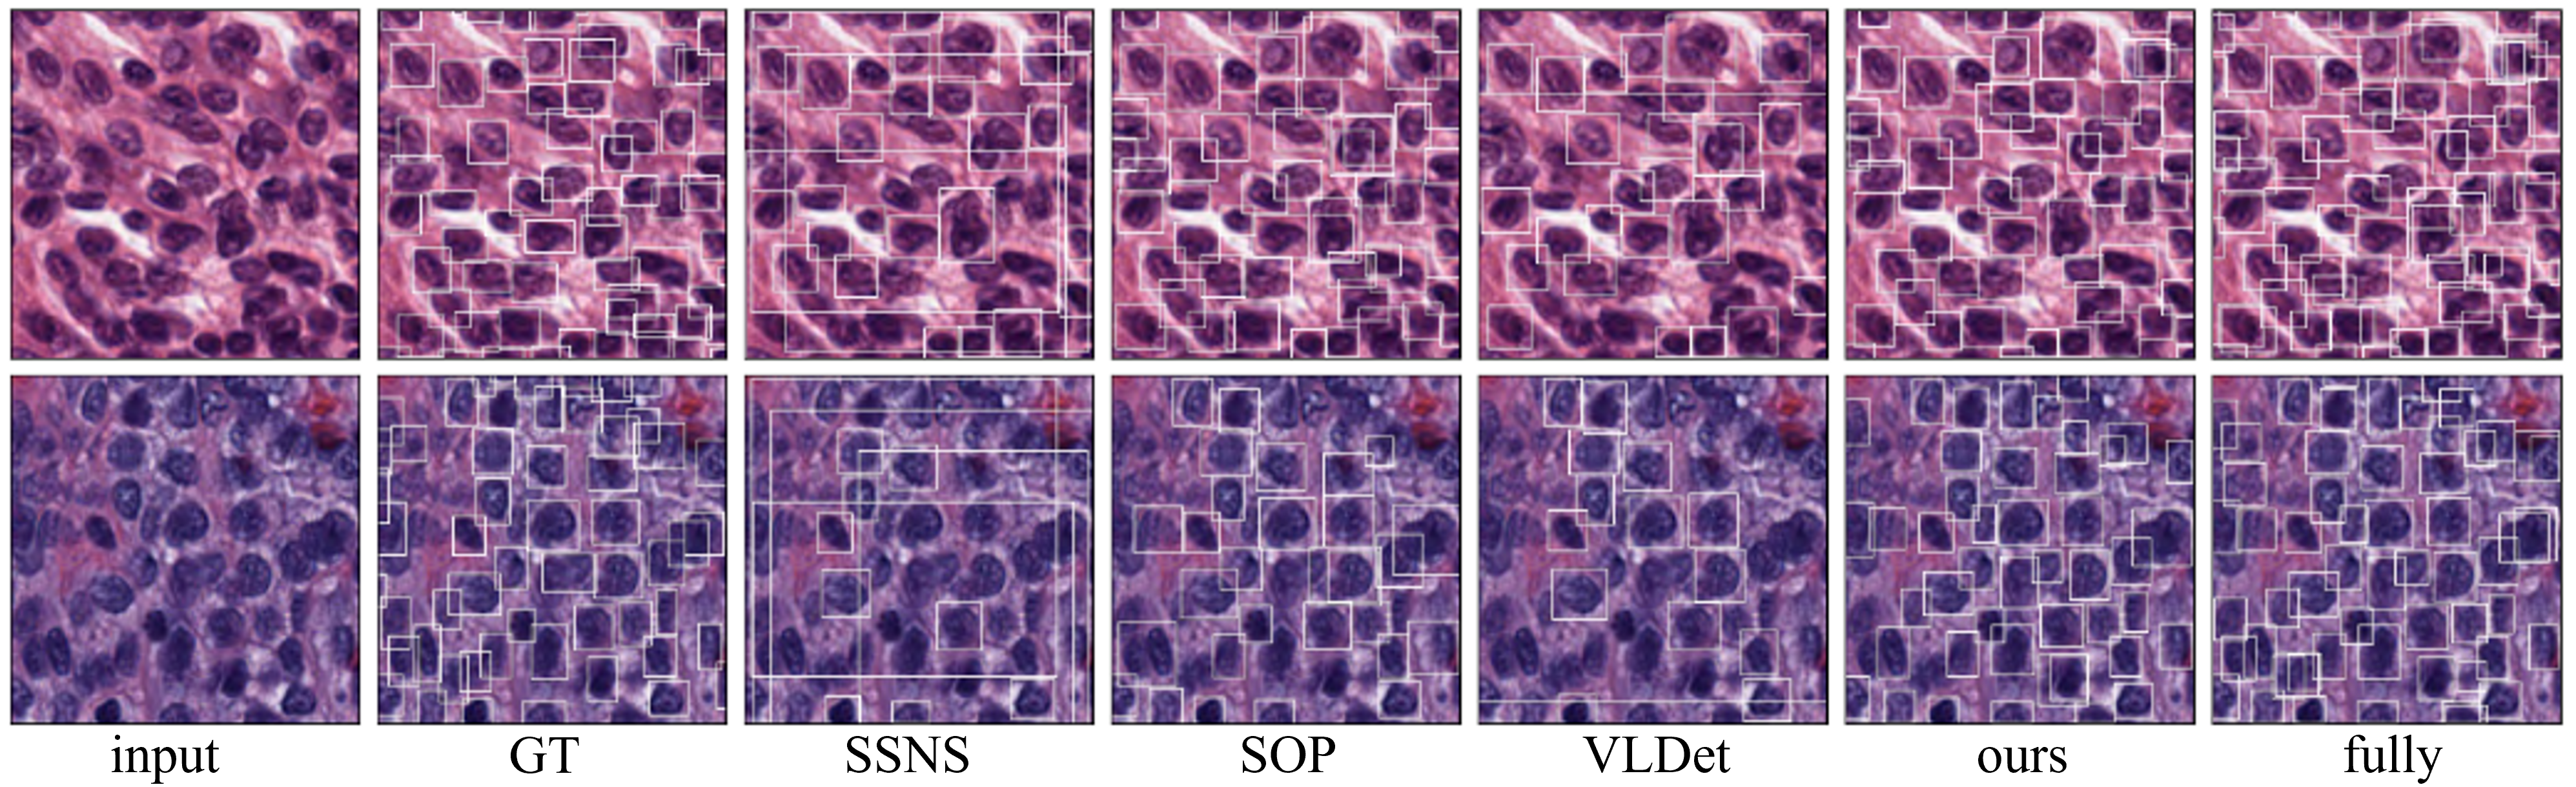
\includegraphics[width=\textwidth]{chapters/PAPERS/glip_miccai_camera_ready_version/paper2592_comparison.png}
  \caption{不同方法的检测结果可视化对比。图中白色边界框为模型预测结果，可用于观察零样本提示与自训练适配在召回率与定位质量上的差异。}
  \label{fig:zeroshot_vis}
\end{figure}

\subsection{消融实验}
\subsubsection{自动提示（prompt）构造策略}
我们首先针对 prompt 设计做消融实验，在其余设置保持一致（均使用相同的自训练流程直至收敛）的情况下对比不同提示形式，结果如表 \ref{tab:zeroshot_prompt} 所示。可以看到，仅使用医学名词串联（\textbf{noun}）时性能极差（mAP=0.064），说明医学名词与通用预训练语料之间的概念鸿沟会显著阻碍 VLPM 的直接零样本迁移。加入人工属性描述（\textbf{manual design}）后，性能大幅提升，验证了“属性描述”对核检索的重要性；但人工撰写具有经验性与主观性，难以在不同组织/染色/中心间稳定泛化。

与人工提示相比，自动提示生成能够在无模板、无人工先验的条件下生成可解释的属性词组合。进一步观察表 \ref{tab:zeroshot_prompt} 的后四行：当 prompt 从仅包含单一属性（shape 或 color）逐步扩展为同时包含形状与颜色，再结合名词形成三联体 \textbf{[shape][color][noun]} 时，检测性能呈现持续上升趋势。尤其值得注意的是，\textbf{auto: [shape][color]} 在不显式包含名词的情况下也能取得较强结果，说明 BLIP 自动生成的属性词本身已能有效刻画“核”这一目标的典型外观。

\begin{table}[htbp]
  \centering
  \renewcommand{\arraystretch}{1.1}
  \caption{不同 prompt 构造策略的消融结果（最后 4 行为自动生成提示）。最佳结果以粗体标记。}
  \label{tab:zeroshot_prompt}
  \begin{tabular}{l|rrrr}
    \hline
    \textbf{prompt design} & \textbf{mAP} & \textbf{AP50} & \textbf{AP75} & \textbf{AR} \\ \hline
    \textbf{noun} & 0.064 & 0.152 & 0.036 & 0.150 \\
    \textbf{manual design} & 0.414 & 0.757 & 0.422 & \textbf{0.509} \\ \hline
    \textbf{auto: [shape][noun]} & 0.336 & 0.604 & 0.350 & 0.434 \\
    \textbf{auto: [color][noun]} & 0.213 & 0.447 & 0.176 & 0.325 \\
    \textbf{auto: [shape][color]} & 0.413 & 0.726 & \textbf{0.438} & 0.498 \\
    \textbf{auto: [shape][color][noun]} & \textbf{0.416} & \textbf{0.808} & 0.382 & 0.502 \\ \hline
  \end{tabular}
\end{table}

\subsubsection{词汇增强（augmentation）策略}
我们进一步分析属性/名词增强对性能的影响，如表 \ref{tab:zeroshot_aug} 所示。其中，属性增强（A Aug.）通过同义词扩展形状与颜色属性；名词增强（N Aug.）将名词列表从 [``nuclei''] 扩展为 [``nuclei'', ``nucleus'', ``cyteblast'', ``karyon'']。实验表明：属性增强整体有效；而名词增强反而可能带来性能下降。其原因在于扩展得到的同义医学名词更偏“低频术语”，在 GLIP 的通用预训练语料中出现概率更低，导致提示词对齐质量下降。相对地，属性词多为自然语言中常见的外观描述，更符合 VLPM 的预训练分布，因此更稳定。

\begin{table}[htbp]
  \centering
  \renewcommand{\arraystretch}{1.1}
  \caption{词汇增强策略消融实验结果。其中 ``A Aug.'' 与 ``N Aug.'' 分别表示属性增强（attribute augmentation）与名词增强（noun augmentation）。}
  \label{tab:zeroshot_aug}
  \begin{tabular}{c|c|cccc}
    \hline
    \textbf{A Aug.} & \textbf{N Aug.} & \textbf{mAP} & \textbf{AP50} & \textbf{AP75} & \textbf{AR} \\ \hline
     &  & 0.372 & 0.725 & 0.337 & 0.464 \\
    \checkmark &  & \textbf{0.416} & \textbf{0.808} & \textbf{0.382} & \textbf{0.502} \\
     & \checkmark & 0.316 & 0.754 & 0.182 & 0.419 \\
    \checkmark & \checkmark & 0.332 & 0.659 & 0.296 & 0.434 \\ \hline
  \end{tabular}
\end{table}

\subsubsection{自训练过程与伪标签质量分析}
自训练阶段的核心作用是：将 GLIP 的初始高精度候选框转化为更高召回、更稳定的目标域检测器。表 \ref{tab:zeroshot_selftrain} 汇报了从原始 GLIP 教师（T0）到多轮 YOLOX 学生（S1--S5）的性能演化。可以观察到：原始 GLIP 的精度较高（Precision=0.678），但召回不足（Recall=0.310）；随着自训练迭代进行，召回与整体 mAP 持续提升并趋于收敛，最终达到本文的最佳配置（S4，对应表 \ref{tab:zeroshot_comparison} 的 Ours）。图 \ref{fig:miccai_selftrain} 给出了不同阶段的可视化对比。

\begin{table}[htbp]
  \centering
  \renewcommand{\arraystretch}{1.1}
  \caption{自训练策略有效性分析（IoU=0.5 下计算 Precision/Recall）。T 表示教师，S 表示学生。最佳结果以粗体标记。}
  \label{tab:zeroshot_selftrain}
  \begin{tabular}{c|cc|cccc}
    \hline
    \textbf{T/S} & \textbf{Precision} & \textbf{Recall} & \textbf{mAP} & \textbf{AP50} & \textbf{AP75} & \textbf{AR} \\ \hline
    \textbf{Raw GLIP T0} & 0.678 & 0.310 & 0.146 & 0.252 & 0.165 & 0.213 \\
    \textbf{YOLOX S1} & 0.733 & 0.706 & 0.293 & 0.636 & 0.224 & 0.397 \\
    \textbf{YOLOX S2} & 0.807 & 0.754 & 0.359 & 0.698 & 0.335 & 0.445 \\
    \textbf{YOLOX S3} & \textbf{0.814} & 0.815 & 0.404 & 0.755 & 0.395 & 0.497 \\
    \textbf{YOLOX S4} & 0.813 & \textbf{0.820} & \textbf{0.416} & \textbf{0.808} & 0.382 & 0.502 \\
    \textbf{YOLOX S5} & \textbf{0.814} & 0.807 & 0.414 & 0.742 & \textbf{0.436} & \textbf{0.509} \\ \hline
  \end{tabular}
\end{table}

为了验证“性能提升来自 VLPM 的语义伪标签，而非仅来自 YOLOX 或自训练技巧”，我们进一步用一种常见的无监督目标生成方法（超像素）替代 GLIP 生成伪标签，并保持相同自训练设置。结果如表 \ref{tab:zeroshot_superpixel} 所示，整体性能显著落后，说明高质量的零样本伪标签生成是方法成立的关键。

\begin{table}[htbp]
  \centering
  \renewcommand{\arraystretch}{1.1}
  \caption{用超像素方法生成伪标签并进行同样自训练的结果（对比说明 VLPM 伪标签的重要性）。}
  \label{tab:zeroshot_superpixel}
  \begin{tabular}{c|cccc}
    \hline
    \textbf{T/S} & \textbf{mAP} & \textbf{AP50} & \textbf{AP75} & \textbf{AR} \\ \hline
    \textbf{Superpixels T0} & 0.027 & 0.075 & 0.012 & 0.035 \\
    \textbf{YOLOX S1} & 0.260 & 0.612 & 0.162 & 0.373 \\
    \textbf{YOLOX S2} & 0.272 & 0.617 & 0.183 & 0.392 \\
    \textbf{YOLOX S3} & \textbf{0.284} & \textbf{0.655} & 0.169 & \textbf{0.404} \\
    \textbf{YOLOX S4} & 0.279 & 0.614 & \textbf{0.213} & 0.389 \\ \hline
  \end{tabular}
\end{table}

此外，我们也测试将自训练检测架构从 YOLOX 替换为 DETR \cite{carion2020end} 的可行性。如表 \ref{tab:zeroshot_detr} 所示，替换后性能仍保持在较高水平，说明方法的关键在于“语义驱动的伪标签生成”，而非强依赖某一特定检测器架构。

\begin{table}[htbp]
  \centering
  \renewcommand{\arraystretch}{1.1}
  \caption{将自训练检测架构从 YOLOX 替换为 DETR 的结果。}
  \label{tab:zeroshot_detr}
  \begin{tabular}{l|cccc}
    \hline
    \textbf{method} & \textbf{mAP} & \textbf{AP50} & \textbf{AP75} & \textbf{AR} \\ \hline
    \textbf{fully-supervised DETR} & 0.404 & 0.749 & 0.398 & 0.501 \\
    \textbf{Ours+DETR} & 0.388 & 0.731 & 0.376 & 0.487 \\ \hline
  \end{tabular}
\end{table}

\begin{figure}[H]
  \centering
  % 原图来自论文工程（PAPERS/glip\_miccai\_camera\_ready\_supplement）
  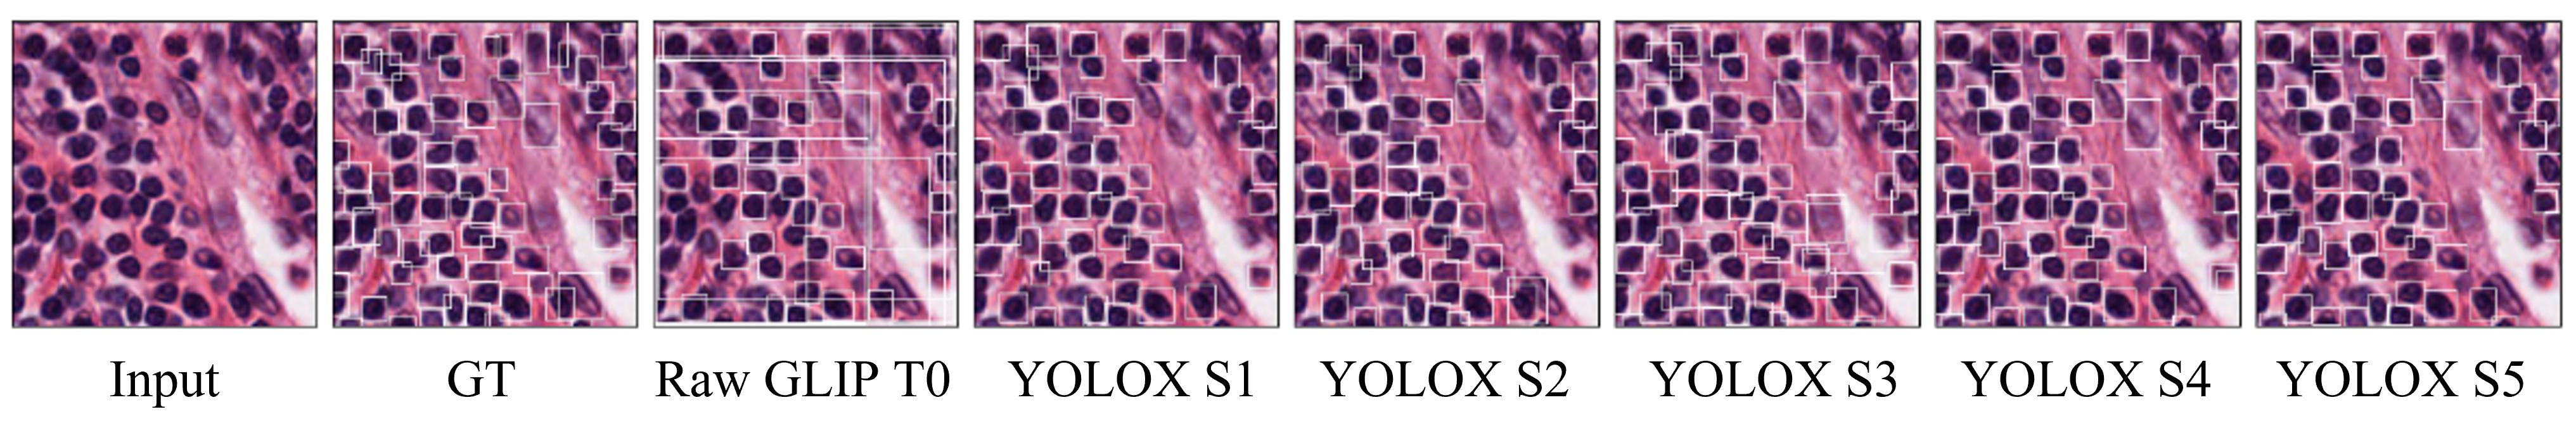
\includegraphics[width=\textwidth]{chapters/PAPERS/glip_miccai_camera_ready_supplement/self-training.png}
  \caption{MICCAI 工作中自训练策略带来的增益示意。图中展示了模型从初始零样本预测到伪标签自适配后的性能变化趋势与案例差异。}
  \label{fig:miccai_selftrain}
\end{figure}

\section{实验结果与讨论}
根据已发表工作，本章方法表明：通过自动属性提示和自训练，视觉语言预训练模型可以在没有专门检测标注的情况下，获得可用的细胞核检测能力。

\section{本章创新点总结}
本章的主要创新点体现在：第一，提出自动属性提示机制，使视觉语言模型能够在医学对象语义不足场景中获得更强提示能力；第二，将零样本视觉语言检测与自训练结合，实现从开放词汇识别到目标域适配的闭环；第三，验证了视觉语言预训练模型在医学检测中不仅可作为概念性工具，而且可作为实际有效的无标注检测入口。

\section{本章小结}
本章围绕零样本细胞核检测问题，提出自动属性提示与自训练联合框架，说明在缺少专门检测标注时，视觉语言模型依然可以通过语义构造和目标域反馈形成可用检测能力。

% 工作二：AttriPrompter / attribute-disentangled dual-modal prompting
\chapter{结合自动属性提示与自训练知识蒸馏的零样本细胞核检测}

本章在第三章基于 GLIP 的零样本细胞核检测研究基础上，进一步研究如何自动构造更适合病理图像的文本提示，以及如何利用初始零样本预测缓解密集细胞核场景下的漏检和目标重叠问题。本章方法来源于论文 \emph{AttriPrompter: Auto-Prompting with Attribute Semantics for Zero-shot Nuclei Detection via Visual-Language Pre-trained Models}，是第三章工作的扩展版本。与第三章侧重于建立零样本检测流程不同，本章重点分析提示语义粒度、提示序列顺序和知识蒸馏对检测性能的影响，并给出更系统的跨域实验。

需要特别说明的是，本章所说的“零样本”是指不使用目标测试集的人工检测标注进行训练；方法仍然可以使用目标域的无标注训练图像完成属性生成、提示筛选和伪标签自训练。因此，本章也将其称为“无标注零样本检测”或“标签免除的目标域适配”，以区分完全不接触目标域图像的严格零样本设定。

\section{研究背景与问题提出}

在数字病理分析中，细胞核检测是细胞计数、空间组织学分析、肿瘤分级和预后评估等任务的重要基础。对于 H\&E 染色病理图像，细胞核通常数量多、分布密集且相互接触。同一视野内的细胞核在颜色、形状和纹理上具有较强相似性，导致检测器容易出现漏检、误检以及相邻细胞核被合并的问题。虽然全监督检测和实例分割方法在多个数据集上取得了较好结果，但其训练依赖大量逐实例标注，而病理图像标注通常需要专业人员参与，具有成本高、耗时长和主观误差明显等特点。

为降低标注依赖，已有研究从弱监督、自监督和无监督学习等方向开展探索。弱监督方法可以使用点标注或图像级标注，但这些标注仍然需要人工制作；无监督方法则往往通过阈值、尺寸、尺度或域适配假设构造训练信号，方法性能容易受到经验性规则的影响。对于密集细胞核检测而言，如何在不使用检测标注的情况下获得可靠的初始定位，仍然是一个具有挑战性的问题。

视觉语言预训练模型（Visual-Language Pre-trained Models，VLPMs）从大规模图文对中学习视觉和文本之间的对应关系，在开放词汇识别和零样本目标检测中表现出较强的迁移能力。Grounded Language-Image Pre-training（GLIP）进一步利用短语定位数据和目标级跨模态交互，获得了比一般图像级视觉语言模型更强的目标级表示能力。然而，GLIP 的预训练数据主要来自互联网自然图像，医学图像中的细胞核概念、染色特征和密集排列模式在其语义空间中覆盖不足。直接把 ``nuclei'' 作为文本提示，往往不能稳定地激活与细胞核对应的目标级视觉表示。

因此，本章围绕两个问题展开研究：第一，能否从无标注病理图像中自动发现能够描述细胞核的属性，并将这些属性组织成适合 GLIP 的文本提示；第二，能否利用 GLIP 的初始预测作为伪标签，在不遗忘其通用目标级知识的前提下，训练更适合密集细胞核检测的学生网络。针对这两个问题，本章提出自动属性提示框架 AttriPrompter，并进一步提出自训练知识蒸馏（Self-trained Knowledge Distillation，SKD）框架。

本章的主要工作包括：
\begin{itemize}
  \item 通过提示实证分析揭示语义描述粒度和提示序列顺序对 GLIP 零样本检测的影响，说明程度属性和相关性排序对细胞核定位的重要作用。
  \item 提出 AttriPrompter 自动提示框架，利用 GLIP 和 BLIP 从无标注图像中生成形状、颜色属性，并通过同义增强、程度增强和相关性排序形成最终提示序列。
  \item 提出 SKD 框架，以 GLIP 作为教师网络，以 AttriPrompter 产生的预测作为初始伪标签，通过检测损失和特征蒸馏损失训练学生网络，并采用多轮自训练不断更新伪标签。
  \item 在 MoNuSeg 和 CoNSeP 数据集上开展对比、消融、伪标签质量、学生网络结构和跨域实验，分析各组成部分的作用及方法的适用边界。
\end{itemize}

\section{视觉语言预训练与 GLIP 基础}

视觉语言预训练模型通常从大规模图文对 $\{(x_i,t_i)\}_{i=1}^{K}$ 中学习视觉表示和文本表示之间的对应关系。设图像编码器和文本编码器分别为 $E_{\mathcal V}$ 与 $E_{\mathcal T}$，一种典型的图文对比学习目标可以写为：
\begin{equation}
\label{eq:attrip_contrastive}
\mathcal{L}_{c}=-\sum_{i=1}^{K}\log
\frac{\exp\left(s(E_{\mathcal V}(x_i),E_{\mathcal T}(t_i))\right)}
{\sum_{j=1}^{K}\exp\left(s(E_{\mathcal V}(x_i),E_{\mathcal T}(t_j))\right)},
\end{equation}
其中，$K$ 为一个批次中的图文样本数，$s(\cdot,\cdot)$ 表示经过尺度处理的余弦相似度。通过该目标，视觉编码和文本编码可以在共享语义空间中对齐，使模型能够利用文本描述识别图像内容。

与 CLIP 等主要产生图像级表示的模型相比，GLIP 直接使用短语定位图文对进行预训练。GLIP 将文本中的对象词与图像中的区域表示进行匹配，并在多个层级使用跨模态注意力实现视觉信息和语言信息的深度交互。其图像编码器能够产生与候选目标区域对应的视觉特征，文本编码器则为对象词和属性描述提供语义表示。因此，GLIP 可以通过输入文本提示完成开放词汇目标检测，这为在没有目标类别检测标注的病理图像上进行细胞核定位提供了基础。

不过，GLIP 的目标级知识主要由自然图像和网络文本构成。细胞核在自然图像中不是一个高频、边界稳定的目标类别，单独使用医学名词可能无法与预训练语料中的有效语义模式充分对应。基于这一观察，本章不直接修改 GLIP 的预训练参数，而是从输入端构造能够连接视觉外观与语言语义的属性提示。

\section{细胞核提示设计的实证分析}

\subsection{语义描述粒度的影响}

第三章已经介绍了通过属性描述增强零样本检测的基本思路。本章进一步对描述粒度进行分析。在 MoNuSeg 测试集上，分别使用仅包含类别名、加入基本形状和颜色、以及进一步加入程度描述的文本提示。结果如表~\ref{tab:attrip_PAdegree} 所示。

\begin{table}[t]
\caption{MoNuSeg 测试集上不同文本提示的 mAP。提示从上到下逐步增加语义描述的细节。}
\label{tab:attrip_PAdegree}
\begin{center}
\begin{small}
\resizebox{0.75\columnwidth}{!}{
\begin{tabular}{cc}
\toprule[1.5pt]
\textbf{文本提示} & \textbf{mAP} \\ \midrule[1.2pt]
``Nuclei.'' & 0.034 \\
``Round purple nuclei.'' & 0.046 \\
``Relatively round dark purple nuclei.'' & 0.115 \\ \bottomrule[1.5pt]
\end{tabular}
}
\end{small}
\end{center}
\vskip -0.1in
\end{table}

仅使用 ``Nuclei.'' 时，GLIP 的预测较为粗糙，并且容易在背景区域产生响应。加入 ``round'' 和 ``purple'' 后，检测性能有所提升，说明形状和颜色属性可以帮助模型缩小目标语义范围。进一步加入 ``relatively'' 和 ``dark'' 等程度描述后，mAP 从 0.046 提升到 0.115，表明描述属性的程度和细粒度同样重要。这里的程度描述不只是增加文本长度，而是为属性提供了方向和强度，例如颜色的深浅、形状的圆整程度等，使候选描述能够覆盖不同外观的细胞核。

\subsection{提示序列顺序的影响}

GLIP 通常将多个对象词或短语组织在同一个文本序列中。实验发现，当多个候选提示同时输入时，提示在序列中的位置会影响模型输出。图~\ref{fig:attrip_parelevance} 展示了按照图文相关性排序的提示序列及其预测效果。相关性较高的提示放在前部时，GLIP 的预测精度更高。

\begin{figure}[t]
\centering
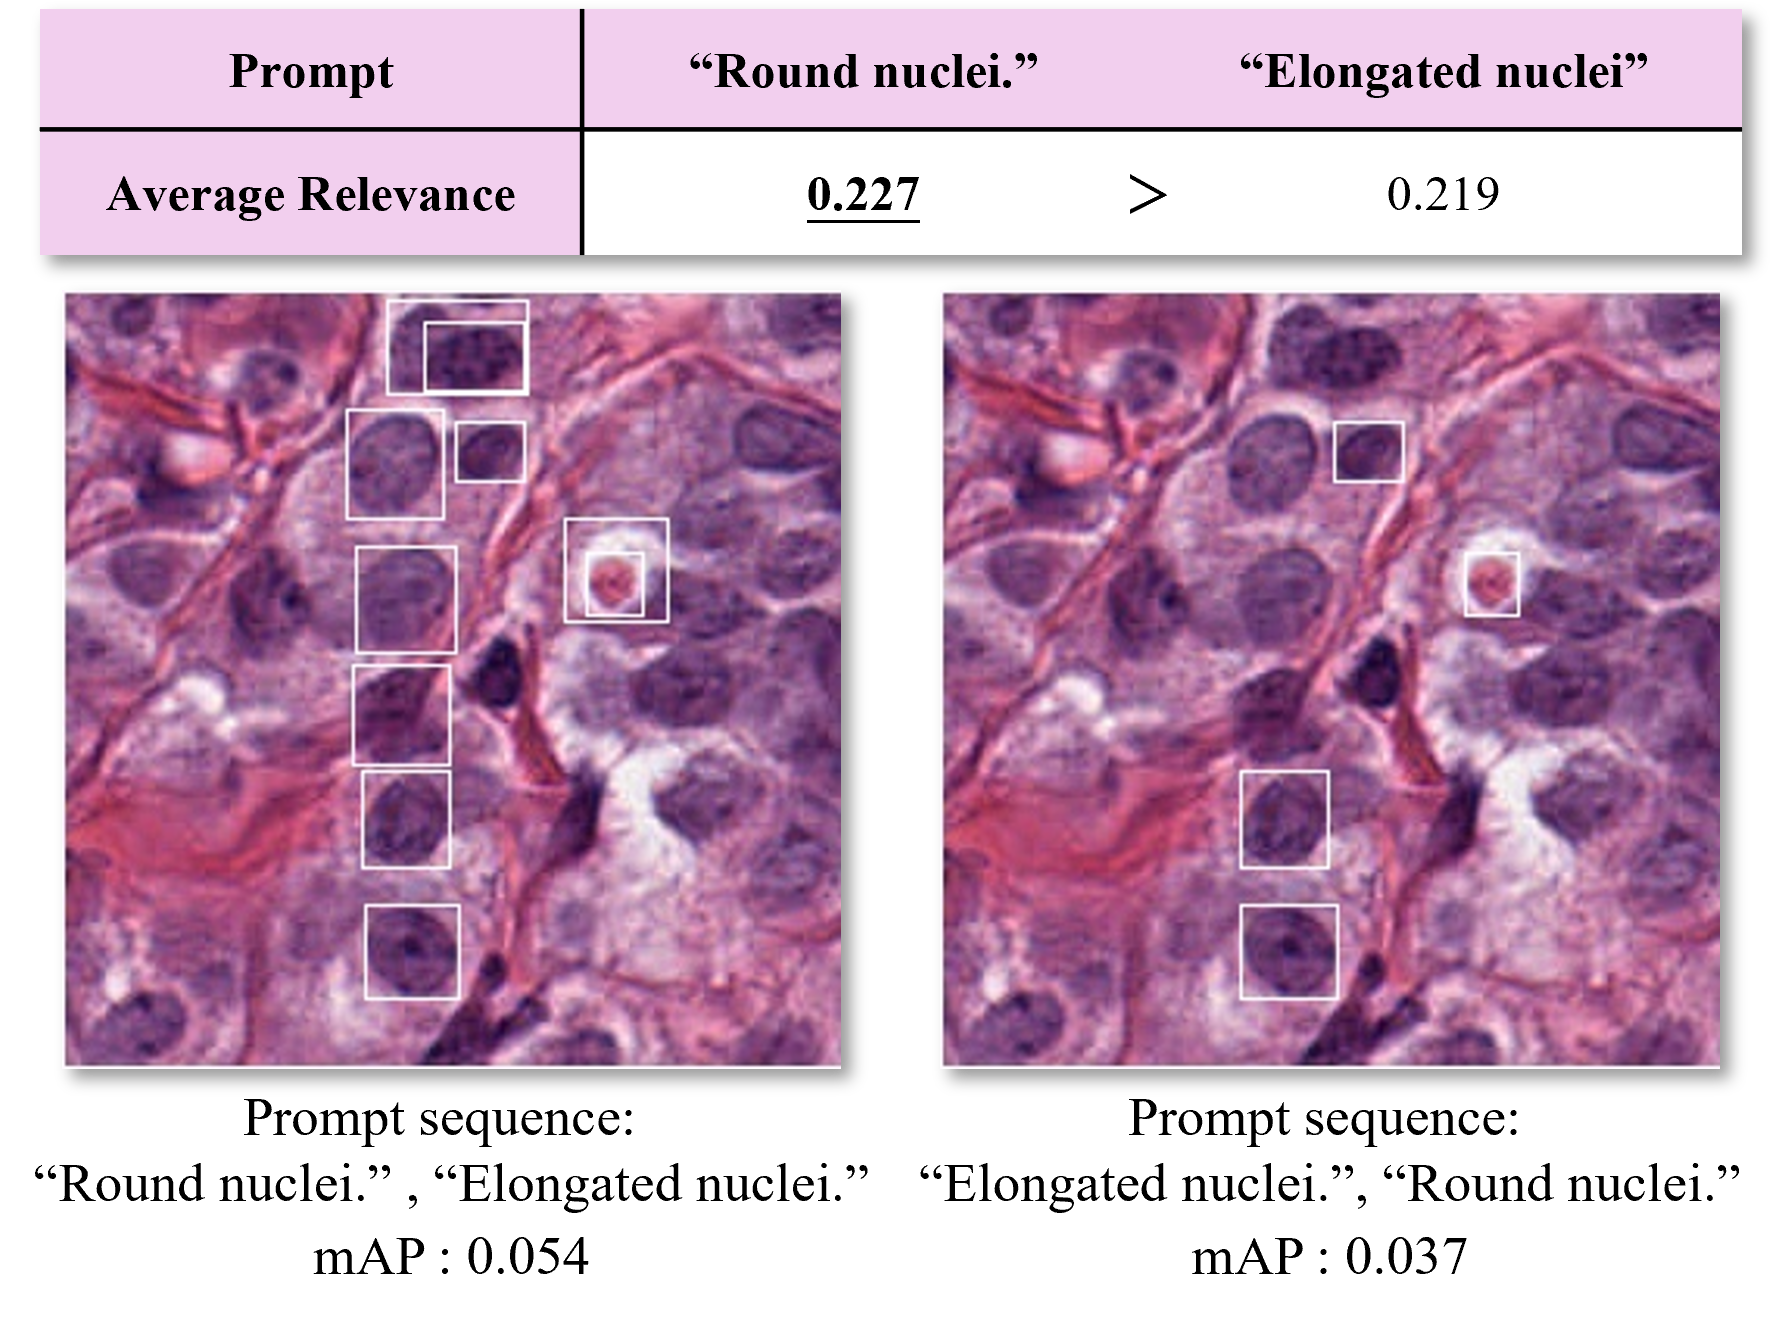
\includegraphics[width=0.95\linewidth]{chapters/PAPERS/nucleiprompter__TMI_final_version/xu2.png}
\caption{提示序列中较高相关性的提示放在前部可以提升 GLIP 的预测精度。mAP 在 MoNuSeg 测试集上统计。}
\label{fig:attrip_parelevance}
\end{figure}

这一现象说明提示序列并不是候选短语的简单集合。由于跨模态融合过程会受到序列上下文的影响，越符合当前图像域的提示越适合被放在前面。由此，本章将提示构造拆分为属性生成、属性增强和相关性排序三个步骤，以降低人工设计提示的主观性，并使提示序列能够随数据域变化而自动调整。

\section{AttriPrompter 自动属性提示框架}

AttriPrompter 的总体流程如图~\ref{fig:attrip_framework} 所示。首先，使用医学名词驱动 GLIP 产生粗略候选框，并利用这些候选框从无标注图像中裁剪细胞核区域；随后将裁剪区域输入 BLIP，通过视觉问答生成描述性词汇，再根据词频和属性类别筛选形状、颜色词。之后，使用语言模型对属性词进行同义增强和程度增强，将属性词与医学名词组合成候选提示；最后，依据候选提示和训练图像之间的平均图文相关性筛选并排序，得到输入 GLIP 的最终提示序列。

\begin{figure*}[t]
\centering
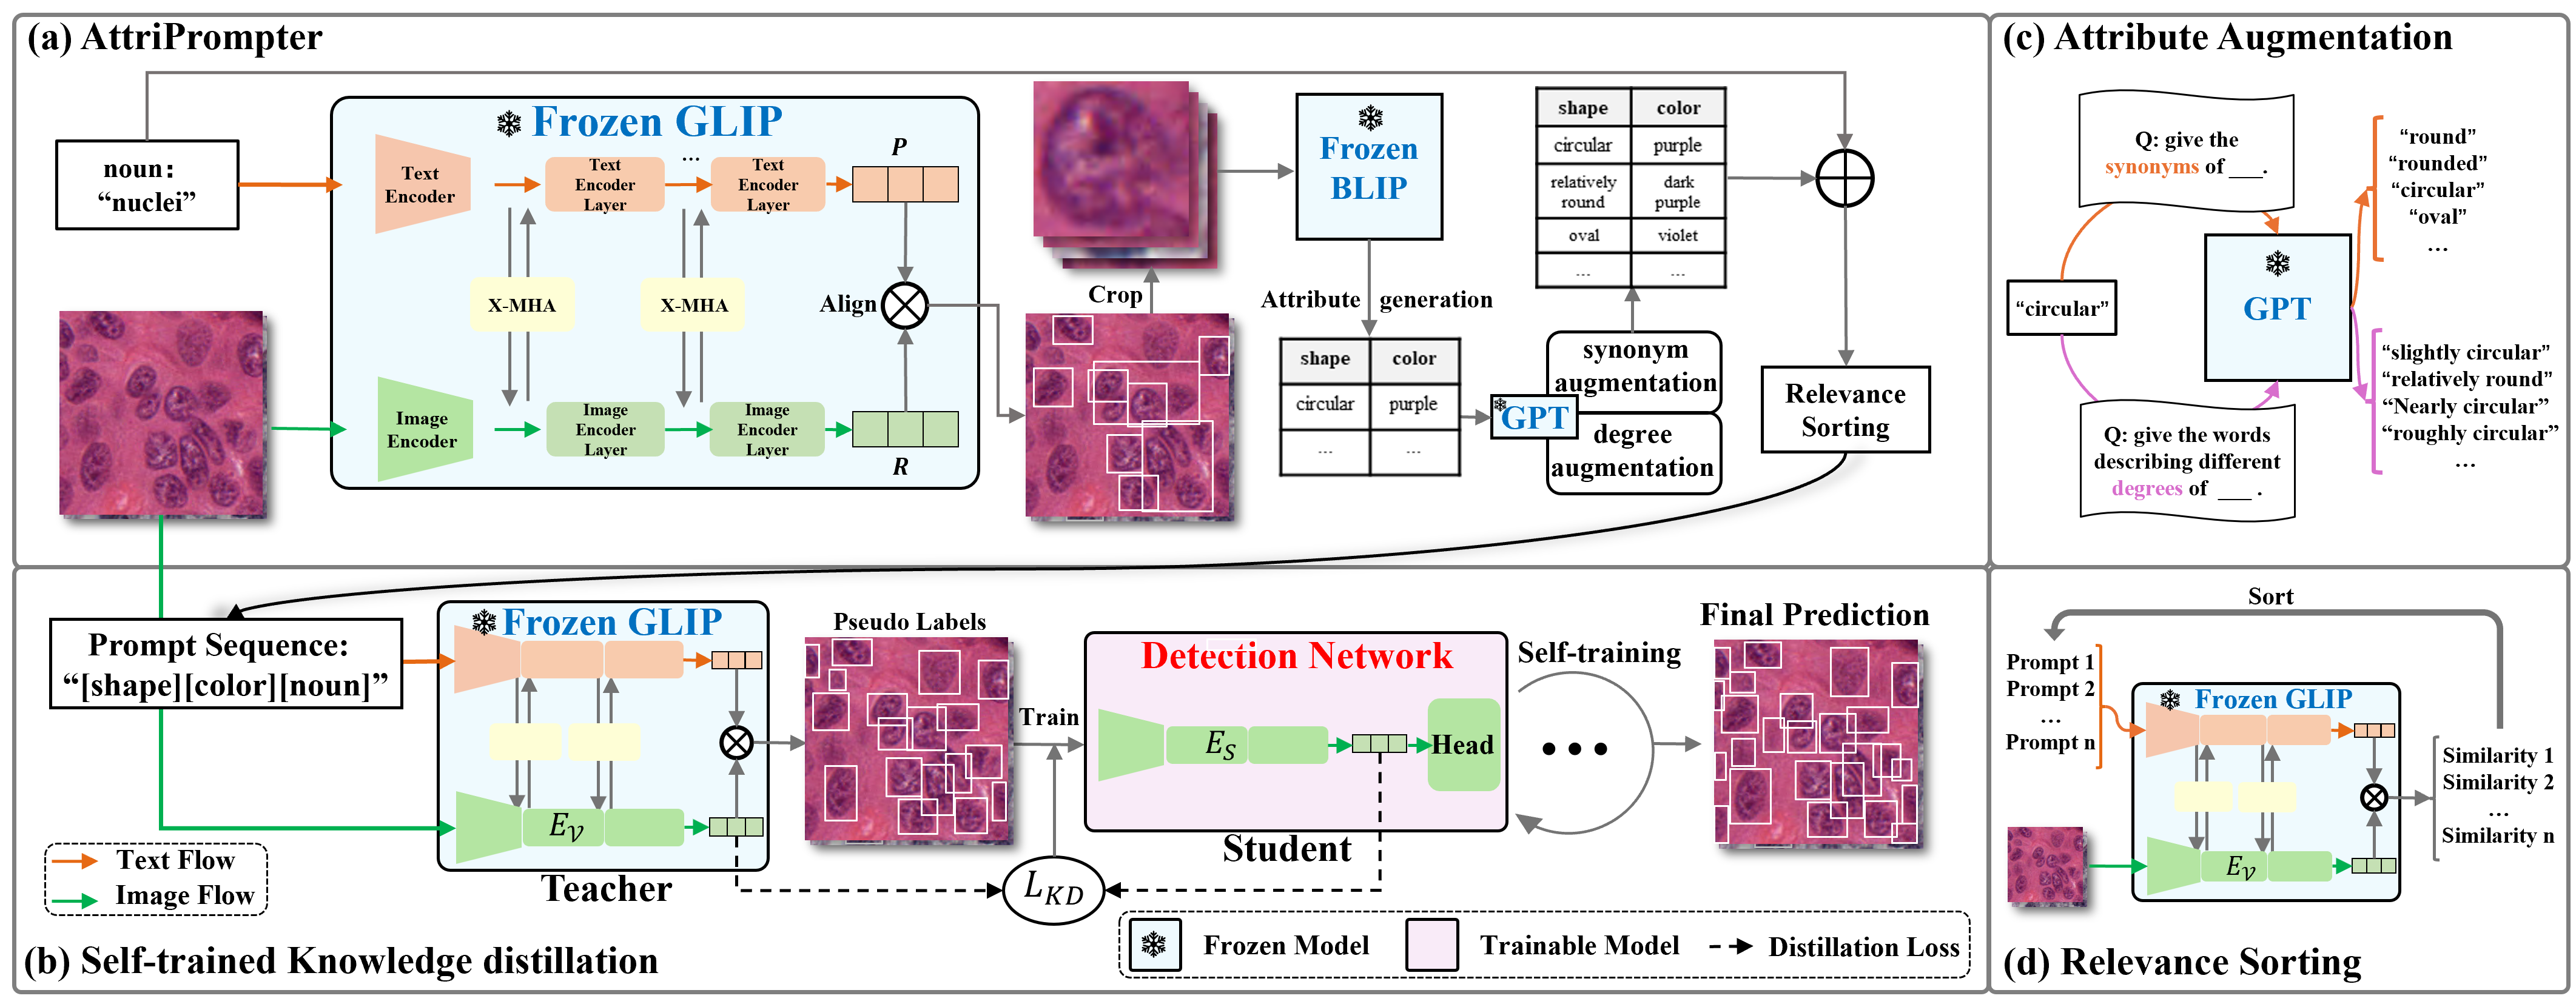
\includegraphics[width=\textwidth]{chapters/PAPERS/nucleiprompter__TMI_final_version/xu1.png}
\caption{AttriPrompter 与自训练知识蒸馏框架示意图。(a) 使用 GLIP 和 BLIP 自动生成属性，利用语言模型进行属性增强，并对候选提示进行相关性排序；(b) 基于自训练知识蒸馏进行迭代优化；(c) 属性增强过程；(d) 相关性排序过程。}
\label{fig:attrip_framework}
\end{figure*}

\subsection{属性生成}

属性生成的目标是从无标注图像中获得能够描述目标外观的词汇，避免依赖病理专家手工设计提示。具体步骤如下。

首先，将 ``nuclei'' 等医学名词作为初始提示输入 GLIP，得到细胞核的粗略候选框。此时的预测不要求具有很高的召回率，其作用是提供可供分析的候选区域。其次，将粗略候选框对应的图像区域裁剪为图像块，并输入冻结的 BLIP。BLIP 是一个兼具图像理解和文本生成能力的视觉语言模型，可以通过视觉问答回答图像块中目标的颜色和形状问题。最后，对 BLIP 生成的词汇进行词频统计和类别筛选，保留最能描述细胞核形状和颜色的属性词。

该流程具有两个优点。一方面，属性直接从目标域图像中提取，能够反映不同染色和成像条件下的细胞核外观；另一方面，属性生成依赖已经完成图文对齐的视觉语言模型，生成的词汇更有可能与 GLIP 的语义空间兼容。与完全人工设计相比，该方法减少了提示选择中的经验偏差，并保留了可解释性：每个最终提示都可以追溯到形状、颜色及其程度属性。

\subsection{属性增强}

属性生成得到的词汇数量和表达方式仍然有限。为扩大语义覆盖范围，AttriPrompter 对属性词执行同义增强和程度增强。

\textbf{同义增强。} 同义词可以在不改变基本语义的情况下提供多种语言表达。本章使用预训练语言模型对属性词进行扩展，例如将描述形状或颜色的常用词扩展为多个可能的自然语言表达。增强提示时使用的约束是：新词应当能够描述 H\&E 染色病理图像中的细胞核，而不是仅仅提供词典意义上的同义词。这样可以避免生成与目标外观无关的词汇。

\textbf{程度增强。} 仅使用 ``round'' 或 ``purple'' 等基本属性，仍然不能区分属性的强弱和程度。程度增强为每个属性添加更细粒度的描述，例如颜色的深浅、形状的圆整程度和弯曲程度。图~\ref{fig:attrip_augmentation} 中，同一框内的词表示基本语义相近的同义表达，不同框中的词表示属性程度不同。通过程度增强，候选集合覆盖了更宽的语义范围，提高了生成有效提示的概率。

\begin{figure}[t]
\centering
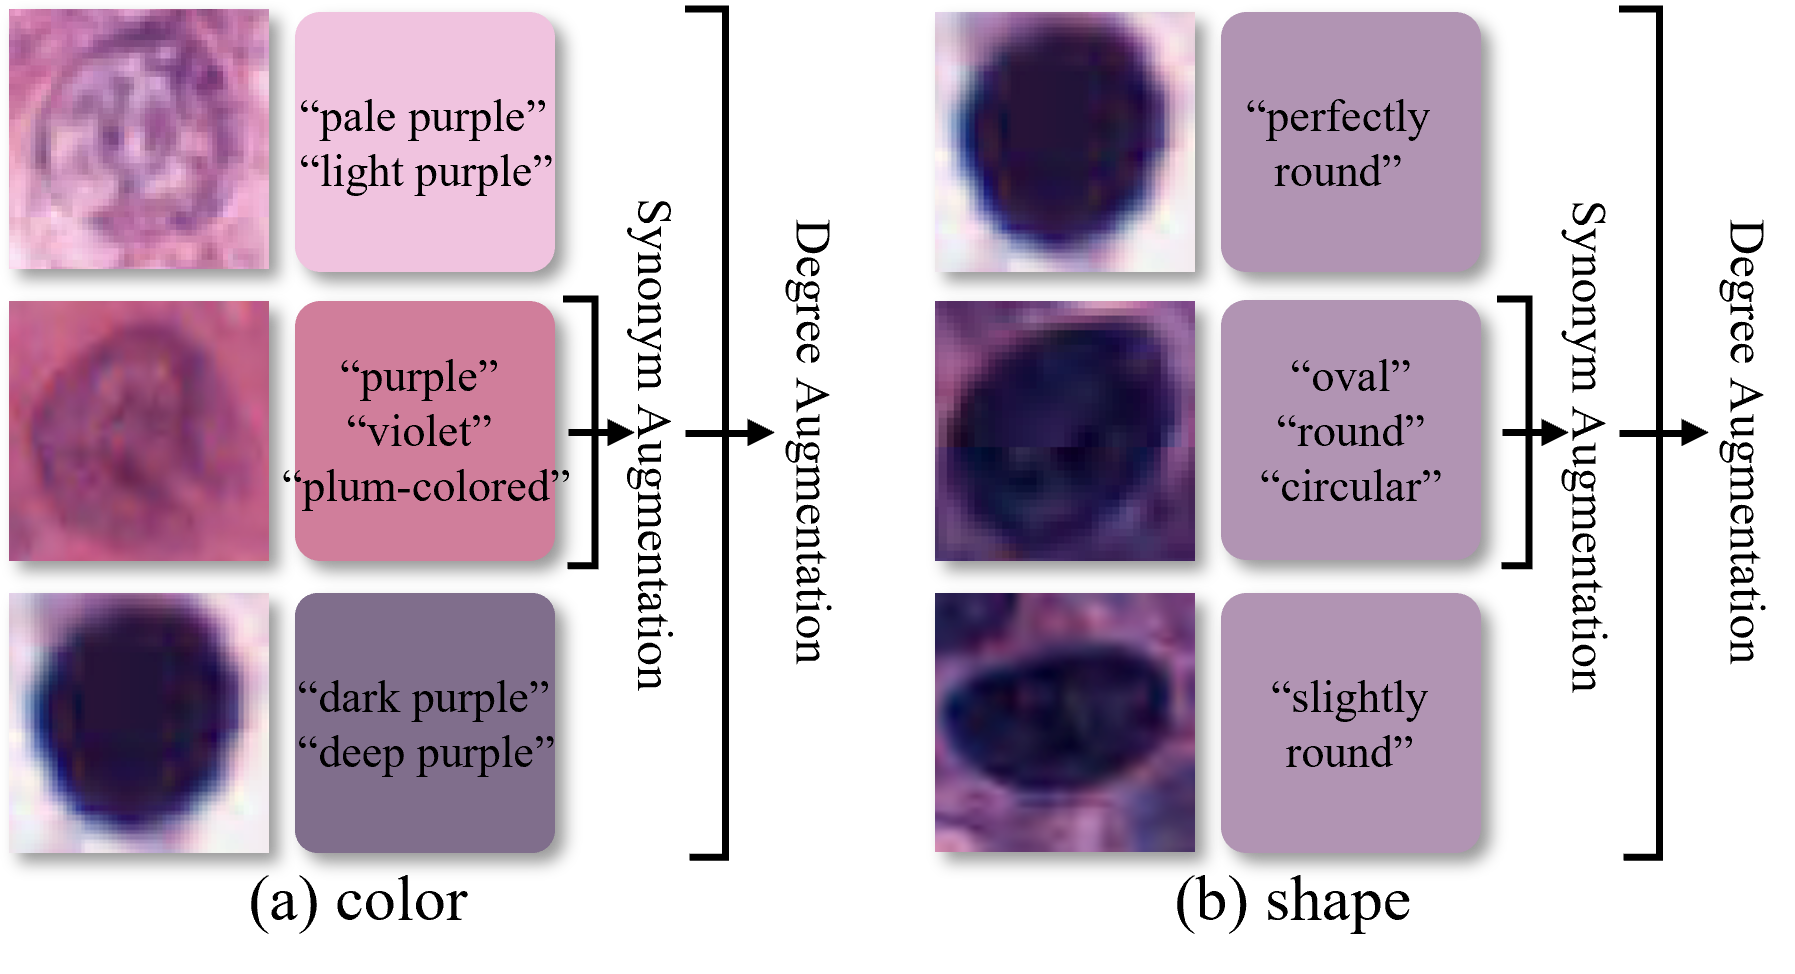
\includegraphics[width=0.95\linewidth]{chapters/PAPERS/nucleiprompter__TMI_final_version/xu3.png}
\caption{属性增强对不同细胞核外观的语义覆盖。(a) 对颜色 ``purple'' 的增强；(b) 对形状 ``round'' 的增强。同一框中的词表示同义表达，不同框中的词表示不同程度的属性描述。}
\label{fig:attrip_augmentation}
\vskip -0.15in
\end{figure}

\subsection{相关性排序}

将形状属性、颜色属性和医学名词按照模板 ``[shape] [color] [noun].'' 组合，可以形成候选检测提示。但是，程度增强也可能引入与当前图像域相关性较低的词汇。为降低无关提示带来的噪声，AttriPrompter 使用 GLIP 的视觉和文本编码结果计算提示相关性。

设训练图像 $x_i$ 中的候选区域集合为 $\mathcal{B}_i$，候选提示为 $t$。记区域 $b$ 的视觉嵌入为 $R_{i,b}=E_{\mathcal V}(x_i,b)$，提示的文本嵌入为 $P_t=E_{\mathcal T}(t)$，则候选提示在训练集上的平均相关性定义为：
\begin{equation}
\label{eq:attrip_relevance}
s(t)=\frac{1}{\sum_{i=1}^{n}|\mathcal{B}_i|}
\sum_{i=1}^{n}\sum_{b\in\mathcal{B}_i}
\frac{R_{i,b}\cdot P_t}{\|R_{i,b}\|_2\|P_t\|_2}.
\end{equation}

其中，$n$ 为用于提示生成和排序的训练图像数量。原论文为简化记号，将候选区域索引省略；式~\ref{eq:attrip_relevance} 将其显式写出，以说明相关性是对训练图像中的候选区域进行平均，而不是只计算整幅图像的单个相似度。根据 $s(t)$ 对候选提示进行降序排列，选取前 $N$ 个提示输入 GLIP。本章实验中 $N=9$，该值由 MoNuSeg 上的交叉验证确定。

相关性排序并不改变候选提示的文字内容，而是利用目标域图像确定提示的优先级。当相关性高的提示位于序列前部时，GLIP 的跨模态融合更容易先关注与当前图像外观一致的语义描述，从而改善初始预测的稳定性。

\section{自训练知识蒸馏}

\subsection{问题与总体思路}

H\&E 图像中的细胞核通常呈高密度排列，许多相邻实例之间只有很小的间隔。GLIP 虽然具有良好的目标级跨模态表示，但其预训练结构并不是专门为密集同类目标设计的，直接使用 GLIP 预测仍然容易出现漏检、误检和相邻实例重叠。若直接对目标域图像进行普通微调，又可能破坏 GLIP 原有的开放词汇知识。

为此，本章引入自训练知识蒸馏框架。GLIP 作为教师网络，通过 AttriPrompter 生成初始预测；这些预测被视为无人工标注的伪标签。随后，使用检测专用的学生网络学习伪标签，同时通过特征蒸馏损失约束学生特征与 GLIP 图像编码器特征之间的差异。学生网络的结构可以针对密集目标进行选择，实验中主要使用 YOLOX，也验证了 Mask R-CNN 的可替代性。学生网络收敛后重新生成伪标签，并开启下一轮训练，形成迭代自训练过程。

\subsection{教师网络、学生网络与训练目标}

设输入图像为 $x_i$，AttriPrompter 和 GLIP 产生的初始伪标签集合为
\begin{equation}
O_i=\{o_1,\ldots,o_{k_i}\},
\end{equation}
其中 $k_i$ 是第 $i$ 张图像中的伪标签数量。记 GLIP 的图像特征提取器为 $E_{\mathcal V}$，学生网络的特征提取器为 $E_{\mathcal S}$，学生检测头为 $\mathcal H$。知识蒸馏损失采用教师和学生特征之间的 $L_1$ 距离：
\begin{equation}
\label{eq:attrip_kd}
L_{KD}=\left\|E_{\mathcal V}(x_i)-E_{\mathcal S}(x_i)\right\|_1.
\end{equation}

学生网络的整体训练目标为：
\begin{equation}
\label{eq:attrip_student}
L_{\mathcal S}=\frac{1}{n}\sum_{i=1}^{n}
L_{Det}\left(O_i,\mathcal H(E_{\mathcal S}(x_i))\right)
+\alpha L_{KD},
\end{equation}
其中，$L_{Det}$ 表示学生检测网络的检测损失，$\alpha$ 为知识蒸馏损失权重。本章实验将 YOLOX 的特征提取器修改为与 GLIP 图像编码器相同的结构，并使用 GLIP 预训练权重进行初始化，以便进行特征对齐。需要强调的是，GLIP 在这里是教师网络，YOLOX 或 Mask R-CNN 是学生检测网络；SKD 的作用不是重新训练 GLIP，而是将其目标级知识迁移到更适合密集目标检测的网络中。

\subsection{迭代自训练}

第一轮训练结束后，使用已经收敛的学生网络重新预测训练图像，得到更新后的伪标签集合 $O_i^{(r+1)}$。随后以更新后的伪标签启动下一轮学生网络训练：
\begin{equation}
\label{eq:attrip_iterative}
L_{\mathcal S^{(r+1)}}=\frac{1}{n}\sum_{i=1}^{n}
L_{Det}\left(O_i^{(r+1)},
\mathcal H^{(r+1)}(E_{\mathcal S^{(r+1)}}(x_i))\right)
+\alpha L_{KD}.
\end{equation}

从优化角度看，这一过程可以理解为交替更新伪标签和学生网络参数：固定当前模型生成伪标签，再固定伪标签训练下一轮模型。由于后续轮次使用了学生网络对目标形态的建模能力，预测框的位置和数量可以逐步得到修正。实际实验中并非轮次越多越好，因此本章同时报告不同自训练轮次的结果，并根据验证集表现选择最终轮次。

\section{实验设置}

\subsection{数据集与数据划分}

\textbf{MoNuSeg。} MoNuSeg 包含 30 张 $1000\times1000$ 像素的细胞核图像，每张图像平均包含约 658 个细胞核。按照数据集原始划分，使用 16 张图像训练，14 张图像测试；训练过程中每个 epoch 随机选择 4 张图像用于验证。每张大图提取 16 个具有重叠区域的 $256\times256$ 图像块，并随机裁剪为 $224\times224$ 作为模型输入。训练图像仅用于自动提示生成和伪标签自训练，测试图像及其真实标注只用于最终评估。

\textbf{CoNSeP。} CoNSeP 是面向结直肠细胞核分割和表型分析的数据集，包含 41 张 $1000\times1000$ 像素的 H\&E 染色图像，这些图像来自 16 张结直肠腺癌全视野切片。除非另有说明，本章沿用与 MoNuSeg 相同的预处理方式。按照数据集默认划分，使用 26 张图像训练、1 张图像验证、14 张图像测试。

\subsection{评价指标}

本章遵循 COCO 评价协议，采用平均精度 mAP、IoU 阈值为 0.50 的 AP50、IoU 阈值为 0.75 的 AP75，以及平均召回率 AR 作为主要检测指标。mAP 综合多个 IoU 阈值下的精度，反映预测框定位精度与置信度排序的整体质量；AP50 更关注较宽松的目标匹配，AP75 对定位误差更敏感；AR 则用于衡量模型发现目标的能力。对于伪标签分析，额外使用每个伪标签与真实实例中最大 IoU 的平均值 $\mathrm{mIoU}_{\mathrm{nearest}}$，以区分“定位较准但数量不足”和“定位本身不准”两类情况。

\subsection{实现细节}

除非另有说明，实验使用 4 张具有 24 GB 显存的 NVIDIA RTX 3090 GPU。AttriPrompter 的属性生成使用在 ViT-B 和 CapFilt-L 上微调的 BLIP VQA 权重，视觉问答问题分别为 ``what is the color of the nuclei'' 和 ``what is the shape of the nuclei''。属性增强使用 ChatGPT 3.5，提示内容分别要求生成“能够描述 H\&E 染色病理图像中细胞核的同义词”和“描述某一属性不同程度的词语”。相关性排序选取 $N=9$ 个提示。主干视觉语言模型使用 GLIP-L。

在 SKD 中，将 YOLOX 的特征提取器替换为与 GLIP 图像编码器一致的结构，并使用 GLIP 预训练参数初始化；学生网络的其他训练设置采用 YOLOX 默认配置。知识蒸馏权重 $\alpha=1$，该值通过 MoNuSeg 上的四折交叉验证确定。若未特别说明，每张图像最多保留 20 个伪标签。不同的自训练轮次均使用相同的评价协议，避免把轮次变化和评价方法变化混在一起。

\section{实验结果与分析}

\subsection{与现有方法的比较}

表~\ref{tab:attrip_comparison} 汇总了本章方法与全监督、弱监督以及无监督方法的比较结果。带有 ``*'' 的方法基于医学图像，带有 ``**'' 的方法专门针对 H\&E 图像，其余方法原本面向自然图像，经过适配后用于细胞核检测。弱监督方法使用点标注作为监督信号；本章按照细胞核实例掩膜的中心生成点标注，以保持点监督定义的一致性。

\begin{table}[t]
\caption{MoNuSeg 与 CoNSeP 数据集上的检测结果（mAP、AP50、AP75 和 AR）。带 ``*'' 的方法基于医学图像，带 ``**'' 的方法专门针对 H\&E 图像。无监督方法中的最优结果以粗体表示。}
\label{tab:attrip_comparison}
\begin{center}
\resizebox{\columnwidth}{!}{
\begin{tabular}{ccccccccc}
\toprule[1.5pt]
\multirow{2}{*}{\textbf{方法}} & \multicolumn{4}{c}{\textbf{MoNuSeg}} & \multicolumn{4}{c}{\textbf{CoNSeP}} \\ \cmidrule(r){2-5} \cmidrule(r){6-9}
 & \textbf{mAP} & \textbf{AP50} & \textbf{AP75} & \textbf{AR} & \textbf{mAP} & \textbf{AP50} & \textbf{AP75} & \textbf{AR} \\ \midrule[1.2pt]
\multicolumn{9}{c}{\textbf{全监督基线}} \\
\textbf{YOLOX} & 0.447 & 0.832 & 0.437 & 0.528 & 0.388 & 0.726 & 0.384 & 0.495 \\ \hline
\multicolumn{9}{c}{\textbf{弱监督方法}} \\
\textbf{WSPointA(2019)**\cite{qu2019weakly}} & 0.341 & 0.683 & 0.272 & 0.423 & 0.301 & 0.593 & 0.277 & 0.362 \\
\textbf{WSPPointA(2020)**\cite{qu2020weakly}} & 0.367 & 0.763 & 0.302 & 0.453 & 0.308 & 0.607 & 0.281 & 0.373 \\
\textbf{WSMixedA(2020)**\cite{qu2020nuclei}} & 0.374 & 0.771 & 0.374 & 0.488 & 0.330 & 0.653 & 0.307 & 0.412 \\
\textbf{WNSeg(2022)**\cite{liu2022weakly}} & 0.404 & 0.797 & 0.416 & 0.505 & 0.364 & 0.675 & 0.329 & 0.434 \\ \hline
\multicolumn{9}{c}{\textbf{无监督方法：非视觉语言预训练模型}} \\
\textbf{SSNS(2020)**\cite{sahasrabudhe2020self}} & 0.354 & 0.739 & 0.288 & 0.441 & 0.243 & 0.458 & 0.215 & 0.294 \\
\textbf{PDAM(2020)*\cite{liu2020pdam}} & 0.275 & 0.588 & 0.228 & 0.380 & 0.166 & 0.364 & 0.132 & 0.298 \\
\textbf{DARCNN(2021)*\cite{hsu2021darcnn}} & 0.262 & 0.476 & 0.267 & 0.356 & 0.173 & 0.388 & 0.129 & 0.310 \\
\textbf{Freesolo(2022)\cite{wang2022freesolo}} & 0.292 & 0.607 & 0.248 & 0.393 & 0.222 & 0.393 & 0.246 & 0.370 \\
\textbf{SOP(2022)*\cite{le2022unsupervised}} & 0.235 & 0.609 & 0.096 & 0.351 & 0.171 & 0.387 & 0.127 & 0.304 \\
\textbf{PSM(2022)**\cite{chen2022unsupervised}} & 0.227 & 0.447 & 0.218 & 0.375 & 0.142 & 0.323 & 0.102 & 0.286 \\
\textbf{CutLER(2023)\cite{wang2023cut}} & 0.115 & 0.213 & 0.117 & 0.184 & 0.089 & 0.181 & 0.049 & 0.155 \\ \hline
\multicolumn{9}{c}{\textbf{无监督方法：视觉语言预训练模型}} \\
\textbf{VL-PLM(2022)\cite{zhao2022exploiting}} & 0.333 & 0.582 & 0.342 & 0.501 & 0.159 & 0.357 & 0.120 & 0.291 \\
\textbf{VLDet(2023)\cite{lin2022learning}} & 0.173 & 0.407 & 0.112 & 0.263 & 0.110 & 0.296 & 0.053 & 0.245 \\
\textbf{MIU-VL(2023)*\cite{qin2022medical}} & 0.070 & 0.118 & 0.076 & 0.126 & 0.066 & 0.133 & 0.045 & 0.121 \\
\textbf{VLPM-NuD(2023)**\cite{wu2023zeroshot}} & 0.416 & 0.808 & 0.382 & 0.502 & 0.359 & 0.668 & 0.363 & 0.480 \\
\textbf{本章方法**} & \textbf{0.425} & \textbf{0.819} & \textbf{0.401} & \textbf{0.511} & \textbf{0.367} & \textbf{0.669} & \textbf{0.376} & \textbf{0.488} \\ \bottomrule[1.5pt]
\end{tabular}
}
\end{center}
\end{table}

本章方法在两个数据集上均取得了无监督方法中的最佳综合结果，并接近全监督 YOLOX。非视觉语言方法通常需要依赖尺寸、阈值或域适配假设，在密集同类目标上难以同时保持精度和召回率。VL-PLM 和 VLDet 具有开放词汇能力，但没有针对 H\&E 图像进行提示和密集目标适配，因此表现有限。MIU-VL 同样基于 GLIP，但其自动提示更偏向于位置属性，适合稀疏目标检测，在细胞核密集分布场景中可能引入额外干扰。

AttriPrompter 的优势来自三个方面：自动属性生成使提示能够描述目标域外观；同义和程度增强扩大了细粒度语义覆盖；相关性排序降低了低相关提示对 GLIP 跨模态融合的干扰。进一步结合 SKD 后，学生检测器可以利用 GLIP 的目标级先验，并通过多轮伪标签更新适应密集细胞核结构。图~\ref{fig:attrip_comparison} 给出了不同方法的检测可视化结果。

\begin{figure*}[t]
\centering
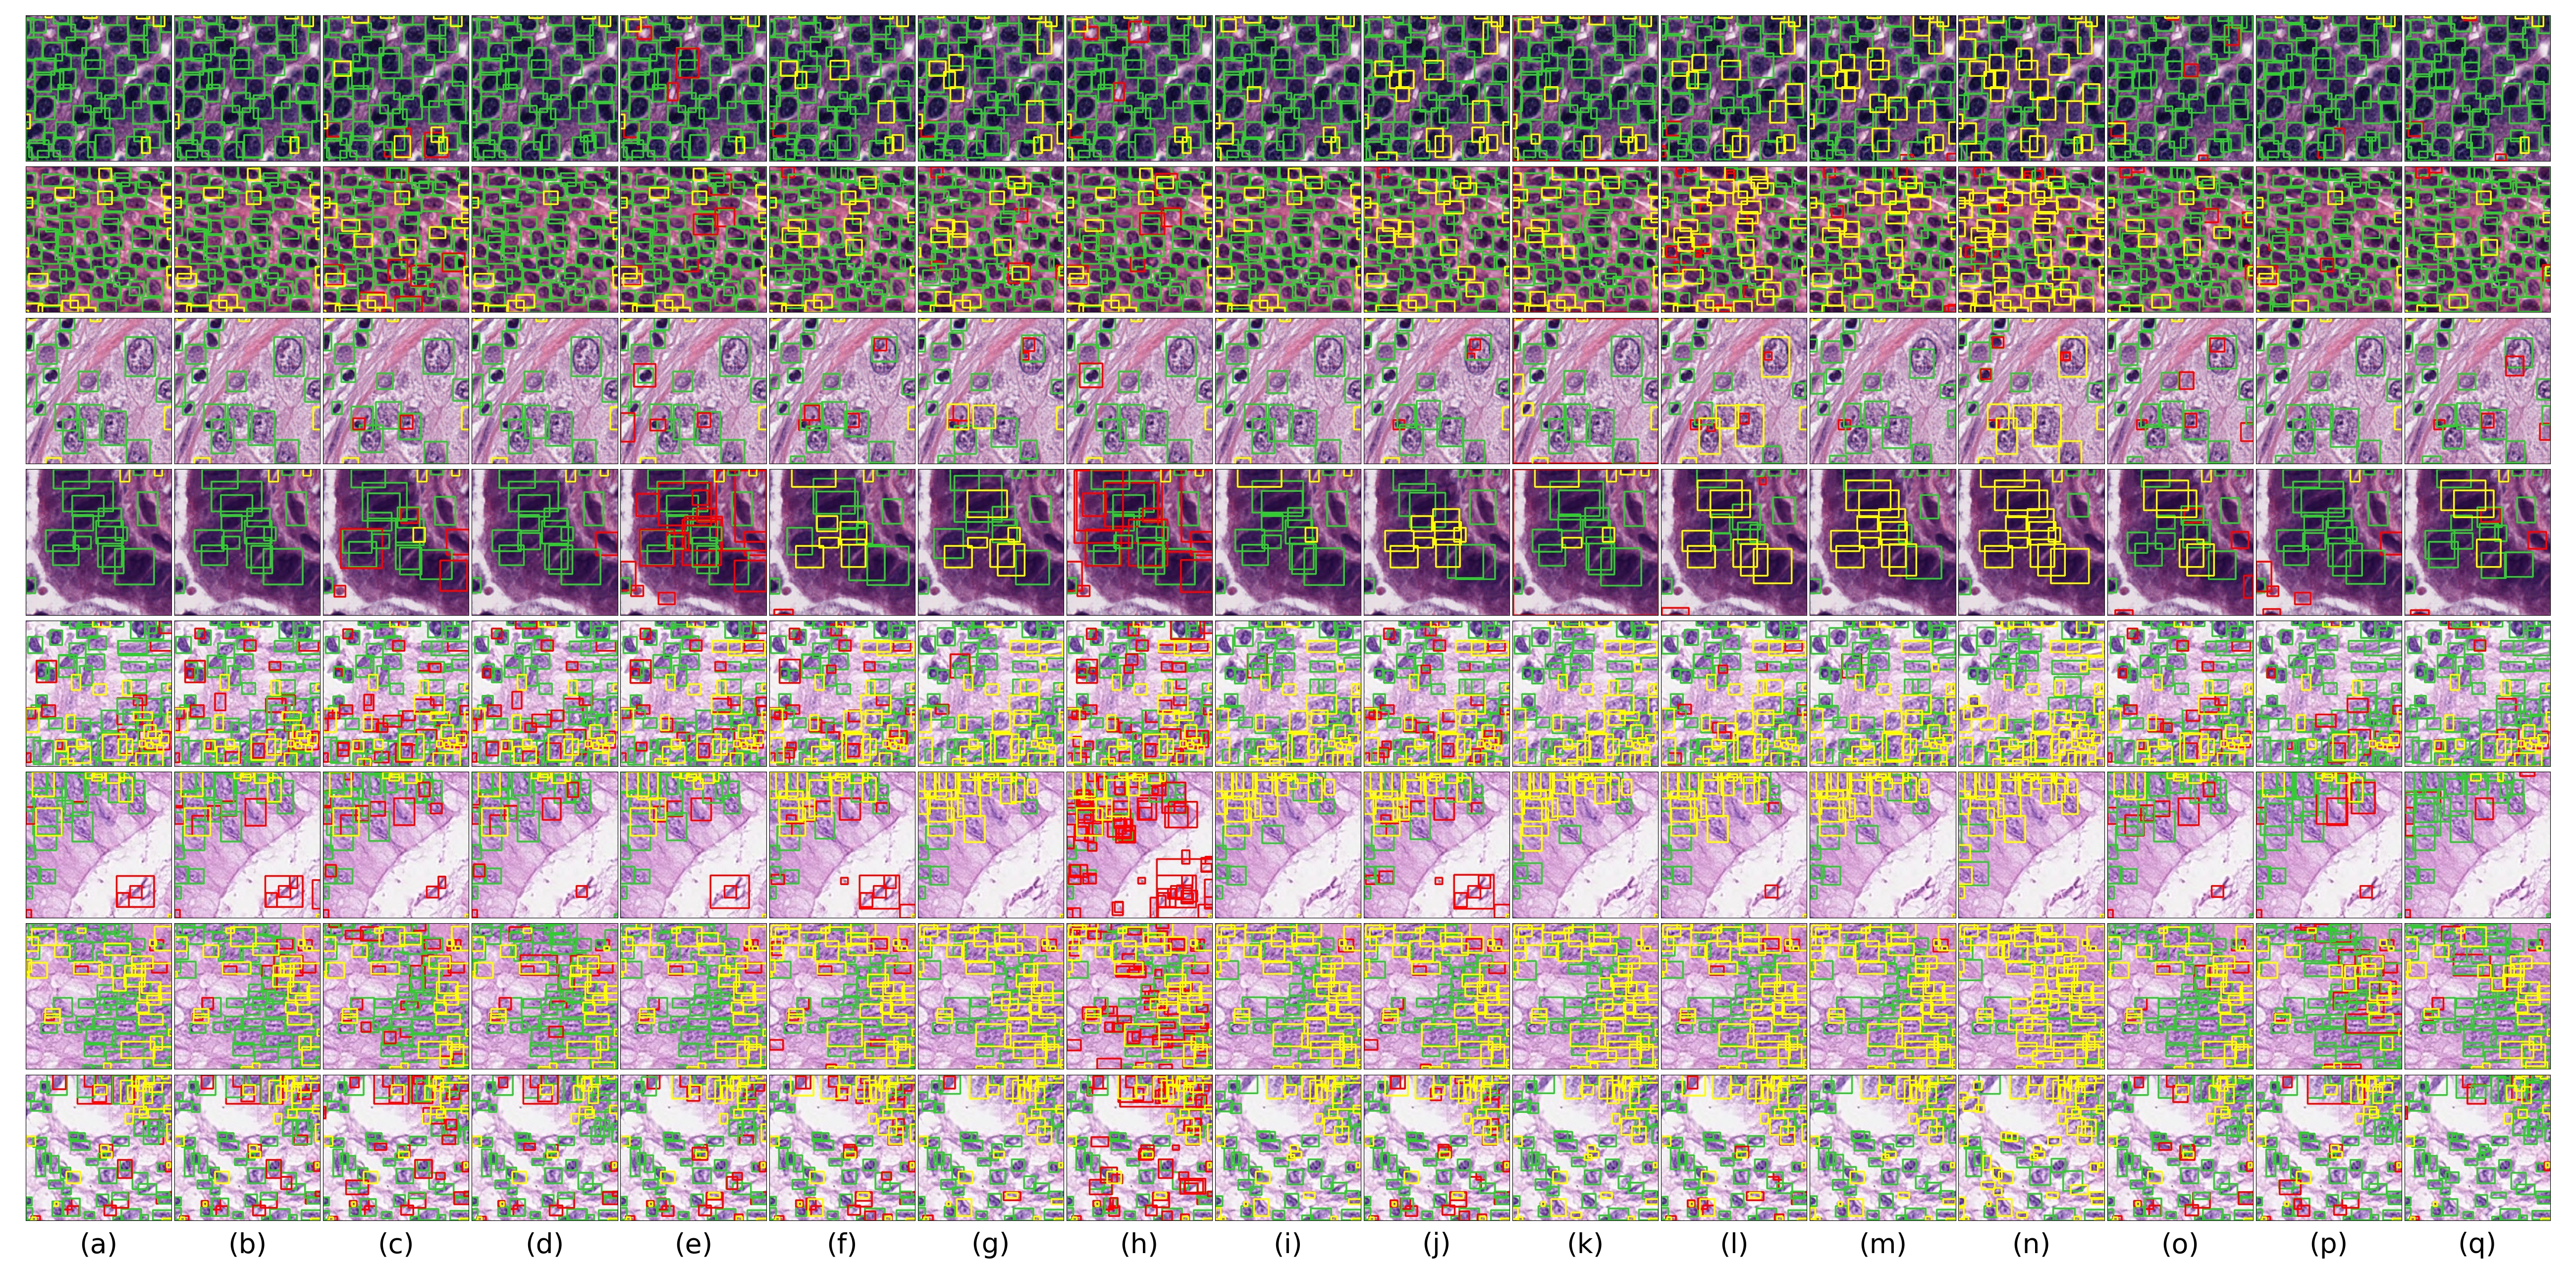
\includegraphics[width=\linewidth]{chapters/PAPERS/nucleiprompter__TMI_final_version/xu4.png}
\caption{不同方法的检测可视化结果。前四行为 MoNuSeg，后四行为 CoNSeP。绿色、红色和黄色框分别表示真阳性、假阳性和假阴性。}
\label{fig:attrip_comparison}
\end{figure*}

\subsection{自动提示与人工提示}

为直接评估提示质量，本节不引入 SKD，而是将不同提示序列直接输入 GLIP，并在相同设置下进行零样本检测。人工提示由三位病理专家分别设计，结果取平均值；其描述通常包含染色质形态、核仁以及深蓝或紫色等颜色信息。自动提示则分别使用医学名词、形状属性、颜色属性以及形状和颜色的组合。表~\ref{tab:attrip_prompt} 中的 ``Aug.'' 表示经过语言模型增强。

\begin{table}[t]
\caption{自动提示与人工提示的比较。该实验不使用 SKD，用于直接评估提示设计质量。最优结果以粗体表示。}
\label{tab:attrip_prompt}
\begin{center}
\resizebox{0.9\columnwidth}{!}{
\renewcommand{\arraystretch}{1.1}
\begin{tabular}{ccccccc}
\toprule[1.5pt]
\multicolumn{3}{c}{\multirow{2}{*}{\textbf{提示设计}}} & \multicolumn{4}{c}{\textbf{MoNuSeg}} \\ \cline{4-7}
\multicolumn{3}{c}{} & \textbf{mAP} & \textbf{AP50} & \textbf{AP75} & \textbf{AR} \\ \midrule[1.2pt]
\multicolumn{3}{c}{\textbf{人工设计}} & 0.151 & 0.259 & 0.166 & 0.210 \\ \hline
\multirow{10}{*}{\textbf{自动生成}} & \multicolumn{2}{c}{\textbf{MIU-VL(2023)\cite{qin2022medical}}} & 0.070 & 0.118 & 0.076 & 0.126 \\ \cline{2-7}
 & \textbf{属性} & \textbf{名词} & & & & \\ \cline{2-7}
 & \multirow{2}{*}{\textbf{无}} & \textbf{``Nuclei.''} & 0.034 & 0.057 & 0.038 & 0.058 \\
 & & \textbf{Aug. [noun.]} & 0.029 & 0.054 & 0.029 & 0.059 \\ \cline{2-7}
 & \textbf{[shape]} & \textbf{``Nuclei.''} & 0.097 & 0.181 & 0.097 & 0.155 \\
 & \textbf{Aug. [shape]} & \textbf{``Nuclei.''} & 0.124 & 0.255 & 0.124 & 0.191 \\ \cline{2-7}
 & \textbf{[color]} & \textbf{``Nuclei.''} & 0.009 & 0.016 & 0.010 & 0.024 \\
 & \textbf{Aug. [color]} & \textbf{``Nuclei.''} & 0.064 & 0.115 & 0.066 & 0.112 \\ \cline{2-7}
 & \textbf{[shape][color]} & \textbf{``Nuclei.''} & 0.155 & 0.285 & 0.152 & \textbf{0.239} \\
 & \textbf{Aug. [shape][color]} & \textbf{``Nuclei.''} & \textbf{0.179} & \textbf{0.310} & \textbf{0.193} & 0.220 \\ \bottomrule[1.5pt]
\end{tabular}
}
\end{center}
\end{table}

结果显示，人工提示能够取得一定性能，但依赖设计者经验，难以保证不同数据域之间的一致性。只使用类别名时性能最低；加入形状或颜色属性后性能总体提升；同时使用形状和颜色时效果最好。值得注意的是，名词同义扩展并未带来收益，可能原因是 ``cyteblast'' 和 ``karyon'' 等生僻词没有充分出现在 GLIP 的预训练语料中。相比之下，常见自然语言属性词更容易与预训练视觉语义形成对应关系。MIU-VL 的表现较低，也说明适合稀疏医学目标的位置类属性不一定适合密集细胞核检测。

\subsection{AttriPrompter 组件消融}

表~\ref{tab:attrip_promptcom} 分别去除同义增强、程度增强和相关性排序，分析三个组件的独立作用及组合效果。所有设置均不使用 SKD，以排除学生网络和自训练过程的影响。

\begin{table}[t]
\caption{AttriPrompter 组件消融实验。该实验不使用 SKD。最优结果以粗体表示。}
\label{tab:attrip_promptcom}
\begin{center}
\resizebox{0.9\columnwidth}{!}{
\begin{tabular}{ccccccc}
\toprule[1.5pt]
\textbf{同义增强} & \textbf{程度增强} & \textbf{相关性排序} & \textbf{mAP} & \textbf{AP50} & \textbf{AP75} & \textbf{AR} \\ \midrule[1.2pt]
 & & & 0.150 & 0.275 & 0.150 & 0.228 \\
\checkmark & & & 0.160 & 0.285 & 0.173 & 0.201 \\
 & \checkmark & & 0.176 & 0.304 & 0.187 & 0.213 \\
 & & \checkmark & 0.155 & 0.290 & 0.152 & \textbf{0.239} \\
\checkmark & & \checkmark & 0.174 & 0.301 & 0.188 & 0.210 \\
 & \checkmark & \checkmark & 0.178 & \textbf{0.314} & 0.187 & 0.217 \\
\checkmark & \checkmark & & 0.177 & 0.309 & \textbf{0.193} & 0.220 \\
\checkmark & \checkmark & \checkmark & \textbf{0.179} & 0.310 & \textbf{0.193} & 0.220 \\ \bottomrule[1.5pt]
\end{tabular}
}
\end{center}
\vskip -0.15in
\end{table}

三个组件组合使用时 mAP 达到 0.179，是表中最高值。程度增强和相关性排序的组合在 AP50 上达到最高值，说明细粒度属性和提示顺序分别改善了候选语义和序列上下文。仅使用同义增强的设置与第三章中较早的自动提示方案相近，性能提升相对有限。总体而言，程度增强是本章相对于基础自动属性提示的重要扩展，而相关性排序则进一步利用了 GLIP 对提示顺序的敏感性。

\subsection{不同伪标签生成方式的自训练}

为了区分“伪标签质量”和“学生网络自训练能力”的作用，本节比较 Superpixels、MIU-VL 和 AttriPrompter 三种伪标签来源。除伪标签生成方法外，三个设置均使用相同的 YOLOX 自训练框架。表~\ref{tab:attrip_selftraining} 中，Round 0 表示直接将初始伪标签与真实标注比较；Round 1 表示学生网络完成第一轮收敛后的结果；后续轮次使用前一轮学生网络生成新的伪标签。AttriPrompter 列的结果不使用知识蒸馏，以便单独考察伪标签和自训练过程。

\begin{table}[t]
\caption{采用不同伪标签生成方式进行自训练的结果。AttriPrompter（Ours）列不使用知识蒸馏。最优结果以粗体表示。}
\label{tab:attrip_selftraining}
\begin{center}
\resizebox{\columnwidth}{!}{
\begin{tabular}{ccccccccccccc}
\toprule[1.5pt]
\multirow{2}{*}{\textbf{轮次}} & \multicolumn{4}{c}{\textbf{Superpixels}} & \multicolumn{4}{c}{\textbf{MIU-VL}} & \multicolumn{4}{c}{\textbf{AttriPrompter}} \\ \cmidrule(r){2-5} \cmidrule(r){6-9} \cmidrule(r){10-13}
 & \textbf{mAP} & \textbf{AP50} & \textbf{AP75} & \textbf{AR} & \textbf{mAP} & \textbf{AP50} & \textbf{AP75} & \textbf{AR} & \textbf{mAP} & \textbf{AP50} & \textbf{AP75} & \textbf{AR} \\ \midrule[1.2pt]
\textbf{Round 0} & 0.027 & 0.075 & 0.012 & 0.035 & 0.070 & 0.118 & 0.076 & 0.126 & 0.179 & 0.310 & 0.193 & 0.220 \\
\textbf{Round 1} & 0.260 & 0.612 & 0.162 & 0.373 & 0.221 & 0.486 & 0.208 & 0.370 & 0.302 & 0.693 & 0.248 & 0.393 \\
\textbf{Round 2} & 0.272 & 0.617 & 0.183 & 0.392 & 0.242 & 0.495 & 0.239 & 0.381 & 0.358 & 0.724 & 0.326 & 0.430 \\
\textbf{Round 3} & 0.284 & 0.655 & 0.169 & 0.404 & 0.266 & 0.511 & 0.265 & 0.409 & \textbf{0.363} & 0.730 & 0.327 & 0.433 \\
\textbf{Round 4} & 0.279 & 0.614 & 0.213 & 0.389 & 0.269 & 0.515 & 0.266 & 0.416 & 0.361 & \textbf{0.732} & \textbf{0.331} & \textbf{0.435} \\ \bottomrule[1.5pt]
\end{tabular}
}
\end{center}
\vskip -0.15in
\end{table}

Superpixels 和 MIU-VL 产生的初始伪标签质量较低，虽然经过自训练后性能明显提升，但仍低于 AttriPrompter。AttriPrompter 在 Round 0 已具有较好的初始结果，经过多轮训练后 mAP 在 Round 3 达到 0.363，之后略有回落。因此，自训练过程能够改善初始伪标签，但最终性能的上限主要由初始伪标签是否具有可靠的目标语义决定。这一结果也说明本章的核心贡献并不是单纯选择更强的学生网络，而是通过属性提示充分利用 GLIP 的先验知识。

\subsection{伪标签与真实标签的质量比较}

表~\ref{tab:attrip_pseudoreal} 直接比较初始伪标签与测试集真实标注。由于密集细胞核会造成较多漏检，初始伪标签的 AR 和 AP 不高；但是，$\mathrm{mIoU}_{\mathrm{nearest}}$ 相对较高，说明已经被检测到的伪标签通常具有较好的定位精度。因此，初始伪标签的主要问题是召回率不足，而不是所有预测框都严重偏离真实细胞核。

\begin{table}[t]
\caption{初始伪标签与真实标注的直接比较。}
\label{tab:attrip_pseudoreal}
\begin{center}
\resizebox{0.86\columnwidth}{!}{
\begin{tabular}{cccccc}
\toprule[1.5pt]
\textbf{数据集} & \textbf{mAP} & \textbf{AP50} & \textbf{AP75} & \textbf{AR} & $\textbf{mIoU}_{\textbf{nearest}}$ \\ \midrule[1.2pt]
\textbf{MoNuSeg} & 0.178 & 0.312 & 0.195 & 0.217 & 0.742 \\
\textbf{CoNSeP} & 0.096 & 0.178 & 0.101 & 0.146 & 0.690 \\ \bottomrule[1.5pt]
\end{tabular}
}
\end{center}
\vskip -0.1in
\end{table}

进一步地，表~\ref{tab:attrip_semisupervised} 比较了在 SKD 框架中使用不同数量真实实例标注的结果。表中的百分比按每张训练图像的实例数量计算，例如 50\% 表示每张训练图像中一半细胞核实例使用真实框标注。AttriPrompter 伪标签的 mAP 为 0.425，高于使用 10\% 真实实例标注的结果，说明自动伪标签能够减少大量人工标注；但其整体性能仍未超过使用 50\% 真实标注的设置，表明伪标签的召回率仍有提升空间。

\begin{table}[t]
\caption{AttriPrompter 伪标签与不同比例真实标签在 SKD 框架中的比较。最优和次优结果分别以粗体和下划线表示。}
\label{tab:attrip_semisupervised}
\begin{center}
\resizebox{0.78\columnwidth}{!}{
\begin{tabular}{cccccc}
\toprule[1.5pt]
\multicolumn{2}{c}{\textbf{标签类型}} & \textbf{mAP} & \textbf{AP50} & \textbf{AP75} & \textbf{AR} \\ \midrule[1.2pt]
\multirow{4}{*}{\textbf{真实标签}} & \textbf{1\%} & 0.185 & 0.588 & 0.037 & 0.276 \\
 & \textbf{5\%} & 0.345 & 0.728 & 0.279 & 0.429 \\
 & \textbf{10\%} & 0.378 & 0.761 & 0.332 & 0.458 \\
 & \textbf{50\%} & \textbf{0.443} & \textbf{0.819} & \textbf{0.448} & \textbf{0.516} \\ \midrule
\multicolumn{2}{c}{\textbf{伪标签}} & {\ul 0.425} & \textbf{0.819} & {\ul 0.401} & {\ul 0.511} \\ \bottomrule[1.5pt]
\end{tabular}
}
\end{center}
\vskip -0.15in
\end{table}

\subsection{最优提示词分析}

相关性排序的一个优点是可以输出每个提示的相关性分数和单提示预测结果。表~\ref{tab:attrip_detailprompt} 展示 MoNuSeg 上相关性最高的 15 个候选提示，其中前 9 个提示在交叉验证后被选为最终提示，后续提示仅作为对照。结果显示，包含 ``slightly round''、``dark purple''、``moderately round'' 和 ``circular'' 的提示相对有效；这些词既符合 H\&E 染色细胞核的常见外观，也较容易与 GLIP 预训练阶段的自然语言形成对应。相反，``elliptical'' 和 ``elongated'' 等词在自然语言语料中的使用频率较低，可能导致跨模态匹配较弱。

\begin{table}[t]
\caption{MoNuSeg 上最优提示词的定量分析。前 9 个提示通过交叉验证选取，后续提示被舍弃并以灰色标记。}
\label{tab:attrip_detailprompt}
\begin{center}
\resizebox{0.98\columnwidth}{!}{
\begin{tabular}{cccc}
\toprule[1.5pt]
\textbf{排序} & \textbf{提示词} & \textbf{相关性} & \textbf{单提示 mAP} \\ \midrule[1.2pt]
1 & ``slightly round dark purple nuclei.'' & 0.317 & 0.116 \\
2 & ``slightly round purple nuclei.'' & 0.315 & 0.128 \\
3 & ``moderately round purple nuclei.'' & 0.312 & 0.104 \\
4 & ``moderately round dark purple nuclei.'' & 0.311 & 0.103 \\
5 & ``slightly round violet nuclei.'' & 0.311 & 0.099 \\
6 & ``circular purple nuclei.'' & 0.306 & 0.063 \\
7 & ``circular dark purple nuclei.'' & 0.304 & 0.067 \\
8 & ``circular violet nuclei.'' & 0.303 & 0.061 \\
9 & ``moderately round violet nuclei.'' & 0.302 & 0.057 \\
\rowcolor{lightgray} 10 & ``mostly round rich purple nuclei.'' & 0.299 & 0.054 \\
\rowcolor{lightgray} 11 & ``moderately round rich purple nuclei.'' & 0.299 & 0.051 \\
\rowcolor{lightgray} 12 & ``elliptical purple-blue nuclei.'' & 0.298 & 0.041 \\
\rowcolor{lightgray} 13 & ``elongated dark purple nuclei.'' & 0.296 & 0.040 \\
\rowcolor{lightgray} 14 & ``slightly circular plum-colored nuclei.'' & 0.294 & 0.033 \\
\rowcolor{lightgray} 15 & ``elliptical vibrant purple nuclei.'' & 0.294 & 0.032 \\
\rowcolor{lightgray} \multicolumn{4}{c}{\cellcolor{lightgray}...} \\ \bottomrule[1.5pt]
\end{tabular}
}
\end{center}
\vskip -0.15in
\end{table}

\subsection{知识蒸馏损失消融}

为了验证 $L_{KD}$ 是否能够帮助学生网络保留 GLIP 的目标级先验，表~\ref{tab:attrip_kd} 在人工提示、仅使用 ``Nuclei.'' 和完整 AttriPrompter 三种提示设置下分别去除或加入知识蒸馏损失。无论使用何种提示，加入 $L_{KD}$ 后 mAP 和 AR 均得到提升；在完整 AttriPrompter 下，mAP 从 0.412 提升到 0.425，说明知识蒸馏可以有效改善自训练结果。

\begin{table}[t]
\caption{知识蒸馏损失 $L_{KD}$ 的消融实验。不使用 $L_{KD}$ 时，学生网络仅由检测损失 $L_{Det}$ 训练。最优结果以粗体表示。}
\label{tab:attrip_kd}
\begin{center}
\resizebox{0.9\columnwidth}{!}{
\begin{tabular}{cccccc}
\toprule[1.5pt]
\textbf{提示设计} & $\boldsymbol{L_{KD}}$ & \textbf{mAP} & \textbf{AP50} & \textbf{AP75} & \textbf{AR} \\ \midrule[1.2pt]
\multirow{2}{*}{\textbf{人工提示}} & & 0.409 & 0.801 & 0.383 & 0.493 \\
 & \checkmark & 0.418 & 0.811 & 0.392 & 0.504 \\ \hline
\multirow{2}{*}{\textbf{``Nuclei.''}} & & 0.324 & 0.696 & 0.316 & 0.381 \\
 & \checkmark & 0.352 & 0.711 & 0.334 & 0.414 \\ \hline
\multirow{2}{*}{\textbf{AttriPrompter}} & & 0.412 & 0.805 & 0.385 & 0.498 \\
 & \checkmark & \textbf{0.425} & \textbf{0.819} & \textbf{0.401} & \textbf{0.511} \\ \bottomrule[1.5pt]
\end{tabular}
}
\end{center}
\end{table}

\subsection{不同学生检测网络结构}

SKD 的学生网络并不限定为 YOLOX。为验证方法的结构可迁移性，本节将学生网络替换为 Mask R-CNN，并保持伪标签生成、蒸馏损失和自训练流程不变。Mask R-CNN 训练时每张图像最多使用 100 个真实或伪标签实例，RPN 在训练和测试阶段的非极大值抑制阈值分别设置为 0.9 和 0.7，其余参数采用 COCO 默认配置。表~\ref{tab:attrip_architecture} 显示，使用 Mask R-CNN 时本章方法仍然优于相同学生结构下的 VLPM-NuD，说明性能提升主要来自提示和知识迁移机制，而不是某一种特定检测头。

\begin{table}[t]
\caption{不同学生网络结构下的实验结果。}
\label{tab:attrip_architecture}
\begin{center}
\resizebox{0.9\columnwidth}{!}{
\begin{tabular}{cccccc}
\toprule[1.5pt]
\textbf{学生网络} & \textbf{方法} & \textbf{mAP} & \textbf{AP50} & \textbf{AP75} & \textbf{AR} \\ \midrule[1.2pt]
\multirow{3}{*}{\textbf{YOLOX}} & \textbf{全监督} & 0.447 & 0.832 & 0.437 & 0.528 \\
 & \textbf{VLPM-NuD} & 0.416 & 0.808 & 0.382 & 0.502 \\
 & \textbf{本章方法} & 0.425 & 0.819 & 0.401 & 0.511 \\ \hline
\multirow{3}{*}{\textbf{Mask R-CNN}} & \textbf{全监督} & 0.385 & 0.751 & 0.358 & 0.466 \\
 & \textbf{VLPM-NuD} & 0.350 & 0.718 & 0.321 & 0.412 \\
 & \textbf{本章方法} & 0.371 & 0.734 & 0.336 & 0.446 \\ \bottomrule[1.5pt]
\end{tabular}
}
\end{center}
\vskip -0.15in
\end{table}

\section{跨域能力分析}

医学图像可能来自不同医疗中心、扫描设备或染色流程，域偏移会改变细胞核的颜色、纹理和形状分布。因此，本节开展两组跨域实验。第一组实验检验 AttriPrompter 本身的跨域能力：使用一个数据集生成提示，再在另一个数据集上进行 SKD 和测试。第二组实验检验完整系统的 domain shift 性能：在源域训练整个系统，在不同目标域测试。实验流程如图~\ref{fig:attrip_cross_domain} 所示。

\begin{figure}[t]
\centering
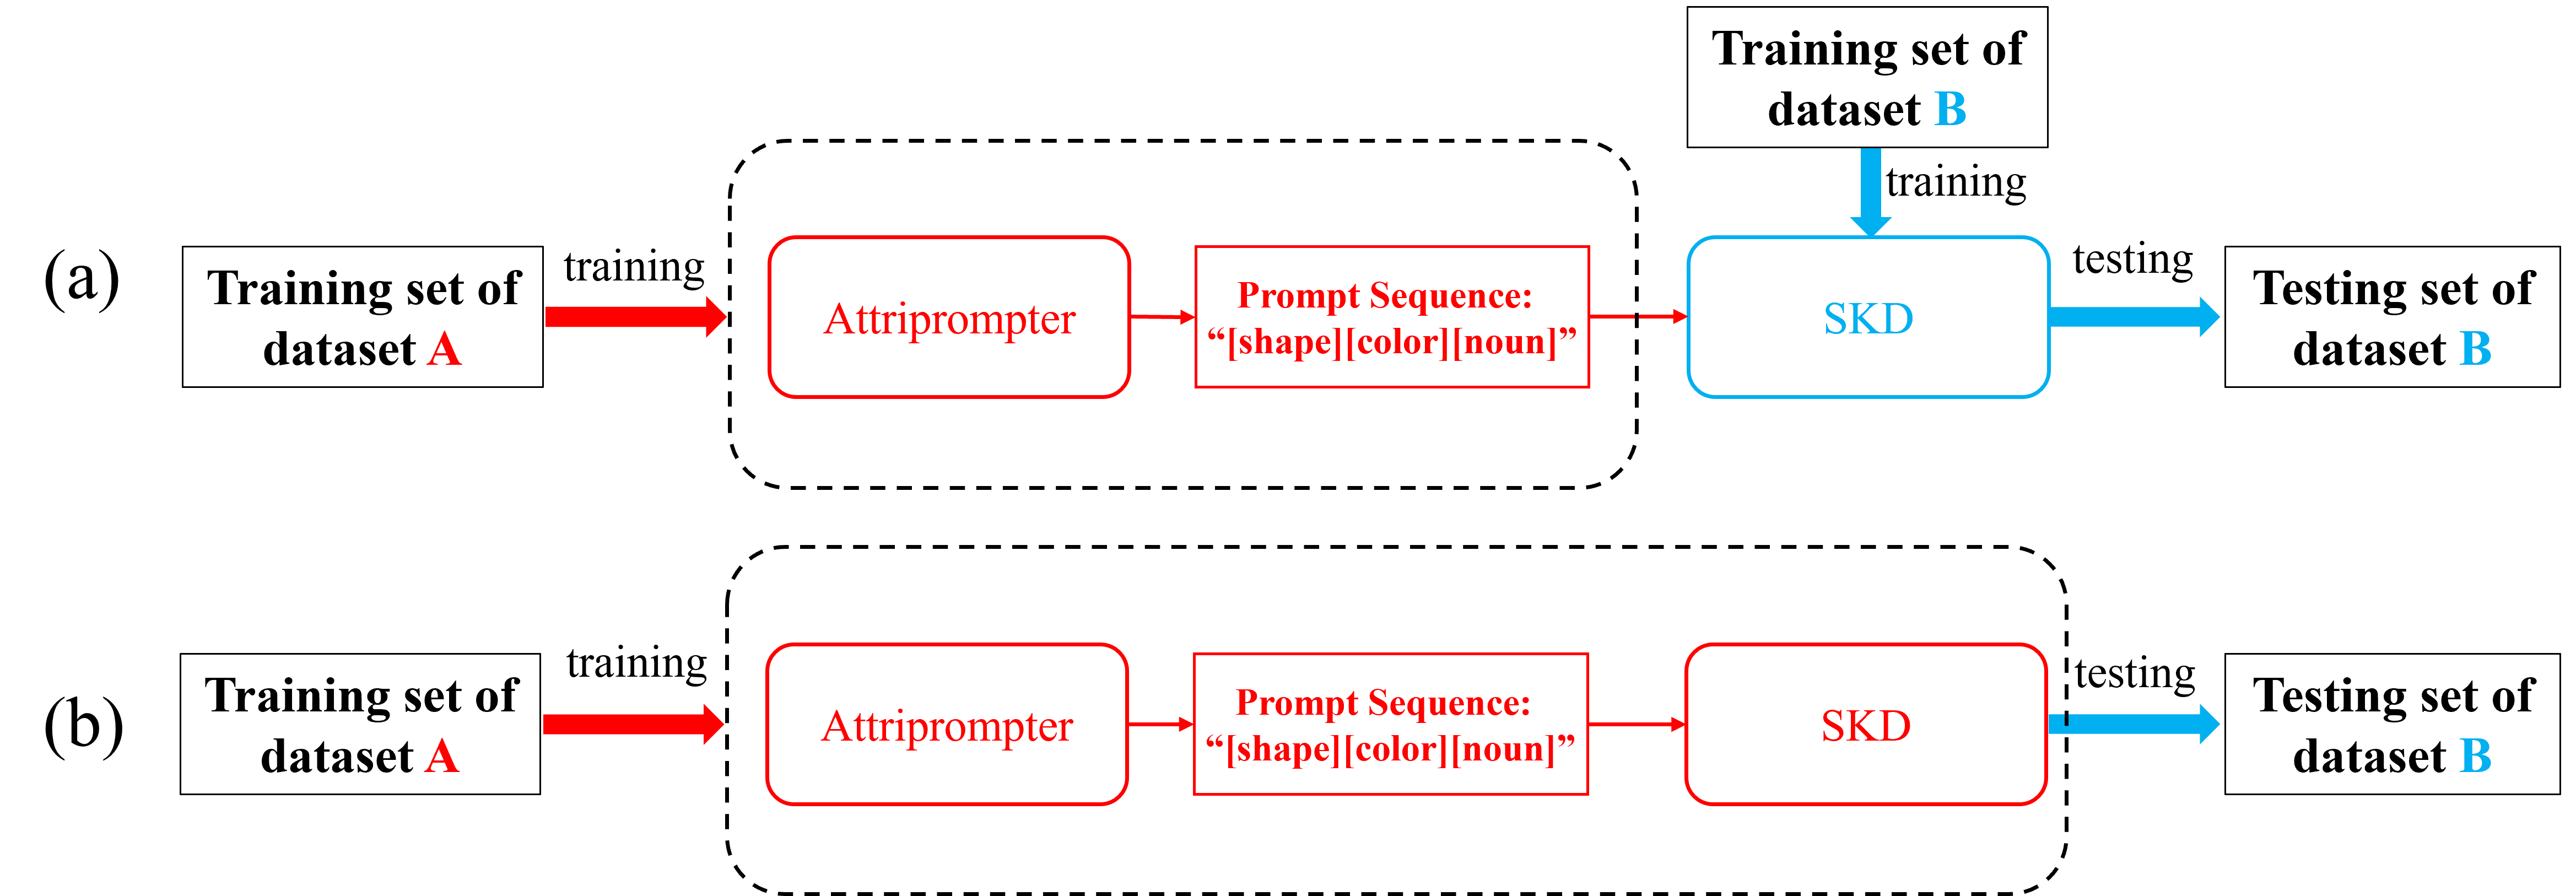
\includegraphics[width=\linewidth]{chapters/PAPERS/nucleiprompter__TMI_final_version/xu5.png}
\caption{两组跨域实验示意图。(a) 验证 AttriPrompter 的跨域能力；(b) 验证完整系统的 domain shift 性能。数据集 A 和数据集 B 分别表示源域和目标域。}
\label{fig:attrip_cross_domain}
\end{figure}

\subsection{AttriPrompter 的跨域能力}

表~\ref{tab:attrip_cross_capacity} 展示提示生成数据集和 SKD/测试数据集不同时的结果。使用 MoNuSeg 生成提示并在 MoNuSeg 上测试时，mAP 为 0.425；使用 CoNSeP 生成提示、在 MoNuSeg 上进行 SKD 和测试时，mAP 降至 0.405。反方向的结果也呈现类似趋势。说明提示属性具有一定的跨域迁移能力，但不同数据集在染色颜色和细胞核形态上的差异仍会造成性能下降。

\begin{table}[t]
\caption{AttriPrompter 跨域能力验证。}
\label{tab:attrip_cross_capacity}
\begin{center}
\resizebox{0.9\columnwidth}{!}{
\begin{tabular}{cccccc}
\toprule[1.5pt]
\textbf{用于生成提示的数据集} & \textbf{用于 SKD 和测试的数据集} & \textbf{mAP} & \textbf{AP50} & \textbf{AP75} & \textbf{AR} \\ \midrule[1.2pt]
\textbf{MoNuSeg} & \textbf{MoNuSeg} & 0.425 & 0.819 & 0.401 & 0.511 \\
\textbf{CoNSeP} & \textbf{MoNuSeg} & 0.405 & 0.759 & 0.400 & 0.480 \\ \midrule
\textbf{CoNSeP} & \textbf{CoNSeP} & 0.367 & 0.669 & 0.376 & 0.488 \\
\textbf{MoNuSeg} & \textbf{CoNSeP} & 0.339 & 0.669 & 0.324 & 0.441 \\ \bottomrule[1.5pt]
\end{tabular}
}
\end{center}
\vskip -0.15in
\end{table}

该结果表明，AttriPrompter 生成的属性并非只对单个数据集有效。即使提示生成域与测试域不同，常见的形状和颜色词仍然能够保留一定的检测能力；但若希望获得最佳性能，提示生成所依据的无标注图像应尽量接近目标测试域。

\subsection{完整系统的 domain shift}

第二组实验在源域上生成提示并完成 SKD，然后在不同目标域上测试。表~\ref{tab:attrip_domain_shift} 中的 ``MoNuSeg $\rightarrow$ CoNSeP'' 表示源域为 MoNuSeg、目标域为 CoNSeP；反向箭头表示相反方向。标准零样本方法不进行跨域训练，使用面向目标域手工设计的提示，作为灰色背景基线。

\begin{table}[t]
\caption{完整框架的 domain shift 实验。箭头表示源域到目标域的方向；标准零样本方法不执行跨域过程。最优结果以粗体表示。}
\label{tab:attrip_domain_shift}
\begin{center}
\resizebox{0.96\columnwidth}{!}{
\begin{tabular}{ccccccccc}
\toprule[1.5pt]
 & \multicolumn{4}{c}{\textbf{MoNuSeg $\rightarrow$ CoNSeP}} & \multicolumn{4}{c}{\textbf{CoNSeP $\rightarrow$ MoNuSeg}} \\ \cmidrule(r){2-5} \cmidrule(r){6-9}
\multirow{-2}{*}{\textbf{方法}} & \textbf{mAP} & \textbf{AP50} & \textbf{AP75} & \textbf{AR} & \textbf{mAP} & \textbf{AP50} & \textbf{AP75} & \textbf{AR} \\ \midrule
\rowcolor{lightgray}
\textbf{标准零样本（人工提示）} & 0.062 & 0.131 & 0.055 & 0.111 & 0.151 & 0.259 & 0.166 & 0.210 \\
\textbf{SSNS (2020)\cite{sahasrabudhe2020self}} & 0.122 & 0.310 & 0.101 & 0.274 & 0.111 & 0.204 & 0.115 & 0.169 \\
\textbf{VL-PLM (2022)\cite{zhao2022exploiting}} & 0.118 & 0.307 & 0.097 & 0.275 & 0.096 & 0.175 & 0.108 & 0.133 \\
\textbf{VLPM-NuD (2023)\cite{wu2023zeroshot}} & 0.152 & 0.389 & 0.080 & 0.257 & 0.173 & 0.250 & 0.171 & 0.225 \\
\textbf{AttriPrompter} & 0.082 & 0.182 & 0.061 & 0.124 & 0.168 & 0.287 & 0.175 & 0.199 \\
\textbf{AttriPrompter + SKD} & \textbf{0.178} & \textbf{0.439} & \textbf{0.112} & \textbf{0.285} & \textbf{0.260} & \textbf{0.594} & \textbf{0.178} & \textbf{0.356} \\ \bottomrule[1.5pt]
\end{tabular}
}
\end{center}
\end{table}

与同域结果相比，所有方法在 domain shift 下均出现不同程度的性能下降，但 AttriPrompter + SKD 仍取得最佳结果。源域提示在目标域中仍能发挥作用，可能是因为不同 H\&E 数据集之间具有一定共性，而自动生成过程倾向于选择自然语言中较常见的形状和颜色词。相反，人工提示容易加入 GLIP 预训练语料中覆盖不足的医学描述，因此在跨域条件下不一定更有效。SKD 在跨域场景中的收益说明，学生网络不仅能够修正初始检测框，还能通过源域伪标签学习较稳定的目标级结构表示。

\section{讨论与局限性}

本章实验说明，视觉语言模型应用于医学图像时，提示并非简单的类别名称替换。对于细胞核这类密集、相似且尺度较小的目标，形状和颜色属性提供了比医学名词更直接的视觉线索；程度增强可以扩大细粒度描述空间；相关性排序则利用了 GLIP 对输入序列顺序的敏感性。三者共同构成了从目标域图像到文本提示的自动化桥梁。

同时，SKD 解决的是“如何利用初始提示结果继续改善检测”的问题，而不是替代提示生成。伪标签实验表明，如果初始伪标签缺乏准确的目标语义，单纯增加自训练轮次并不能保证得到理想结果。知识蒸馏损失能够帮助学生网络保留 GLIP 的目标级知识，但最终结果仍受初始伪标签质量、学生网络结构和训练轮次影响。

本章仍存在以下局限。第一，当前属性生成主要关注形状和颜色，尚未充分利用纹理、染色强度、细胞核内部结构和空间上下文等信息。第二，SKD 需要多轮学生网络训练，计算开销较高，在大规模全视野图像上仍需要进一步优化。第三，domain shift 实验显示，提示和伪标签在跨域时会出现性能下降，说明当前方法还不能完全消除不同中心、设备和染色流程带来的域差异。后续研究可以从更丰富的属性生成、低成本的伪标签更新以及面向病理图像的域泛化策略三个方向继续改进。

\section{本章小结}

本章研究了结合自动属性提示和自训练知识蒸馏的无标注零样本细胞核检测方法。首先，通过提示实证分析发现，细粒度语义和合理的提示顺序能够显著影响 GLIP 的零样本预测。随后提出 AttriPrompter，从无标注病理图像中自动生成形状和颜色属性，并通过同义增强、程度增强和相关性排序构造最终提示序列。针对密集细胞核造成的漏检、误检和目标重叠问题，进一步构建 SKD 框架，以 GLIP 为教师、检测专用网络为学生，通过特征蒸馏和多轮自训练优化预测结果。

在 MoNuSeg 和 CoNSeP 上的实验表明，AttriPrompter 在无监督方法中取得了较好的综合性能；组件消融验证了程度增强和相关性排序的作用；伪标签和知识蒸馏实验说明，初始提示质量与 GLIP 先验知识迁移是性能提升的关键；不同学生网络和跨域实验则证明了该框架具有一定的结构泛化和域迁移能力。本章为后续章节进一步研究视觉文本化提示和跨域医学图像分析提供了基础。

% 工作三：VisTex
\chapter{VisTex：面向目标级视觉语言模型的视觉文本化图像提示}

\section{研究背景与问题提出}
目标检测方法通常依赖大规模标注数据\cite{redmon2016you,ren2016faster}，在稀缺场景（如长尾类别、专业领域与医学影像）中往往难以获取足够标注。因此，少样本目标检测（Few-shot Object Detection, FSOD）\cite{wang2019metadet,Qiao_2021_defrcn2}成为重要研究方向。近年来，视觉语言预训练模型（VLMs）通过海量图文对学习具有较强泛化能力的跨模态表示，使得“以文本提示进行零样本迁移”成为可能。然而，医学图像与专业领域的下游任务仍存在三类典型困难：其一，下游类别在预训练语料中覆盖不足；其二，文本提示的描述粒度有限，容易产生语义偏置与遗漏；其三，细粒度目标往往共享相近的文本描述，仅靠文本难以区分\cite{xu2023mqdet,du2022learning}。

目标级视觉语言模型（Object-level Vision-Language Models, OVLMs）\cite{li2022glip,dou2022fiber,liu2023groundingdino}以 GLIP\cite{li2022glip} 为代表，利用 grounding 数据与多尺度/多阶段跨注意力结构建立了更强的\textbf{目标级图文对齐}，在零样本检测中显著优于 CLIP\cite{radford2021clip} 等图像级 VLM。然而，如何在\textbf{不破坏 OVLM 预训练的图文对齐}前提下，把下游任务中少量支持样本（support images）所包含的视觉语义注入到提示推理过程，仍然是一个关键难题。

\section{动机：引入下游视觉语义而不破坏图文对齐}
现有基于 VLM 的 FSOD 方法通常通过\textbf{微调原模型权重}或\textbf{引入额外可学习结构}来利用支持图像信息，但在少量目标域数据下，这两类做法都可能导致原有的目标--文本相似度分布发生偏移，从而损害源域对齐并削弱泛化能力。更进一步地，许多 OVLM（如 GLIP 与 GroundingDINO）本质上是\textbf{“仅支持文本提示”的模型}，由于结构设计限制，缺少对图像提示（image prompting）的原生支持\cite{li2022glip,liu2023groundingdino}。

图像提示为解决上述问题提供了一条思路：用支持图像作为提示，与文本提示一起为下游推理提供语义引导\cite{luddecke2022clipseg,xu2023mqdet}。然而，现有代表方法 MQ-Det\cite{xu2023mqdet} 通过在文本编码器内部额外引入可学习跨注意力模块来实现“图像调制文本”，它主要对现有文本 token 进行重加权，而非直接引入新的视觉信息；同时，新引入的结构也可能进一步偏置 OVLM 的预训练对齐。

基于此，本章提出 VisTex-OVLM：通过\textbf{视觉文本化（visual textualization）}将支持图像投影到 OVLM 的\textbf{文本特征空间}，把支持样本以“文本 token”的形式直接并入提示序列，从而在不修改 OVLM 主体结构的前提下实现\textbf{直接图像提示}。

\section{任务定义与符号说明}
在经典 FSOD 设置中，存在基类数据集 $D_b$（类别集合 $C_b$）与新类数据集 $D_n$（类别集合 $C_n$），满足 $C_b\cap C_n=\emptyset$。在新类集合中，每个类别仅提供至多 $K$ 个带框标注实例（$K$-shot）。测试阶段中，提供少量标注的图像称为支持图像（support images），待预测的图像称为查询图像（query images）。在更一般的 GFSOD 设置中，测试类别集合为 $C_b\cup C_n$，要求模型在新类上提升的同时保持基类性能。

对 OVLM 的多尺度/多阶段编码过程，记第 $i$ 个 stage 的中间视觉特征与文本特征分别为 $R^i$ 与 $P^i$，其中 $i=0,1,\ldots,L$。多尺度特征记为 $R^i=\left[R^{i,(j)}\right]_{j=0}^{M-1}$，其中 $M$ 表示尺度数。

\section{方法：VisTex-OVLM 视觉文本化框架}
图 \ref{fig:vistex_framework} 给出了 VisTex-OVLM 的整体流程。其核心由两部分组成：\textbf{多尺度视觉文本化模块（Multi-scale Textualizing Blocks, MSTB）}与\textbf{多阶段融合策略（Multi-stage Fusion, MSF）}。二者共同将支持图像映射为一个或多个\textbf{视觉文本化 token}，并与常规文本提示 token 拼接后直接输入\textbf{冻结的} OVLM，实现无需改动主干结构的图像提示推理。

\begin{figure}[t]
  \centering
  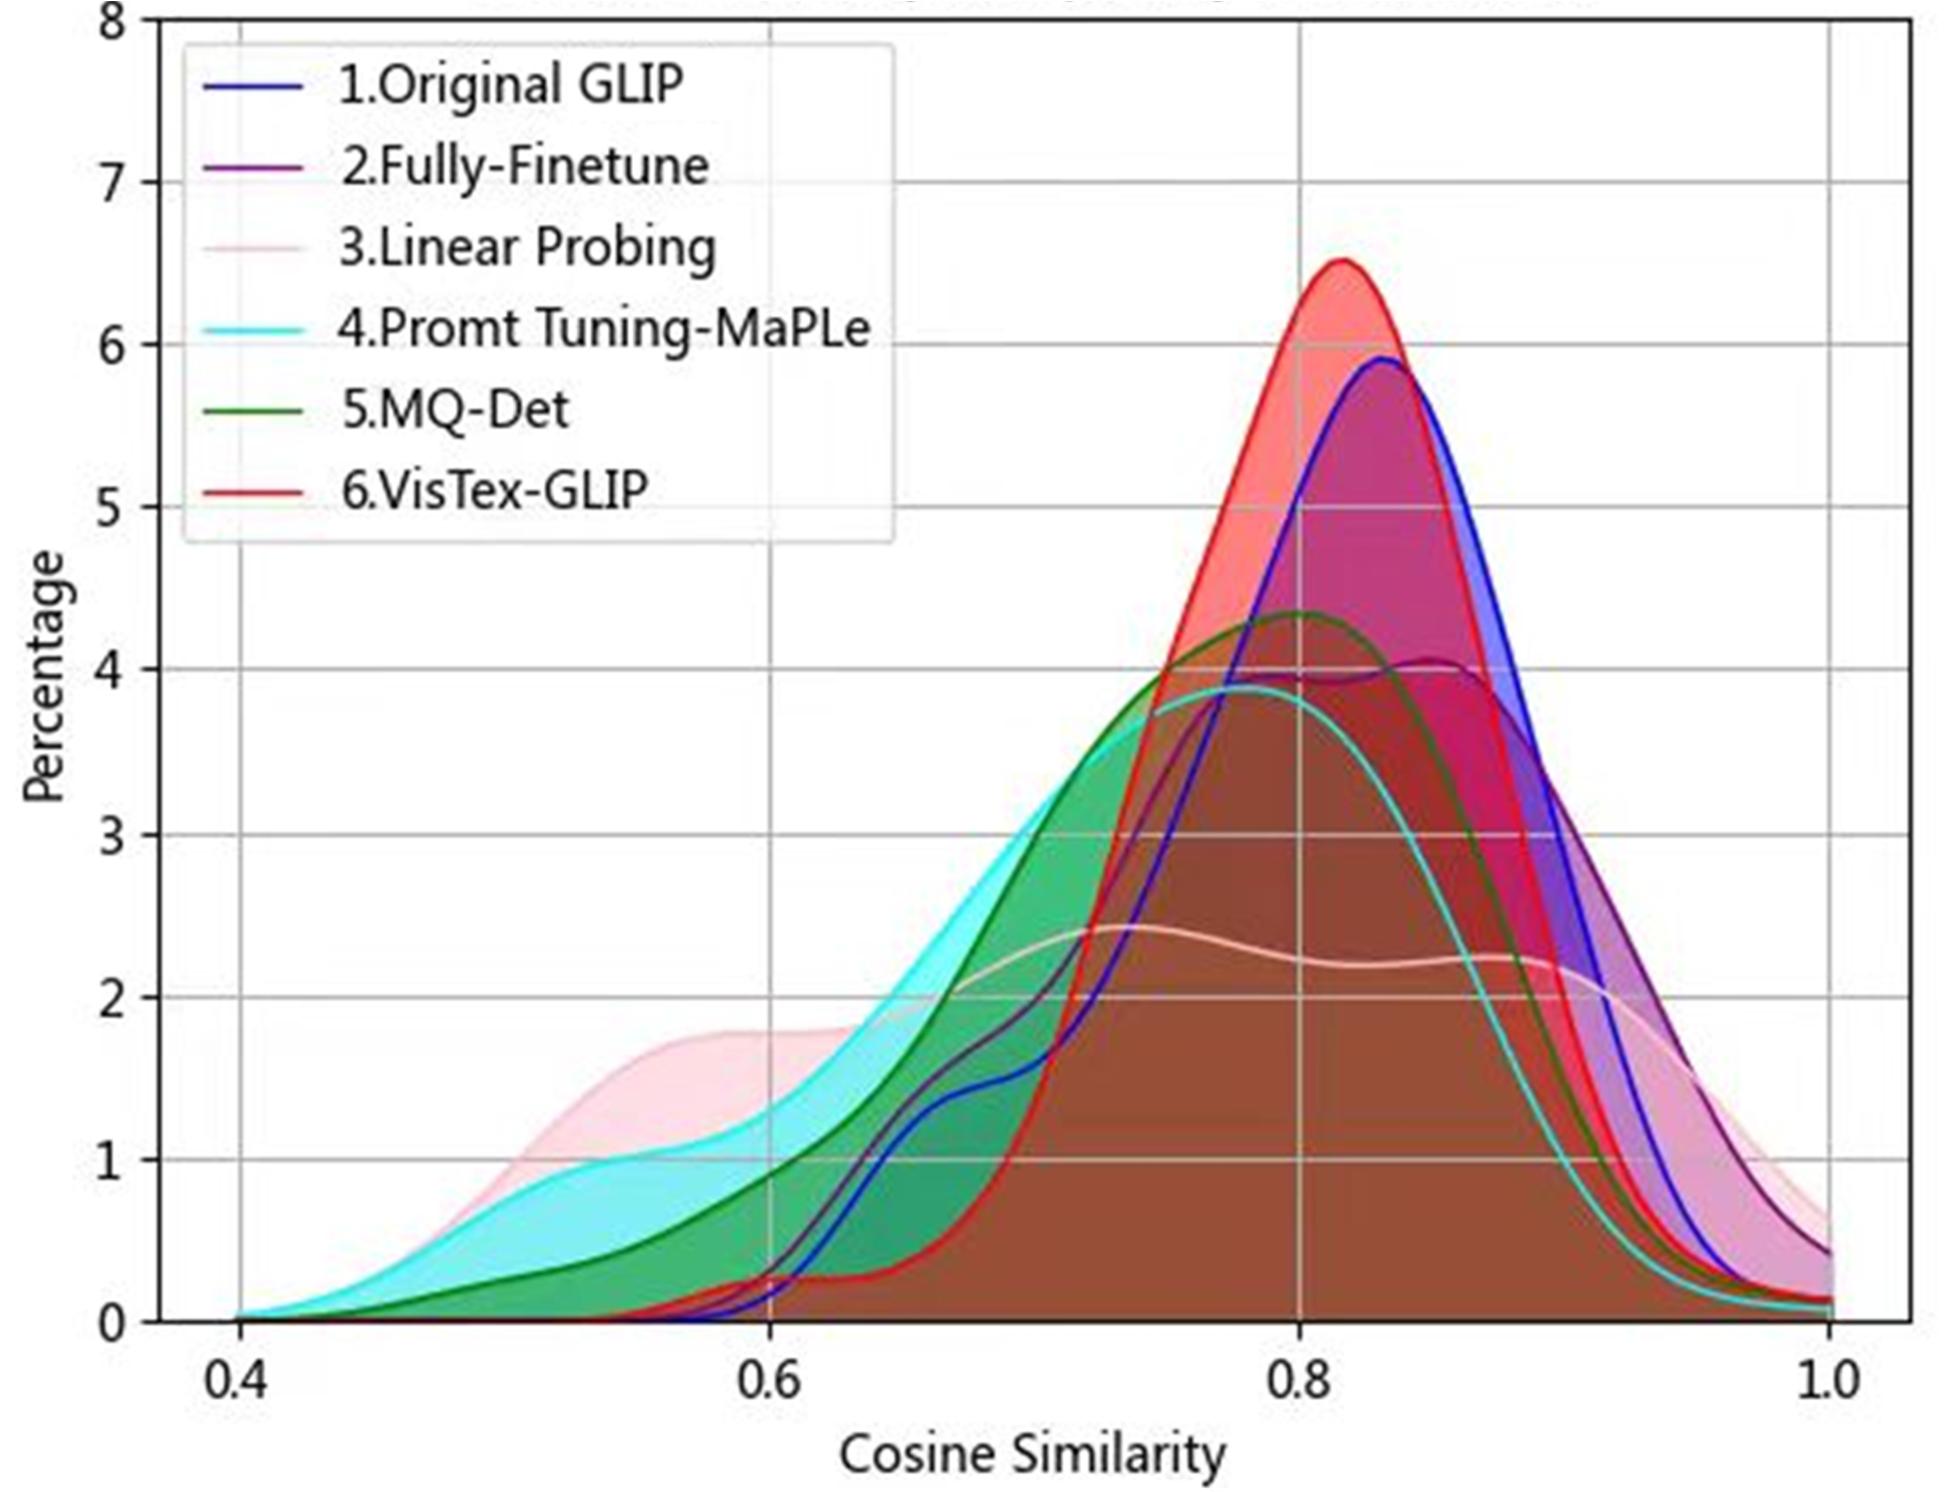
\includegraphics[width=0.96\linewidth]{chapters/PAPERS/VisTex_ICCV_ver/cosine1.png}
  \caption{不同迁移方式对 OVLM 源域图文对齐的影响。在有限目标域数据下，结构或权重的修改会使源域 object--text 相似度分布发生偏移，从而部分破坏预训练对齐。}
  \label{fig:vistex_cosine}
\end{figure}

\begin{figure}[t]
  \centering
  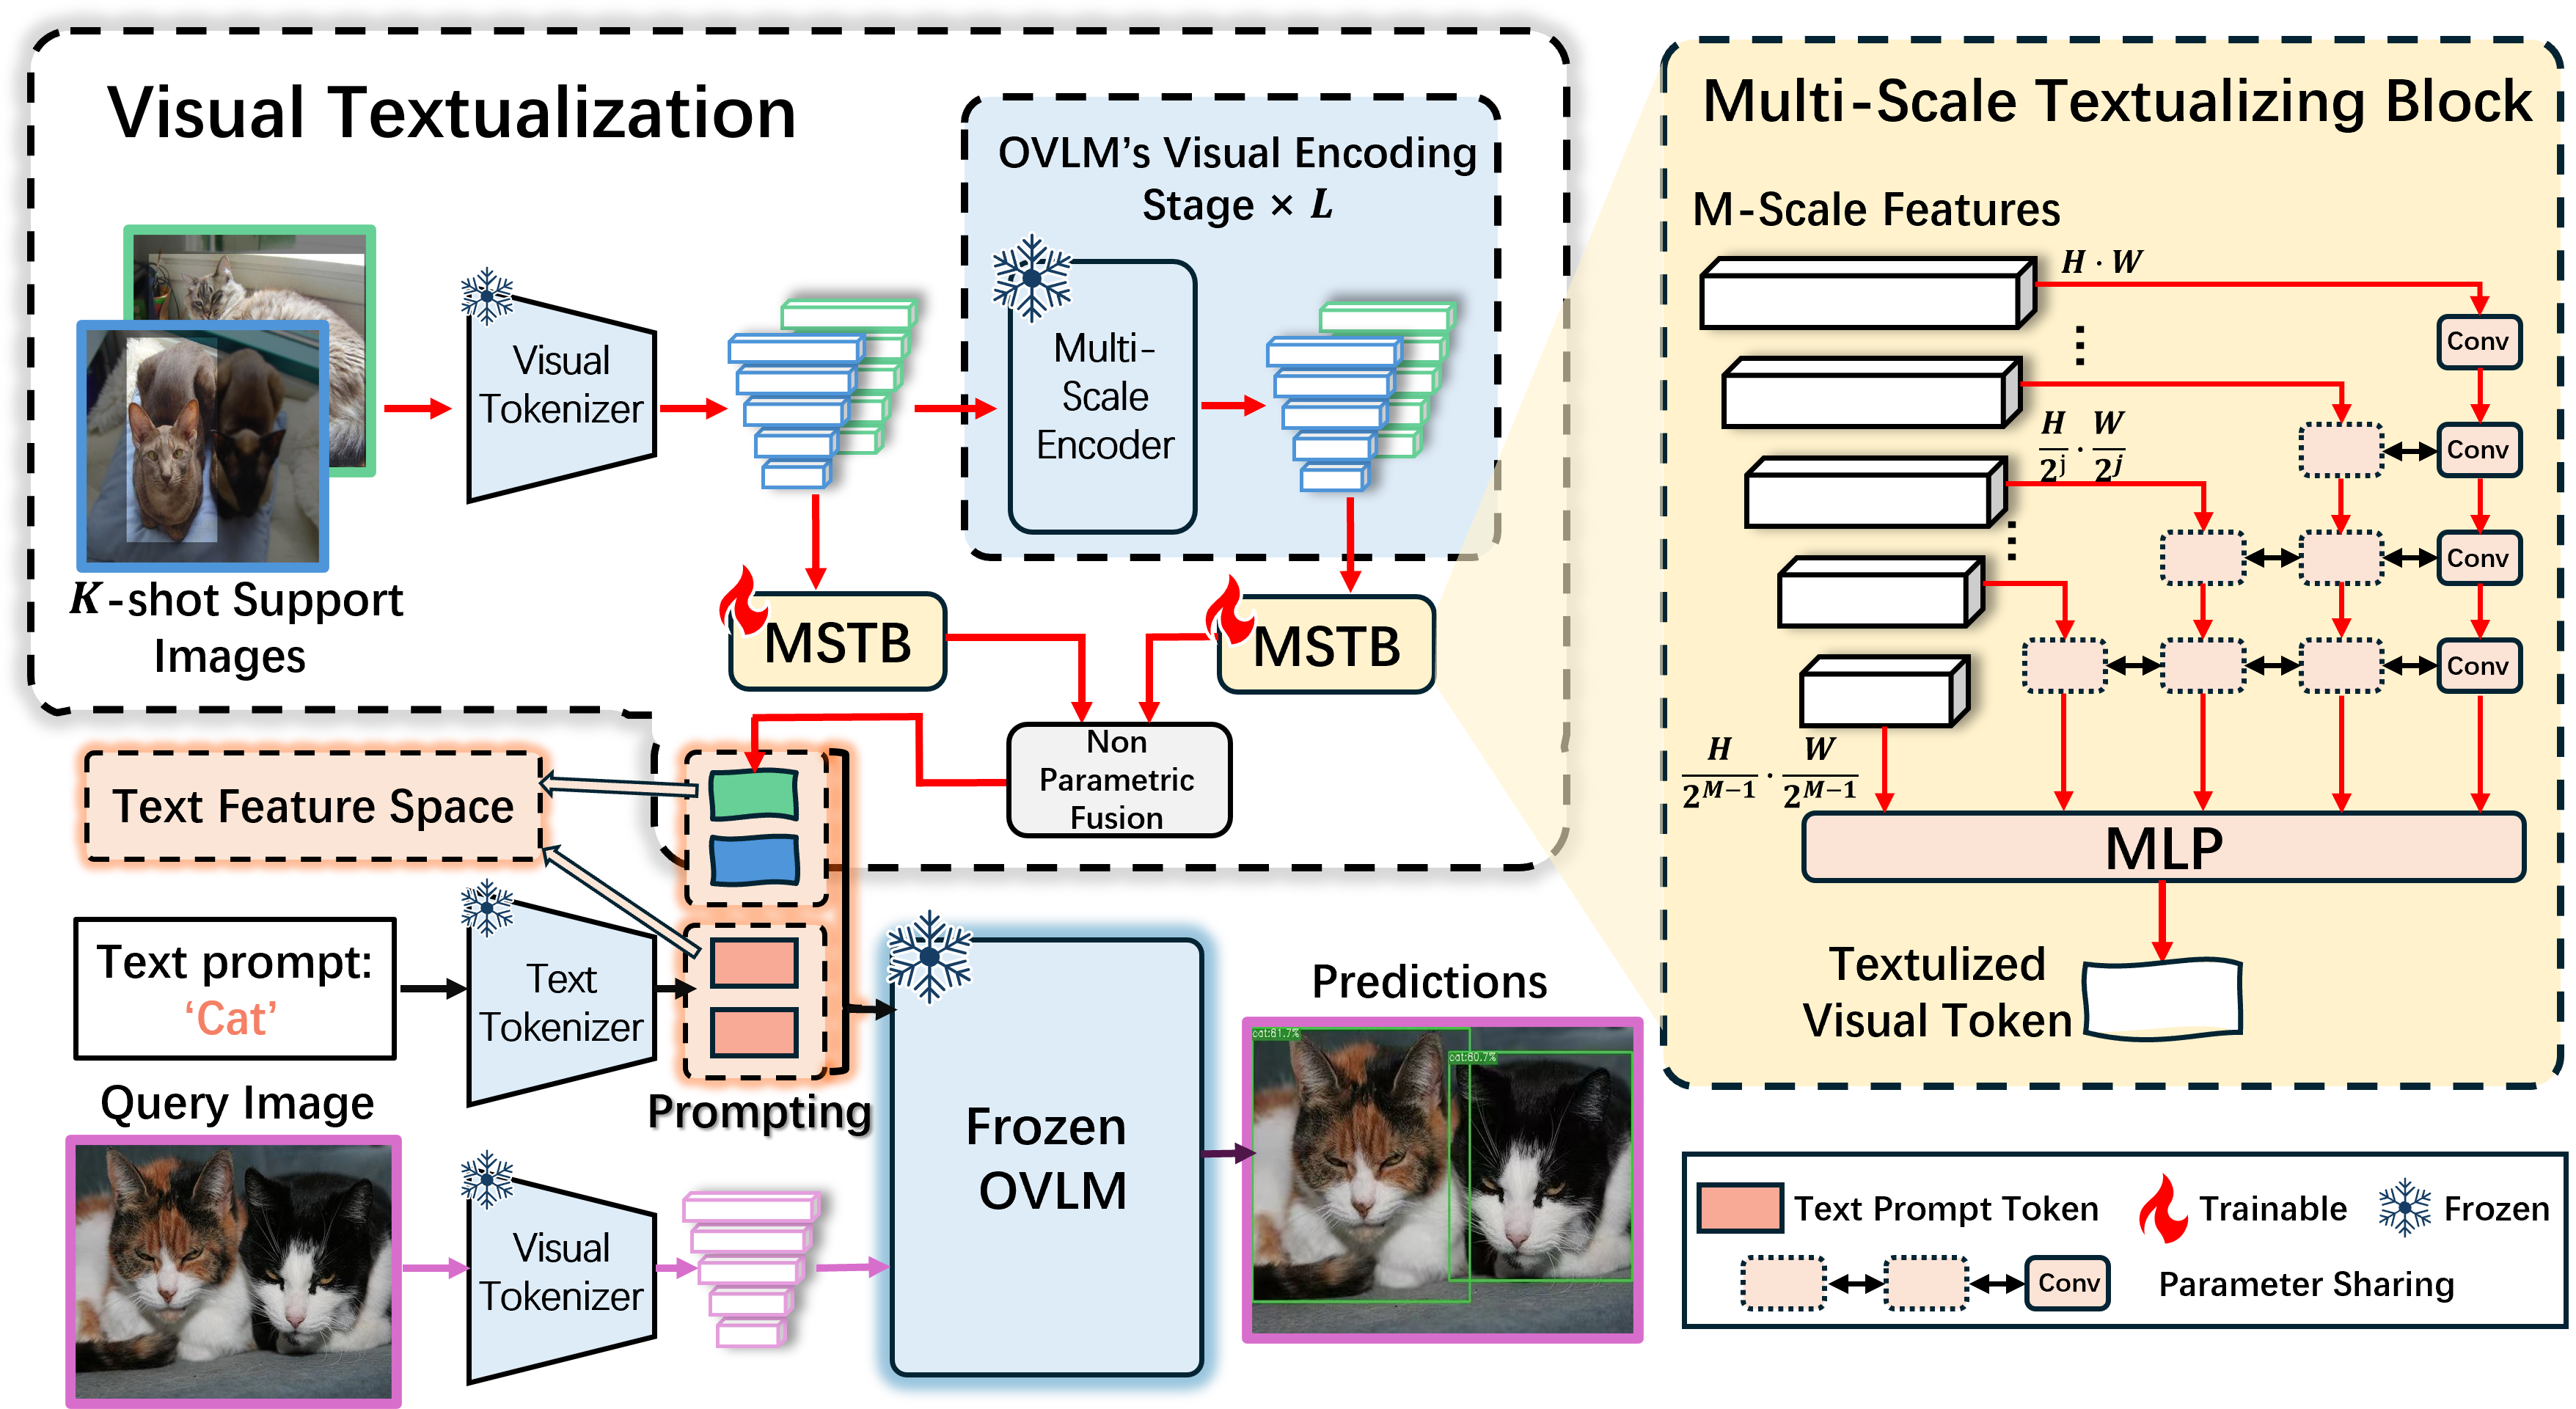
\includegraphics[width=\linewidth]{chapters/PAPERS/VisTex_ICCV_ver/method.png}
  \caption{VisTex-OVLM 框架示意。通过 MSTB 与 MSF 将支持图像投影到 OVLM 的文本特征空间，生成视觉文本化 token，并与文本提示共同驱动未修改的 OVLM（如 GLIP\cite{li2022glip}、GroundingDINO\cite{liu2023groundingdino}）完成少样本检测。}
  \label{fig:vistex_framework}
\end{figure}

\subsection{图像提示工程（Image Prompt Engineering）}
由于检测属于密集预测任务，支持图像中同时包含目标、背景及其它干扰物体。为最大化利用少样本标注，本章采用图像提示工程：结合支持图像中的目标框信息，对框外区域进行模糊化处理，使得支持图像更聚焦于目标实例\cite{luddecke2022clipseg}。

\subsection{多尺度视觉文本化（MSTB）}
给定提示工程后的支持图像 $x_S$，使用冻结的 OVLM 视觉编码器提取各 stage 的多尺度特征 $R^i_S=\left[R_S^{i,(j)}\right]_{j=0}^{M-1}$。MSTB 的目标是将不同尺度的视觉特征统一聚合，并映射到文本特征维度，从而得到 stage 级的视觉文本化特征 $\widetilde{P^i_S}$。

为高效共享跨尺度知识并降低训练成本，MSTB 采用参数共享策略：对除最小尺度以外的各尺度特征使用共享的下采样卷积逐级压缩到同一空间分辨率，拼接后再用 MLP 映射到文本空间，形式化为：
\begin{equation}
\begin{aligned}
    \widetilde{R^{i,(j)}_S} = \left\{
    \begin{array}{ll}
    \left( \prod_{j}^{M-2} \operatorname{Conv}_{\text{down}}^{i,(j)}\right) \left( R^{i,(j)}_S \right), & \text{if } j \neq M-1 \\
    R^{i,(j)}_S, & \text{if } j = M-1
    \end{array}
    \right.
\end{aligned}
\label{eq:vistex_downsample}
\end{equation}
\begin{equation}
    \widetilde{R^i_S} = \left[ \widetilde{R^{i,(j)}_S} \right]_{j=0}^{M-1},
\label{eq:vistex_concat}
\end{equation}
\begin{equation}
    \widetilde{P^i_S} = \operatorname{MLP}^i \left( \widetilde{R^i_S} \right).
\label{eq:vistex_mlp}
\end{equation}

\subsection{多阶段融合（MSF）}
OVLM 的多阶段编码对应着多阶段的跨模态对齐过程。为充分利用这种对齐先验，本章进一步对各 stage 的 $\widetilde{P^i_S}$ 进行非参数融合，得到最终的视觉文本化 token $\widetilde{P_S}$：
\begin{equation}
    \widetilde{P_S} = \operatorname{MSF} \left( \{ \widetilde{P^i_S}\}_{i=0}^L \right).
\label{eq:vistex_msf}
\end{equation}
由于 MSF 采用非参数操作（如跨 stage 的 max pooling），因此在不引入额外参数的情况下即可利用 OVLM 的多阶段对齐能力。

\subsection{直接支持图像提示（Direct Image Prompting）}
得到 $\widetilde{P_S}$ 后，将其与文本提示 $t$ 经 BERT 编码得到的 token 直接拼接，构成输入 OVLM 的提示序列：
\begin{equation}
    P^0 = \left[ \operatorname{BERT}\left(t\right), \widetilde{P_S} \right].
\label{eq:vistex_prompt_1shot}
\end{equation}
对于 $K$-shot 设置，为保持每个 shot 的独立性，直接拼接多个视觉文本化 token：
\begin{equation}
    P^0 = \left[ \operatorname{BERT}\left(t\right), \widetilde{P_{S_1}}, \cdots, \widetilde{P_{S_K}} \right].
\label{eq:vistex_prompt_kshot}
\end{equation}
在训练阶段，仅更新 MSTB 的参数，OVLM 主体保持冻结；训练完成后，MSTB 可直接对新类支持样本进行视觉文本化，从而在不微调 OVLM 的条件下完成少样本检测。

\section{实验设置与结果分析}
本章遵循标准 FSOD 协议\cite{wang2020frustratingly,zhang2022metaDETR1}在 PASCAL VOC\cite{everingham2010pascalvoc} 与 MSCOCO\cite{lin2014microsoftCOCO} 上评估方法，并进一步在 LVIS\cite{gupta2019lvis}、ODinW\cite{li2022odinw} 以及多个医学数据集（如 MoNuSeg\cite{kumar2017dataset}、CoNSeP\cite{graham2019hover} 等）上验证开放集迁移能力。
（1）\textbf{标准 FSOD/GFSOD 基准。} VisTex-OVLM 在 PASCAL VOC 与 MSCOCO 的多种 shot 设置下取得了显著提升，并在兼顾 base/novel 类别的 GFSOD 设置中保持了对基类的稳定识别能力。为便于在学位论文中呈现关键结论，这里给出 GFSOD 代表性结果（MSCOCO 10-shot/30-shot）。

\begin{table}[t]
    \centering
    \resizebox{0.8\linewidth}{!}{
    \begin{tabular}{ccccccc}
    \hline
    \multicolumn{1}{c|}{} & \multicolumn{3}{c|}{\textbf{10-shot}} & \multicolumn{3}{c}{\textbf{30-shot}} \\ \cline{2-7} 
    \multicolumn{1}{c|}{\multirow{-2}{*}{\textbf{Method}}} & \textbf{AP} & \textbf{bAP} & \multicolumn{1}{c|}{\textbf{nAP}} & \textbf{AP} & \textbf{bAP} & \textbf{nAP} \\ \hline
    \multicolumn{7}{c}{\textbf{non-VLM-based}} \\ \hline
    \multicolumn{1}{c|}{\textbf{DiGeo \cite{ma2023digeo}}} & 32.0 & 39.2 & \multicolumn{1}{c|}{10.3} & 33.1 & 39.4 & 14.2 \\
    \multicolumn{1}{c|}{\textbf{DE-VIT-L \cite{zhang2023devit}}} & 30.6 & 29.4 & \multicolumn{1}{c|}{34.0} & 30.6 & 29.5 & 34.0 \\ \hline
    \multicolumn{7}{c}{\textbf{VLM-based}} \\ \hline
    \multicolumn{1}{c|}{\textbf{FM-FSOD-L \cite{Han_2024_FM-FSOD}}} & 40.0 & 44.2 & \multicolumn{1}{c|}{27.7} & 43.1 & 45.2 & 37.0 \\
    \multicolumn{1}{c|}{\textbf{MQ-Det \cite{xu2023mqdet}}} & 46.9 & \textbf{46.5} & \multicolumn{1}{c|}{47.8} & 47.3 & 46.8 & 48.1 \\
    \multicolumn{1}{c|}{\textbf{VisTex-GLIP}} & \textbf{48.1} & 46.2 & \multicolumn{1}{c|}{\textbf{52.7}} & \textbf{48.9} & \textbf{47.2} & \textbf{53.6} \\ \hline
    \end{tabular}
    }
    \caption{MSCOCO 上的 GFSOD 结果。bAP/nAP 分别表示 base/novel 类别 AP。}
    \label{tab:vistex_gfsod}
\end{table}

（2）\textbf{定性可视化。} 图 \ref{fig:vistex_vis} 展示了在 COCO 上与多种代表方法的输出对比。

\begin{figure}[t]
  \centering
  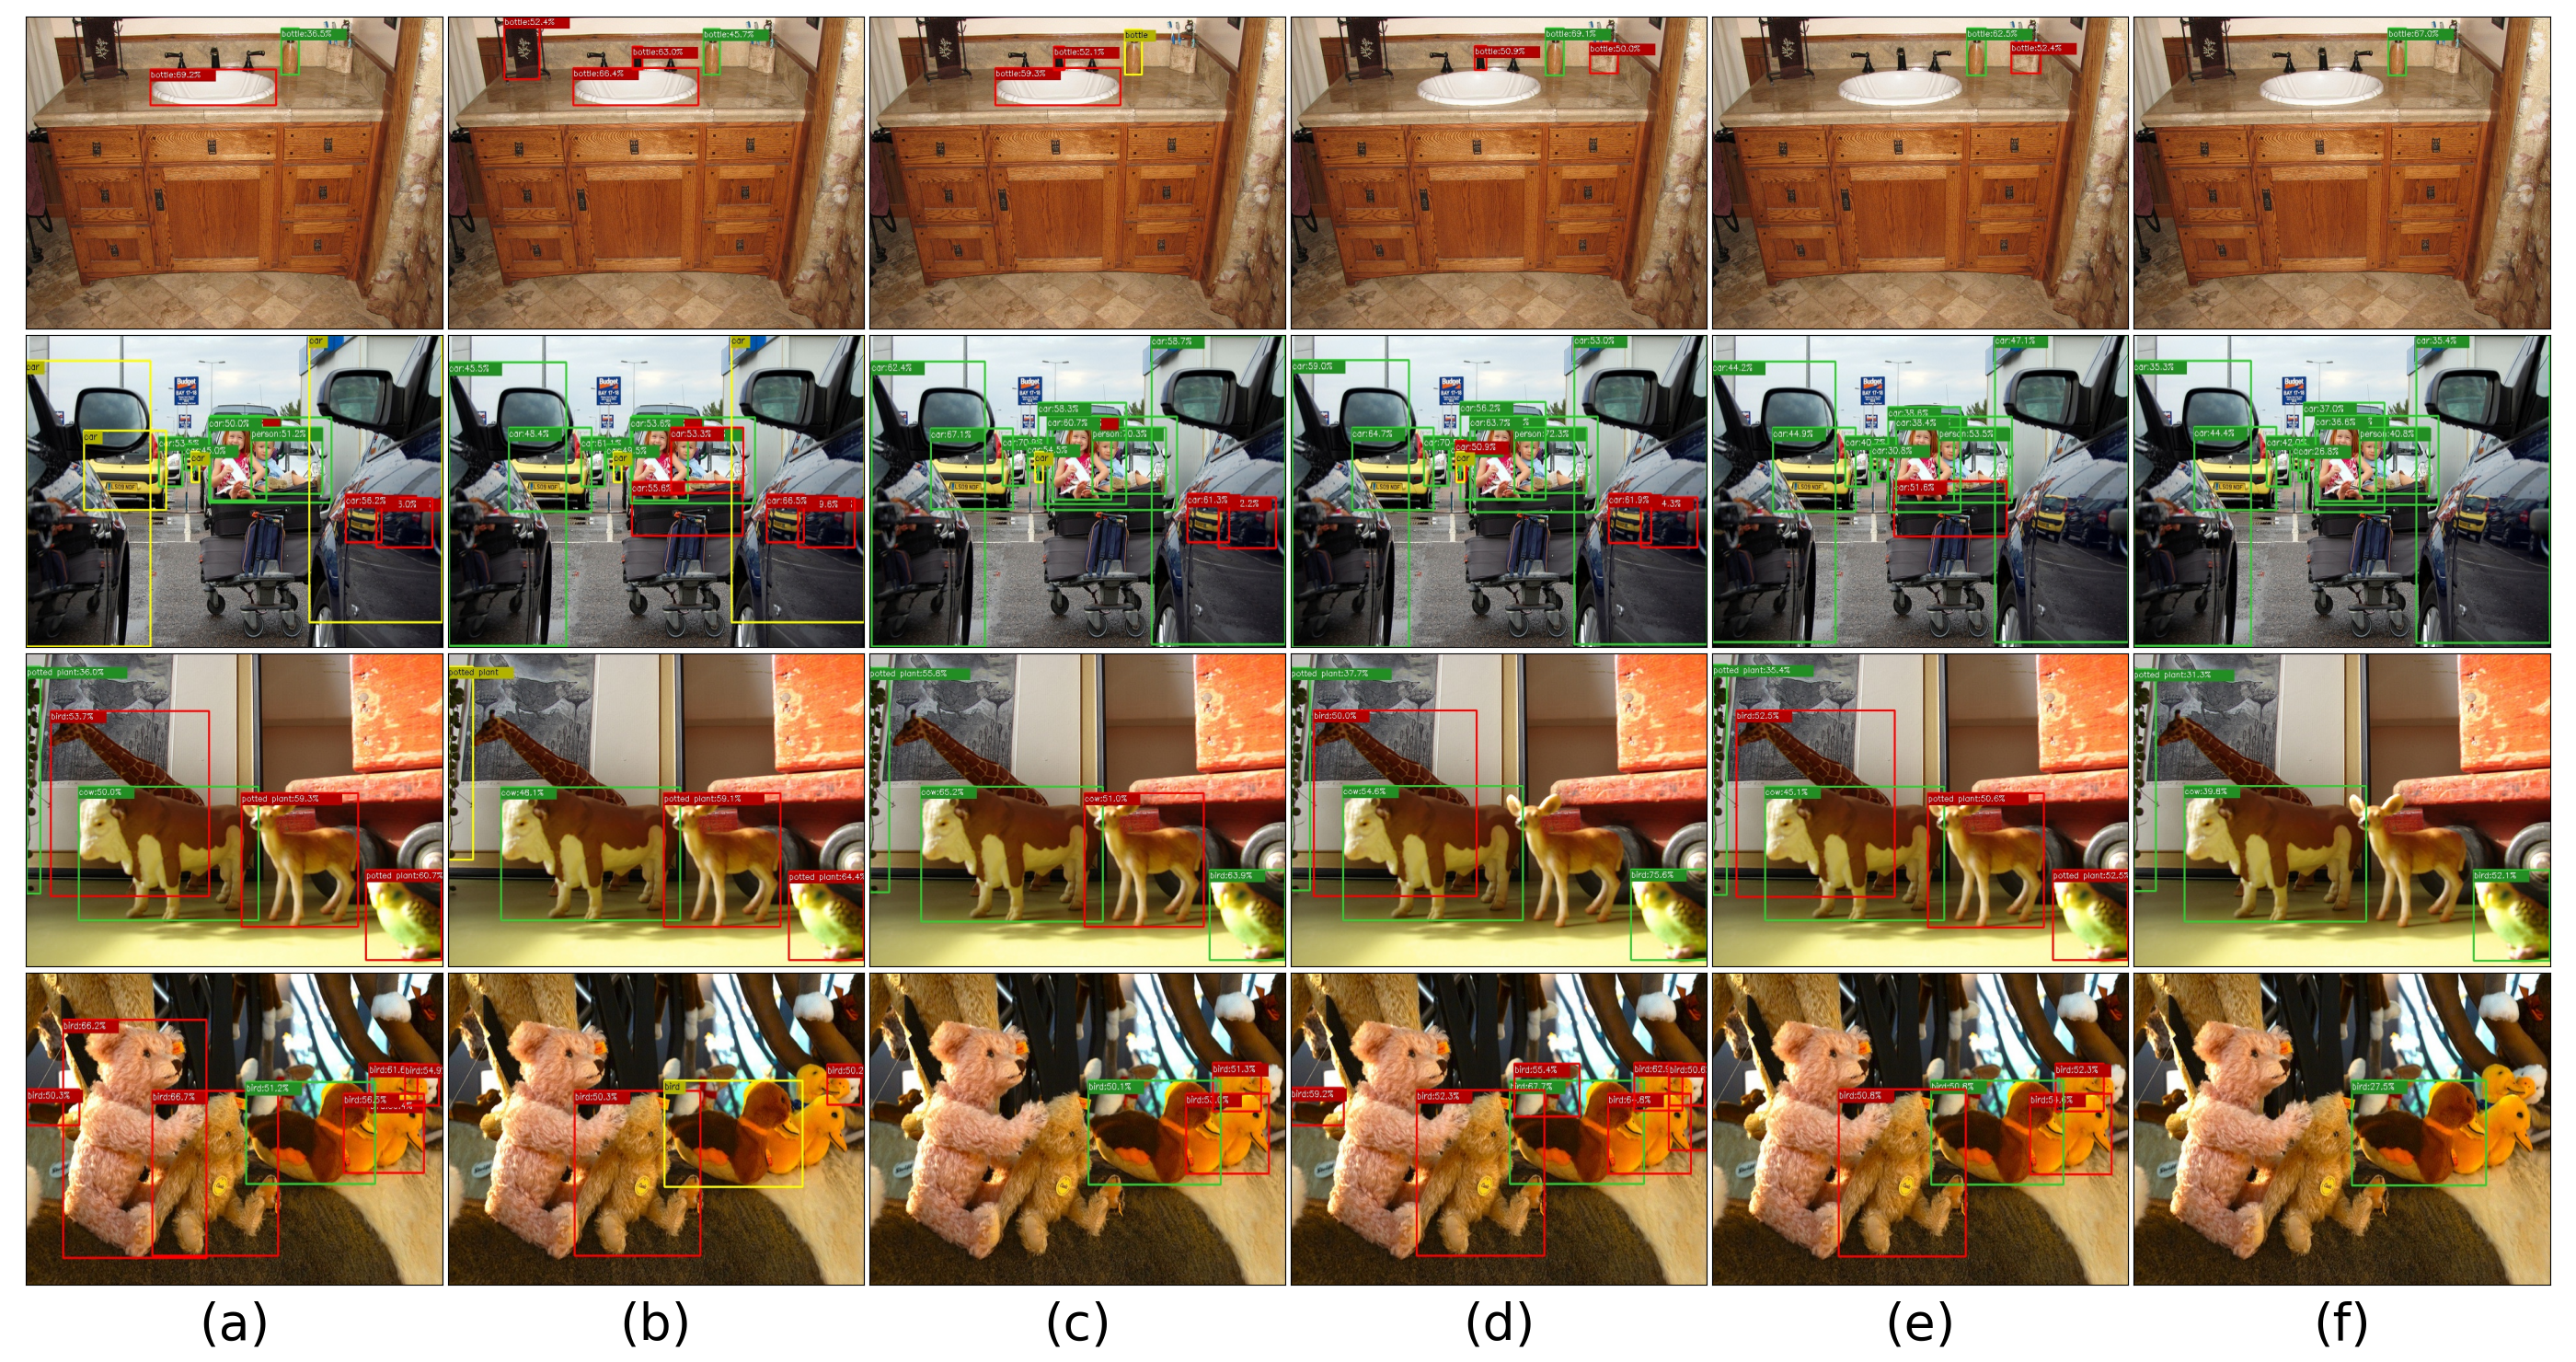
\includegraphics[width=\linewidth]{chapters/PAPERS/VisTex_ICCV_ver/vis_com.png}
  \caption{COCO 上的检测可视化对比。绿/红/黄框分别表示真阳性/假阳性/假阴性。}
  \label{fig:vistex_vis}
\end{figure}


\section{本章小结}
本章提出 VisTex-OVLM，通过视觉文本化将支持图像投影到 OVLM 的文本特征空间，使图像提示能够在不改动 OVLM 主体结构的情况下参与提示推理。借助 MSTB 的多尺度映射与 MSF 的多阶段融合，VisTex-OVLM 在标准少样本基准与开放集迁移设置中均取得了显著提升，验证了“以图像补充文本语义、且保持预训练图文对齐”的有效性。

% 工作四：Lung 数字病理应用
\chapter{面向肺鳞癌疗效评估的数字病理分析方法研究}

\section{引言}
新辅助免疫联合化疗已经成为可切除非小细胞肺癌的重要治疗方式，但术后病理评估仍面临两类相互关联的困难。NADIM、CheckMate-816、KEYNOTE-671、AEGEAN 和 CheckMate 77T 等临床研究从新辅助或围术期治疗角度一致支持免疫检查点抑制剂联合化疗在可切除非小细胞肺癌中的应用价值\cite{provencio2020nadim,forde2022checkmate816,wakelee2023keynote671,heymach2023aegean,cascone2024checkmate77t}；然而，治疗反应评估和风险分层仍面临挑战，尤其是未达到病理完全缓解的患者。CheckMate-816的长期随访结果显示，non-pCR患者约占全部接受治疗者的75\%，其5年总生存率仅为55.7\%，而pCR患者为95.3\%，凸显了这一主要人群的高风险属性。当前以 RVT 为代表的病理评估框架虽能提供重要预后信息。MPR 作为新辅助治疗后的替代终点已被系统提出，IASLC 也进一步规范了切除标本的病理评估口径\cite{hellmann2014mpr,travis2020iaslc}。
RVT 能够反映肿瘤退缩程度，却不能完整表征新辅助免疫化疗后形成的肿瘤--免疫生态。尤其是肿瘤边界附近的中性粒细胞聚集与较大空间范围内的淋巴细胞浸润，可能分别代表局部免疫抑制和持续抗肿瘤免疫，但这些空间表型在常规病理实践中难以稳定量化。以RVT为代表的病理评估框架在临床使用时主要面临以下两个主要问题：
第一，残余活性肿瘤（residual viable tumor, RVT）需要病理医师在多张全切片图像（whole-slide image, WSI）上综合估计活性肿瘤、坏死和治疗后间质的比例，耗时较长且容易受到观察者经验和区域异质性的影响。第二，病理完全缓解（pathological complete response, pCR）和主要病理缓解（major pathological response, MPR）均以离散阈值概括连续的治疗反应谱，难以进一步区分具有残余肿瘤患者的术后风险。

此外，仅关注肿瘤消退的基于 RVT 的指标并不能完全捕捉新辅助免疫化疗引起的复杂的免疫-肿瘤相互作用。肿瘤微环境（TME）特征提供了额外的预后信息。免疫浸润的丰度或模式，包括中性粒细胞、淋巴细胞和基质反应，与肺癌的治疗敏感性和生存相关\cite{wu2024coldhot,teijeira2021il8,miao2024neutrophilsnsclc,hu2025neutrophilpd1}。先前的研究表明，富含淋巴细胞的“热”肿瘤与改善的免疫治疗反应相关\cite{wu2024coldhot}，而肿瘤相关的中性粒细胞则导致免疫逃避和不良预后\cite{teijeira2021il8,miao2024neutrophilsnsclc,hu2025neutrophilpd1}。然而，由于其劳动密集型性质和有限的重复性，这些微环境特征在病理实践中并未被常规量化，并且它们在新辅助免疫化疗环境中的预后相关性，特别是在肺鳞状细胞癌（LUSC）中，仍未得到充分定义。
基于人工智能 (AI) 的数字病理学的最新进展使得能够对全切片图像 (WSI) 中的 RVT 和 TME 特征进行可重复、高通量的量化。大规模弱监督 WSI 学习和数据高效多实例学习已经证明，切片级标签可以支持临床级病理分类与跨队列验证\cite{campanella2019clinical,lu2021clam,ilse2018attentionmil,li2021dsmil,shao2021transmil}；层级自监督学习与全切片基础模型进一步表明，联合建模局部细胞形态和全局组织上下文能够提高 WSI 表征的迁移性\cite{chen2022hipt,xu2024gigapath}；在非小细胞肺癌中，深度学习还可从常规 H\&E 图像预测组织学类型与部分分子改变\cite{coudray2018lung}。AI 衍生的 RVT 已证明与仅接受新辅助免疫治疗的患者的病理学家评估和预后价值高度一致\cite{dacic2024lcmc3}。然而，目前尚不清楚人工智能衍生的指标在新辅助免疫化疗（现在是主要的新辅助策略）的背景下是否保留预测效用，以及这些定量特征如何与淋巴结状态等关键临床变量相互作用。与此同时，越来越多的证据表明，TME 内肿瘤和基质免疫细胞的空间组成和组织可以使用基于深度学习的病理模型进行定量表征，并作为肺腺癌的独立预后因素\cite{wang2020compstaining,wang2019convpath}。值得注意的是，基于人工智能的全玻片分析仪能够识别癌症区域、间质和关键 TME 成分，包括肿瘤浸润淋巴细胞、成纤维细胞和内皮细胞，能够描绘 TKI 耐药后 EGFR 突变 NSCLC 的动态微环境变化，并预测随后对基于免疫疗法的治疗的反应\cite{bang2025egfrspatial}。这些发现强调了人工智能衍生的空间 TME 特征在告知免疫治疗反应方面具有更广泛的相关性，并促使它们整合到基于 RVT 的生存模型中，特别是对于非 pCR 人群。
因此，利用国家癌症中心的两个队列（NCC\_Cohort1 和 NCC\_Cohort2）的数据集以及山西省肿瘤医院（SXCH）和深圳肿瘤医院（SZCH）的其他外部队列的数据集，我们开发了一个多尺度 AI 驱动的病理学框架，该框架可以同时量化接受新辅助免疫化疗治疗的 LUSC WSI 中的 RVT 与瘤周免疫细胞密度。这种综合方法旨在加强术后风险分层，特别是非 pCR 患者，并为辅助治疗决策和临床监测提供更有生物学依据的基础。


本章以接受新辅助免疫化疗的肺鳞状细胞癌（lung squamous cell carcinoma, LUSC）患者为研究对象，建立一套模拟病理医师多尺度阅片过程的数字病理框架。该框架首先在 WSI 上识别肿瘤床、活性肿瘤、坏死和正常组织，计算连续的 AI-RVT；随后利用视觉语言基础模型完成多类细胞检测，并按细胞到肿瘤边界的距离构建空间免疫表型；最后分别评价 AI-RVT、单一空间细胞特征及联合免疫表型与无病生存（disease-free survival, DFS）和总生存（overall survival, OS）的关系。与直接输出生存风险的黑箱模型不同，本研究保留区域、细胞类别、空间距离和临床终点之间的对应关系，使每一级结果均可由病理医师追溯核验。

\section{肺鳞癌数字病理分析方法}
\subsection{研究目标与总体技术路线}
本章目标是把肺鳞癌新辅助治疗后病理评价转化为一条可复现的计算链：首先在 WSI 上识别肿瘤床、活性肿瘤、坏死与正常组织并计算连续 AI-RVT；随后利用渐进式视觉语言学习检测肿瘤及免疫--间质细胞；最后以肿瘤边界为参照构建距离分层的空间细胞密度，并分析这些图像指标与病理缓解及患者预后的关系。与单纯追求检测精度不同，该技术路线要求图像层输出能够稳定聚合到切片级和患者级，并能进入临床统计模型。

\subsection{多尺度区域分析与残余肿瘤量化}
病理医师通常先在器官和组织尺度定位病变，再在细胞尺度确认活性肿瘤。若感受野不足，模型难以像医师一样综合更大范围内的组织结构与细胞分布信息，从而对局部区域的细胞类型与病理状态作出可靠判断。为模拟这种“放大--缩小”的阅片过程，本研究以最小尺度图块为中心逐级扩展感受野，生成空间对齐的大尺度训练样本。不同尺度分别建立区域分类分支，并通过空间对齐保持中心位置一致，使尺度变化只改变上下文范围而不改变预测对象。推理时再融合各尺度证据，从而避免单一局部纹理主导区域判断。
推理时，各尺度模型独立输出四类区域得分，再依据对应尺度中病理区域的面积进行加权融合。设第 $s$ 张切片中活性肿瘤、治疗后间质性肿瘤床和坏死区域面积分别为 $A^{(s)}_{\mathrm{tumor}}$、$A^{(s)}_{\mathrm{bed}}$ 和 $A^{(s)}_{\mathrm{necrosis}}$，则切片级 RVT 表示为
\begin{equation}
R_s=\frac{A^{(s)}_{\mathrm{tumor}}}
{A^{(s)}_{\mathrm{tumor}}+A^{(s)}_{\mathrm{bed}}+A^{(s)}_{\mathrm{necrosis}}+\epsilon}.
\end{equation}
设患者共有 $S$ 张可用切片，其患者级 AI-RVT 为
\begin{equation}
R_{\mathrm{patient}}=\frac{1}{S}\sum_{s=1}^{S}R_s.
\end{equation}
这一连续值既可按 10\% 阈值转换为 MPR 标签，也可直接进入 Cox 模型。

\subsection{渐进式视觉语言细胞检测}
目标队列中的细胞精细标注数量有限，且不同公共病理数据集的标签空间并不一致。为避免直接在少量目标域样本上训练导致过拟合，本研究将模型适配拆分为三个连续过程，并严格区分公开病理数据预训练、目标域粗粒度适配和目标域细粒度精调。其核心思想是先学习跨数据集稳定的细胞形态与视觉语言对应关系，再逐步注入目标队列的染色风格、组织结构和细胞类别信息。

\subsubsection{公开医学病理数据预训练}
第一阶段使用 MoNuSAC、CCRCC 和 CoNSeP 等公开医学病理数据集进行多类细胞预训练。其中，MoNuSAC 与同类多器官核数据集为跨组织细胞核分割和分类提供了标准化训练基础\cite{verma2021monusac,gamper2019pannuke,graham2021lizard}。与直接把所有数据的类别编号拼接在一起不同，本研究首先将不同数据集中的类别名称统一映射到细胞语义空间，并将类别名称作为文本提示输入 GLIP 的语言分支。图像编码器负责提取细胞的形态、纹理和局部组织背景，语言编码器则提供可迁移的类别语义；检测头通过区域--文本匹配学习细胞区域与类别短语之间的对应关系。这样做的目的不是让模型记忆某一个数据集的染色或类别编号，而是使其在不同标注体系之间学习较稳定的细胞外观表示，为后续目标域适配提供病理视觉先验。

在实现上，过程一以 GLIP-L 的预训练参数作为基础初始化，并采用与后续目标域训练一致的检测框架和文本提示形式。公开数据预训练阶段主要承担两个作用：一是将自然图像中的开放词汇检测能力迁移到细胞和细胞核等医学目标；二是利用多个公开数据集的形态变化增加训练样本的覆盖范围，减弱模型对单一数据集染色风格和标注习惯的依赖。由于该阶段使用的是公开医学数据而非本研究队列的测试图块，因此不会直接泄漏目标测试图像的实例标注。

\subsubsection{目标域粗粒度适配}
第二阶段在 NCC\_Cohort1 的目标域 WSI 上继续训练。我们从 7 例患者的 WSI 中提取 1,318 个图块，使用 Tumor 和 Stromal 两类相对可靠的粗粒度区域标签进行域内适配。此时不急于加入所有细粒度细胞类别，而是先让图像编码器和检测头适应本研究队列的 H\&E 染色、组织背景、肿瘤--间质结构及图块尺度。这样可以避免在细粒度标注尚不充分时，把类别遗漏或边界不确定性过早传播到整个模型。

\subsubsection{目标域细粒度精调}
第三阶段从完整标注区域以重叠采样方式获得 938 个 $224\times224$ 图块，对 Tumor cell、Lymphocyte、Neutrophil、Eosinophil、Plasma Cell、Endothelial Cell、Fibroblast 和 Histiocyte 八类细胞进行精调；小于图块尺寸的区域采用黑色填充。另从测试数据中按相同策略选取 8 个图块用于检测性能评价。细粒度精调阶段使用高质量逐实例标注，重点优化类别判别、实例边界和密集细胞场景中的区域匹配关系。

\subsection{肿瘤周围细胞提取与空间密度}
对存在残余肿瘤的 WSI，选取面积最大的肿瘤区域作为代表灶，并沿其轮廓提取周边图块；未检测到活性肿瘤时，则以最大间质区域为中心提取半径为 5 个图块的邻域。细胞检测结果除类别和置信度外，还记录细胞相对最近肿瘤边界点的水平、垂直偏移 $(V_x,V_y)$，仅保留置信度不低于 0.5 的检测目标。细胞到边界的欧氏距离为
\begin{equation}
d=\sqrt{V_x^2+V_y^2}.
\end{equation}
由于 $V_x$ 和 $V_y$ 均限制在 $500\,\mu\mathrm{m}$ 内，可测最大距离约为 $707\,\mu\mathrm{m}$。因此，本研究以 $50\,\mu\mathrm{m}$ 为步长，在 $50$--$700\,\mu\mathrm{m}$ 范围内建立累积径向区域。若肿瘤边界周长为 $P$，向外扩张距离为 $d$，则依据 Minkowski--Steiner 展开公式估计周边面积
\begin{equation}
A(d)=P\,d+\pi d^2,
\end{equation}
相应细胞密度为
\begin{equation}
\rho_c(d)=\frac{N_c(d)}{A(d)},
\end{equation}
其中 $N_c(d)$ 为类别 $c$ 在距离 $d$ 内的检测数。患者级密度由其全部切片对应密度取平均得到。嗜酸性粒细胞在研究队列中的检出频率过低，因此不进入后续生存分析；空间预后分析仅纳入 AI-RVT 大于 0 的残余肿瘤患者。

\subsection{端到端病理分析流程}
以上所述的图块生成与染色归一化、多尺度分类与面积加权融合流程可以整合绘制为一个整体流程图，即图~\ref{fig:lung_pipeline}。以“病理阅片逻辑”为主线，自左向右依次呈现多尺度阅片示意、WSI 图块化与尺度对齐、各尺度分类器训练与推理，以及基于面积占比的加权融合与 AI-RVT 计算。该流程将 WSI 的关键处理步骤进行智能化、自动化串联，可在减少人工逐张阅片负担的同时稳定输出可用于统计分析的量化结果。

\begin{figure}[tb]
  \centering
  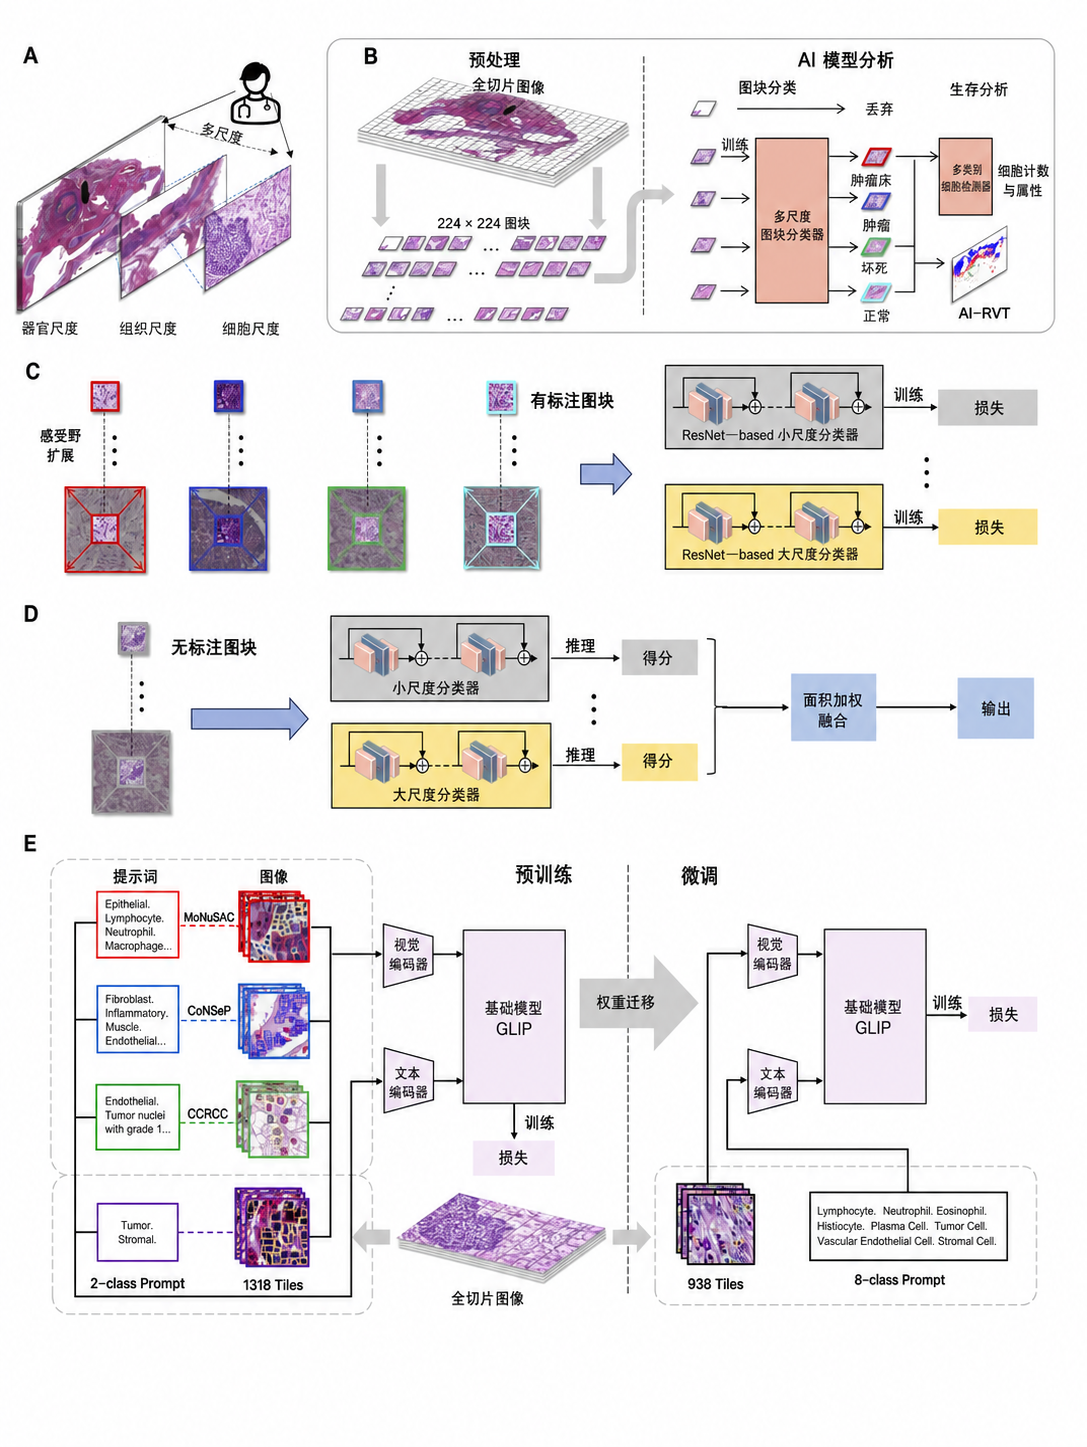
\includegraphics[width=0.88\textwidth,height=0.58\textheight,keepaspectratio]{figures/lung_image8_zh.png}
  \caption{多尺度 WSI 分析与细胞检测流程}
  \label{fig:lung_pipeline}
\end{figure}
图~\ref{fig:lung_pipeline} 将本章的两条技术路径置于同一分析框架中。（A--D）对应区域级分析：首先模拟病理医师由低倍到高倍的阅片过程，再把超大尺寸 WSI 切分为空间对齐的多尺度图块；不同尺度分类器分别判断活性肿瘤、肿瘤床、坏死和正常组织，最终依据各类区域的面积占比完成切片级与患者级 AI-RVT 计算。该流程强调局部细胞形态必须结合较大范围的组织结构进行解释，因而能够减少单尺度图块在肿瘤--间质交界处产生的类别混淆。\par 图中（E）对应细胞级分析。GLIP 检测器依次经历公共多类细胞核数据预训练、目标域肿瘤/间质粗粒度适配以及八类细胞精细标注训练，使通用视觉语言表征逐步适应肺鳞癌 H\&E 图像。两条路径在输出层面形成互补：区域分支给出残余肿瘤负荷，细胞分支提供肿瘤周围免疫和间质细胞的类别与坐标，二者共同构成后续生存分析所需的可解释变量。数据集名称、类别提示词和模型名称作为实际训练输入保留英文。

\section{实验设置}
本节只说明数据来源、标注与预处理、模型训练参数以及临床统计口径；算法设计动机和公式已在上一节给出，所有性能数值、对照表和显著性检验结果统一置于“实验结果与分析”，避免设置与结论交叉。

\subsection{数据集准备}
研究数据来自国家癌症中心（National Cancer Center, NCC）、山西省肿瘤医院（Shanxi Cancer Hospital, SXCH）和深圳市肿瘤医院（Shenzhen Cancer Hospital, SZCH），总体设计如图 \ref{fig:lung_study_design} 所示。

训练数据队列 NCC\_Cohort1 包含 20 例患者的 251 张病理医师精细标注 WSI，用于训练多尺度区域分类器和构建域内细胞检测数据。外部验证数据队列 SXCH 包含 28 例患者的 192 张 WSI，用于评价 AI-RVT 与病理医师视觉评估结果 VIS-RVT 在切片级和患者级的一致性。独立测试数据由 NCC\_Cohort2 的 51 例患者和 SZCH 的 32 例患者构成；在预后分析中进一步合并 NCC\_Cohort1 的 20 例患者，最终形成 103 例患者的生存队列。该队列中 78 例为 non-pCR 患者，占 75.7\%，是术后风险分层的重点对象。具有完整患者级 VIS-RVT 和 AI-RVT 的 84 例患者被纳入 MPR 一致性分析。
数据集预处理细节：医生使用openslide工具手动在WSI图片文件上进行标注，由于一般的WSI图都十分庞大，长宽一般为数十万像素到上百万像素尺度，进行大范围内的逐个的实例级标注是不现实的，过于耗费人力和时间。实验医生只进行两种标注任务：1.以整张WSI的缩略图为依据，在整张WSI图内画圈方式圈出多个区域，然后标明每个区域具体的区域类型（比如瘤床区，坏死区，肿瘤区） 2.对采样出的大量小范围的病理切片区域，进行细致的逐实例标注。标注任务2与前一个标注任务相比，更要求细致、精准、无遗漏，而不苛求过大的实例量。前期实验中发现对于标注任务2以及基于它的细胞检测模型训练，只需要每类数百甚至数十个实例就足以取得比较满意的最终检测效果。

\subsection{标注任务与数据预处理}
由于一般的 WSI 图像十分庞大，长宽通常达到数十万像素甚至上百万像素尺度，在整张切片上逐个完成实例级标注并不现实，会消耗大量人力和时间。因此，实验医生通常需要区分两类标注任务。第一类是在整张 WSI 的缩略图上，以闭合曲线或多边形圈出若干区域，并为每个区域指定区域类型，例如肿瘤床区、坏死区或活性肿瘤区。第二类是对采样得到的大量小范围病理图块进行细致的逐实例标注，为每一个可辨认的细胞或细胞核勾画独立轮廓。与区域级标注相比，第二类任务要求更细致、精准并尽量避免遗漏，但不以覆盖尽可能多的实例为目标。前期实验表明，对于逐实例标注及基于这些标注训练的细胞检测模型，每一类只需要数百个甚至数十个质量可靠的实例，通常就能够取得较为稳定的最终检测效果。

两类标注的差异会直接影响检测模型所接收的监督信号。图 \ref{fig:annotation_task_comparison} 给出了同一类病理图块的对照示例，其中裁剪区域内的绿色实例来自 GeoJSON 标注中的“淋巴细胞（Lymphocyte）”类别。A 中这些细胞虽然在图像中客观存在，但没有全部被逐一勾画；B 则对相应细胞补充了独立的实例轮廓。对于采用实例检测或实例分割损失的训练流程，如果未标注区域被直接编码为背景或参与负样本匹配，A 中未被勾画的淋巴细胞就可能被模型当作背景，从而同时产生漏检倾向和前景--背景监督冲突。A 表示监督信息不完整，其中未勾画的淋巴细胞会被错误编码为负样本；B 通过完整实例轮廓提供更明确的“一个细胞对应一个实例”的正向约束。因此，本研究在构建细胞检测训练集时优先使用小图块中的高质量逐实例标注，并将区域级标注主要用于 WSI 组织区域分类和多尺度上下文建模。

\begin{figure}[tb]
  \centering
  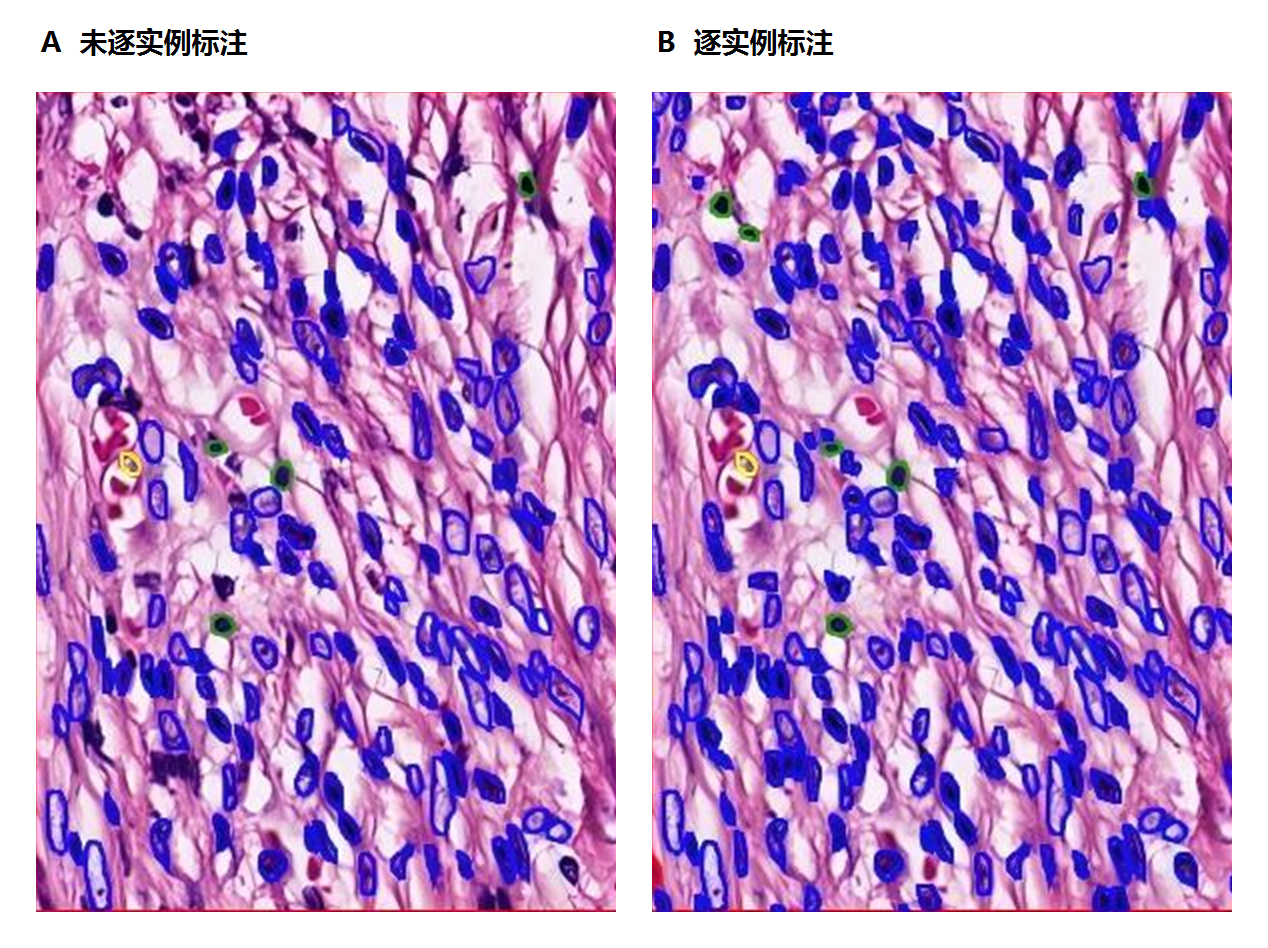
\includegraphics[width=0.76\textwidth]{figures/annotation_task_comparison_recrop_20260824.png}
  \caption{两种实例标注完整性对比}
  \label{fig:annotation_task_comparison}
\end{figure}
图~\ref{fig:annotation_task_comparison} 中，A 表示未完成逐实例标注的版本，B 表示完成逐实例标注的版本；绿色轮廓标出淋巴细胞实例。A 中可见细胞未被全部转化为独立实例轮廓，若训练流程将未标注区域作为背景处理，可能造成前景细胞与背景标签之间的监督冲突；B 为细胞检测模型提供了更完整的实例级正样本。

\subsubsection{WSI 图块生成与染色归一化}
原始 WSI 统一重采样至 20 倍放大倍率，对应约 $0.5\,\mu\mathrm{m}/\mathrm{pixel}$。病理医师以闭合多边形标注肿瘤床、活性肿瘤、坏死和正常区域，程序将 WSI 划分为互不重叠的 $224\times224$ 像素图块。每个图块先转换为灰度图；若亮度范围低于完整动态范围的 35\%，则判定其主要为空白并剔除。对于其余图块，计算四类病理区域的面积占比，仅当某一类别覆盖超过 60\% 时才赋予相应标签，否则舍弃，以减少边界混合图块引入的监督噪声。该流程共获得 975,359 个训练图块。

跨中心染色差异采用 Vahadane 方法进行归一化。该方法借助非负矩阵分解将图像表示为染色浓度矩阵与颜色基矩阵，再把目标切片的颜色基对齐至参考切片并重建图像。与简单颜色直方图匹配相比，这一过程更有利于保留细胞核和间质纹理，同时降低不同中心制片流程造成的颜色偏移。

\subsection{多尺度区域分类配置}
原始 WSI 统一重采样到 20 倍放大倍率（约 $0.5\,\mu\mathrm{m}/\mathrm{pixel}$），以 $224\times224$ 像素为基本图块。病理区域覆盖率超过 60\% 时才赋予类别标签，亮度动态范围不足 35\% 的空白图块予以剔除。多尺度分类器均采用 ResNet-101，优化器为 SGD，基础学习率为 $10^{-4}$，批大小为 4，损失函数为带类别权重的多类别交叉熵。类别权重用于增加稀少活性肿瘤图块在训练中的贡献。为保证尺度消融只反映感受野差异，各尺度使用一致的患者级划分、中心坐标、染色归一化和训练轮次；多尺度结果先在图块级独立输出，再按组织面积完成切片级融合。

\subsection{渐进式细胞检测配置}
细胞检测以 GLIP-L 为视觉语言骨架，保持“公开病理预训练--目标域粗粒度适配--目标域细粒度精调”的三阶段顺序。过程一使用 MoNuSAC、CCRCC 和 CoNSeP 等公开数据，并先统一不同数据集的细胞语义名称；过程二从 NCC\_Cohort1 的 7 例患者中提取 1,318 个图块，以 Tumor/Stromal 粗粒度标签完成染色和组织背景适配；过程三从完整逐实例标注区域重叠采样 938 个 $224\times224$ 图块，训练 Tumor cell、Lymphocyte、Neutrophil、Eosinophil、Plasma Cell、Endothelial Cell、Fibroblast 和 Histiocyte 八类细胞。另按相同预处理策略固定 8 个测试图块用于检测评价。与渐进式模型比较的通用 GLIP 和 Mask R-CNN 对照使用相同目标域训练/测试划分，避免数据量差异成为混杂因素。

\subsection{临床评价指标与统计分析}
本章使用的肺鳞癌数字病理数据与前几章的 patch 级核检测分割数据不同。该工作更接近临床队列研究，并以患者、切片或全切片图像为分析单位，重点评估 AI 量化指标与病理缓解程度、免疫细胞密度、无病生存和总生存之间的关系。因此，该章实验需要同时考虑图像处理流程和临床统计流程。

这类数据的特殊性在于，模型输出构成临床指标计算的中间表征层，并进一步汇总为患者级定量指标。例如，残余可存活肿瘤比例需要由组织区域识别结果推导，肿瘤周围免疫细胞密度需要由细胞检测结果和空间边界关系共同决定。相比检测或分割 benchmark，这类研究更加重视量化指标的可解释性、稳定性和临床相关性。

第五章采用独立的 Lung-AI 图像资源，正文已分别说明研究队列、区域分类、AI-RVT 与 VIS-RVT 一致性、连续 RVT 风险分析以及肿瘤周围免疫细胞联合分层。该实验的可复现性依赖三个关键环节：第一，训练、验证和预后测试患者必须按原研究设计隔离；第二，RVT 需要先在切片级进行面积加权，再聚合到患者级；第三，免疫细胞密度必须记录相对于肿瘤边界的距离范围，确保 $50\,\mu\mathrm{m}$ 和 $700\,\mu\mathrm{m}$ 的统计量具有一致定义。

本章涉及的临床统计指标包括组间差异、相关性分析、ICC 一致性、风险比以及生存曲线等。这些统计分析用于检验 AI 量化指标与病理评估和患者结局之间的稳定关系。对于这类实验，模型性能的最终价值体现在能否形成可解释的临床分层，而不是单纯在图像层面取得高分。

研究以 DFS 和 OS 为临床终点。RVT 同时以两种方式进入分析：一是采用 10\% 阈值区分 MPR 与 non-MPR，二是保留连续比例，以减少阈值二分造成的信息损失。组间生存差异采用 Kaplan--Meier 曲线和 log-rank 检验；DFS 使用标准 Cox 比例风险模型；由于 OS 事件数较少，OS 多变量分析采用 Firth 惩罚 Cox 回归，以降低小样本偏倚并提高风险比估计的稳定性。所有患者级 RVT 均由该患者全部可用切片的 RVT 百分比取算术平均得到。

\section{实验结果与分析}
\subsection{标注完整性实验}
为了定量说明逐实例标注完整性对模型评价的影响，本研究进一步整理同一肺部病理验证任务的两批实验结果。图中 A 表示未完成逐实例补充的标注状态，B 表示经过补充、实例覆盖更完整的标注状态。这里的 A/B 是对标注版本的区分，采用的模型是一致的，都是GLIP-L带有分割头和检测头的标准版本。

表~\ref{tab:annotation_ab_full_metrics} 汇总了两批结果的主要指标。与 A 相比，B 的 Dice、AJI、Diceobj、PQ、F1 和 mAP 均更高。也就是说，在这组实际历史评测中，补充逐实例标注后，模型输出与金标准之间的实例匹配和整体检测统计更加充分；若只观察单一像素级指标，则可能低估标注完整性带来的影响。

\begin{table}[htbp]
  \centering
  \caption{标注完整性对总体性能的影响}
  \label{tab:annotation_ab_full_metrics}
  \resizebox{\textwidth}{!}{%
  \begin{tabular}{llrrrrrrr}
    \toprule
    版本 & 标注含义 & 图块数 & Dice & AJI & Diceobj & PQ & F1 & mAP \\
    \midrule
    A & 未完成逐实例补充 & 8 & 0.709 & 0.433 & 0.710 & 0.328 & 0.668 & 0.2884 \\
    B & 补充完整逐实例标注 & 8 & 0.766 & 0.450 & 0.750 & 0.350 & 0.748 & 0.3750 \\
    \bottomrule
  \end{tabular}}
\end{table}

为了更直观地呈现差异，表~\ref{tab:annotation_ab_delta} 进一步给出了 B 相对于 A 的绝对变化量和相对变化率。B 的 Dice 提高了 0.057，Diceobj 提高了 0.040，AJI 提高了 0.017，PQ 提高了 0.022，F1 提高了 0.080，mAP 提高了 0.0866；其中 mAP 的相对提升达到约 30.0\%，F1 的相对提升约为 12.0\%。这些变化说明，遗漏的细胞实例不仅会减少监督信息，还会改变预测结果与真实实例之间的匹配关系，使评价结果对细胞的检出能力和实例对应关系更加敏感。

\begin{table}[htbp]
  \centering
  \caption{补全实例标注前后的指标变化}
  \label{tab:annotation_ab_delta}
  \begin{tabular}{lrrrr}
    \toprule
    指标 & A & B & 绝对变化（B-A） & 相对变化 \\
    \midrule
    Dice & 0.709 & 0.766 & +0.0570 & +8.0\% \\

    AJI & 0.433 & 0.450 & +0.0170 & +3.9\% \\
    Diceobj & 0.710 & 0.750 & +0.0400 & +5.6\% \\
    PQ & 0.328 & 0.350 & +0.0220 & +6.7\% \\
    F1 & 0.668 & 0.748 & +0.0800 & +12.0\% \\
    mAP & 0.2884 & 0.3750 & +0.0866 & +30.0\% \\
    \bottomrule
  \end{tabular}
\end{table}

上述结果与前文的机制分析相互印证：在 A 中，图像中客观存在但没有被逐一勾画的淋巴细胞可能在训练或评价过程中被当作背景，因而造成前景与背景监督信号混杂；在 B 中，相应淋巴细胞被补充为独立实例，模型输出与金标准之间的实例级对应关系得到更完整的统计。本文将表~\ref{tab:annotation_ab_full_metrics} 和表~\ref{tab:annotation_ab_delta} 作为标注完整性影响的实验证据和支持性分析，不将其夸大为严格控制所有模型权重变量的因果实验。它至少表明：在相同验证数据规模和评价口径下，标注版本的完整程度足以带来明显的性能差异；因此，后续模型训练应优先采用高质量、少遗漏的逐实例标注，并将区域级标注与实例级标注严格区分。

\subsection{区域分类与细胞检测性能}
图~\ref{fig:lung_region_performance}（a）显示，多尺度模型在肿瘤床、活性肿瘤、坏死和正常组织四类区域上均优于单尺度模型。六次独立实验中，平均 F1 从 $0.532\pm0.005$ 提升至 $0.784\pm0.002$，平均精确率从 $0.584\pm0.003$ 提升至 $0.866\pm0.003$，平均召回率从 $0.486\pm0.003$ 提升至 $0.746\pm0.005$；三项指标的相对提升分别为 47.2\%、48.2\% 和 53.3\%。坏死区域的 F1 从 0.426 提高到 0.792，说明大尺度组织上下文对治疗后结构判定尤为重要。

多类细胞检测以相同训练流程下的 Mask R-CNN 和未经额外病理预训练的 GLIP 为对照。渐进式训练模型在七类非肿瘤细胞上的平均 AP50 为 $66.14\pm0.58$，高于 GLIP 对照的 $53.07\pm2.60$ 和 Mask R-CNN 的 $32.26\pm1.40$。其中浆细胞 AP50 达到 $73.57\pm3.18$，相较 GLIP 对照的 $29.33\pm3.10$ 提升明显；这说明公共病理数据预训练和域内粗粒度适配能够缓解小样本细胞类别的过拟合。

\begin{table}[htbp]
  \centering
  \caption{区域分类与细胞检测总体性能}
  \label{tab:lung_model_performance}
  \resizebox{0.98\textwidth}{!}{%
  \begin{tabular}{llll}
    \toprule
    任务 & 方法 & 指标 & 结果（均值$\pm$标准差） \\
    \midrule
    区域分类 & 单尺度 & 平均 F1 / Precision / Recall & $0.532\pm0.005$ / $0.584\pm0.003$ / $0.486\pm0.003$ \\
    区域分类 & 多尺度 & 平均 F1 / Precision / Recall & $0.784\pm0.002$ / $0.866\pm0.003$ / $0.746\pm0.005$ \\
    细胞检测 & Mask R-CNN & 七类平均 AP50 & $32.26\pm1.40$ \\
    细胞检测 & GLIP（无额外预训练） & 七类平均 AP50 & $53.07\pm2.60$ \\
    细胞检测 & 渐进式训练模型 & 七类平均 AP50 & $66.14\pm0.58$ \\
    \bottomrule
  \end{tabular}}
\end{table}

\begin{figure}[tb]
  \centering
  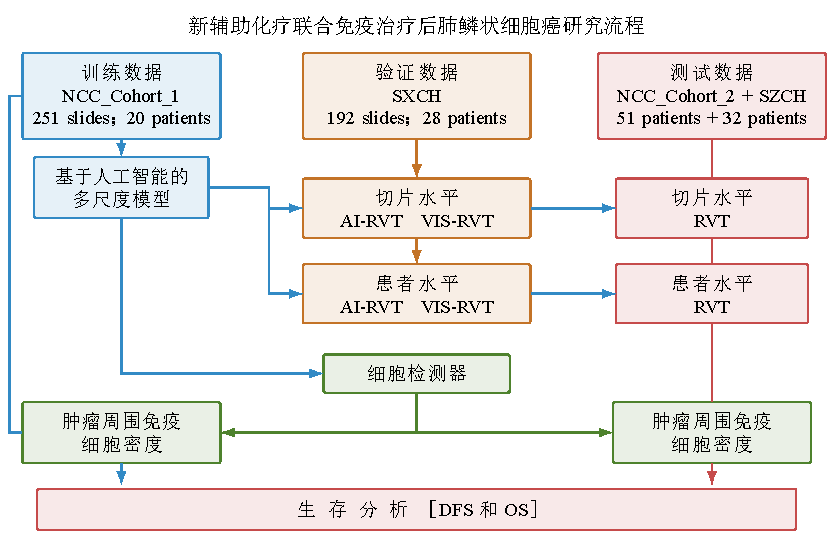
\includegraphics[width=0.92\textwidth]{chapters/lung_study_design_compact.pdf}
  \caption{多中心研究设计}
  \label{fig:lung_study_design}
\end{figure}
图~\ref{fig:lung_study_design} 中，NCC\_Cohort1 用于模型训练，SXCH 用于外部一致性验证，NCC\_Cohort2 与 SZCH 构成独立测试数据；预后分析进一步联合 NCC\_Cohort1。


\begin{table}[htbp]
  \centering
  \caption{多中心队列构成}
  \label{tab:lung_cohorts}
  \resizebox{0.98\textwidth}{!}{%
  \begin{tabular}{llll}
    \toprule
    阶段 & 队列 & 数据规模 & 主要用途 \\
    \midrule
    模型训练 & NCC\_Cohort1 & 20 例，251 张 WSI & 多尺度区域分类与域内细胞建模 \\
    外部验证 & SXCH & 28 例，192 张 WSI & 切片级、患者级 RVT 一致性 \\
    独立测试 & NCC\_Cohort2、SZCH & 51 例、32 例 & 独立测试与空间免疫分析 \\
    预后分析 & NCC\_Cohort1/2、SZCH & 103 例，其中 non-pCR 78 例 & DFS、OS 及联合风险分层 \\
    细胞精调 & NCC\_Cohort1 标注区 & 938 个 $224\times224$ 图块 & 八类细胞检测与分类 \\
    \bottomrule
  \end{tabular}}
\end{table}

\subsection{渐进式训练消融}
\begin{table}[htbp]
  \centering
  \caption{多类细胞检测渐进式训练结果}
  \label{tab:lung_stage_training}
  \resizebox{0.98\textwidth}{!}{%
  \begin{tabular}{p{0.14\textwidth}p{0.26\textwidth}p{0.29\textwidth}p{0.25\textwidth}}
    \toprule
    阶段或对照 & 训练数据与初始化 & 主要作用 & 结果表现 \\
    \midrule
    过程一：公开病理预训练
    & MoNuSAC、CCRCC、CoNSeP；以 GLIP-L 预训练参数初始化
    & 学习跨公开病理数据集的细胞形态、纹理和视觉--语言类别对应关系
    & 为目标域适配提供公开医学视觉先验 \\
    过程二：目标域粗粒度适配
    & NCC\_Cohort1 的 1,318 个图块；Tumor 和 Stromal 两类标签
    & 适应本研究队列的染色、组织背景和肿瘤--间质结构，减少细粒度噪声
    & 为细粒度细胞精调提供目标域初始化 \\
    过程三：目标域细粒度精调
    & 938 个 $224\times224$ 图块；八类细胞逐实例标注
    & 学习细胞类别、实例边界和密集场景下的区域匹配
    & 作为后续定量比较的最佳渐进式训练结果 \\
    无公开医学预训练对照
    & 以通用 GLIP 参数初始化，在目标域训练集上训练，并在验证集上测试
    & 去除公开医学数据预训练，测量通用 GLIP 直接适配病理数据的能力
    & GLIP 对照七类平均 AP50 为 $53.07\pm2.60$ \\
    Mask R-CNN 对照
    & 使用相同目标域数据流程，但不使用视觉--语言预训练
    & 检验性能提升是否来自渐进式视觉语言适配，而非单纯检测头
    & 七类平均 AP50 为 $32.26\pm1.40$ \\
    \bottomrule
  \end{tabular}}
\end{table}


三阶段训练的效果由表~\ref{tab:lung_model_performance} 中的对照结果进一步体现。未经额外公开医学病理数据预训练的 GLIP 在七类非肿瘤细胞上的平均 AP50 为 $53.07\pm2.60$，而采用渐进式公开病理预训练、目标域粗粒度适配和细粒度精调后的模型达到 $66.14\pm0.58$，绝对提高 $13.07$ 个百分点，相对提升约 $24.6\%$。在相同任务下，Mask R-CNN 的七类平均 AP50 为 $32.26\pm1.40$，明显低于两种 GLIP 配置。尤其对于浆细胞等训练样本较少的类别，渐进式训练模型的 AP50 达到 $73.57\pm3.18$，而未额外预训练的 GLIP 对照仅为 $29.33\pm3.10$。这说明公开医学数据预训练首先提供了可迁移的细胞视觉语义，目标域粗粒度适配随后修正染色和组织背景差异，最后的高质量逐实例精调才将这些先验转化为目标队列中的细粒度检测能力。

因此，过程一并不是可有可无的预热步骤，而是整个训练链路中负责建立医学视觉先验的基础环节。若直接从通用 GLIP 权重进入目标域细粒度训练，模型需要在有限的目标域实例上同时学习病理外观、类别语义和实例定位，容易造成小类别过拟合和跨类别混淆。表中的 GLIP 对照与渐进式模型之间的差异，正是对这一训练策略必要性的定量验证。

\subsection{基线临床病理特征}
我们按照中心汇总了 71 例 NCC 患者（NCC\_Cohort1 与 NCC\_Cohort2）、28 例 SXCH 患者和 32 例 SZCH 患者的基线特征，见表 \ref{tab:lung_baseline}。三中心在性别、VIS-RVT、ypT、ypN 和 MPR 分布方面总体可比，年龄分布存在统计学差异（$p=0.031$）。因此，后续生存模型除考察 RVT 和空间免疫指标外，还将治疗后淋巴结状态 ypN 纳入校正。

\begin{table}[htbp]
  \centering
  \caption{患者基线临床病理特征}
  \label{tab:lung_baseline}
  \resizebox{\textwidth}{!}{%
  \begin{tabular}{lcccc}
    \toprule
    特征 & NCC（$N=71$） & SXCH（$N=28$） & SZCH（$N=32$） & $p$ 值 \\
    \midrule
    男性，$n$（\%） & 70（99\%） & 28（100\%） & 29（91\%） & 0.092 \\
    年龄，中位数（Q1，Q3） & 60.00（55.00，65.00） & 63.50（60.50，66.00） & 64.50（59.50，68.50） & 0.031 \\
    VIS-RVT，中位数（Q1，Q3） & 0.03（0.00，0.38） & 0.00（0.00，0.10） & 0.01（0.00，0.13） & 0.300 \\
    \midrule
    ypT 分期 & & & & 0.140 \\
    \quad T0 & 26（37\%） & 13（46\%） & 8（25\%） & \\
    \quad Tis & 1（1.4\%） & 0（0\%） & 0（0\%） & \\
    \quad T1 & 25（35\%） & 11（39\%） & 20（63\%） & \\
    \quad T2 & 13（18\%） & 3（11\%） & 3（9.4\%） & \\
    \quad T3 & 6（8.5\%） & 1（3.6\%） & 0（0\%） & \\
    \quad T4 & 0（0\%） & 0（0\%） & 1（3.1\%） & \\
    \midrule
    ypN 分期 & & & & 0.110 \\
    \quad N0 & 37（52\%） & 23（82\%） & 20（63\%） & \\
    \quad N1 & 19（27\%） & 3（11\%） & 7（22\%） & \\
    \quad N2 & 15（21\%） & 2（7.1\%） & 5（16\%） & \\
    \midrule
    病理缓解 & & & & 0.300 \\
    \quad MPR & 42（59\%） & 21（75\%） & 22（69\%） & \\
    \quad non-MPR & 29（41\%） & 7（25\%） & 10（31\%） & \\
    \bottomrule
  \end{tabular}}
  \vspace{0.3em}

  \raggedright 注：分类变量以 $n$（\%）表示，连续变量以中位数（Q1，Q3）表示；根据变量类型采用 Fisher 精确检验、Kruskal--Wallis 秩和检验或 Pearson 卡方检验。
\end{table}

\subsection{多尺度区域与多类细胞检测结果}
\begin{table}[htbp]
  \centering
  \caption{感受野消融结果}
  \label{tab:lung_receptive_field_ablation}
  \resizebox{\textwidth}{!}{%
  \begin{tabular}{llllll}
    \toprule
    设置 & 感受野/尺度 & 融合策略 & F1（\%）$\uparrow$ & 精确度（\%）$\uparrow$ & 召回率（\%）$\uparrow$ \\
    \midrule
    感受野不足（单尺度/小上下文） & $224\times224$ pixel & 无多尺度融合 & 53.2$\pm$0.5 & 58.4$\pm$0.3 & 48.6$\pm$0.3 \\
    感受野充分（多尺度/大上下文） & $672\times672$ pixel & 多尺度融合 & 78.4$\pm$0.2 & 86.6$\pm$0.3 & 74.6$\pm$0.5 \\
    \bottomrule
  \end{tabular}%
  }
\end{table}



表~\ref{tab:lung_receptive_field_ablation} 比较了单尺度小上下文与多尺度大上下文两种区域分类设置。单尺度模型的平均 F1、精确度和召回率分别为 53.2\% 、58.4\% 和 48.6\%；引入多尺度上下文与融合策略后，三项指标分别提升至 78.4\% 、86.6\% 和 74.6\%。相对于单尺度设置，F1、精确度和召回率的相对提升分别为 47.2\%、48.2\% 和 53.3\%。这表明，单个局部图块提供的组织上下文不足以稳定区分肿瘤床、活性肿瘤、坏死和正常组织，而扩大感受野并进行尺度融合能够利用更完整的组织结构信息，从而同时改善分类的正确性与覆盖能力。

\begin{figure}[tb]
  \centering
  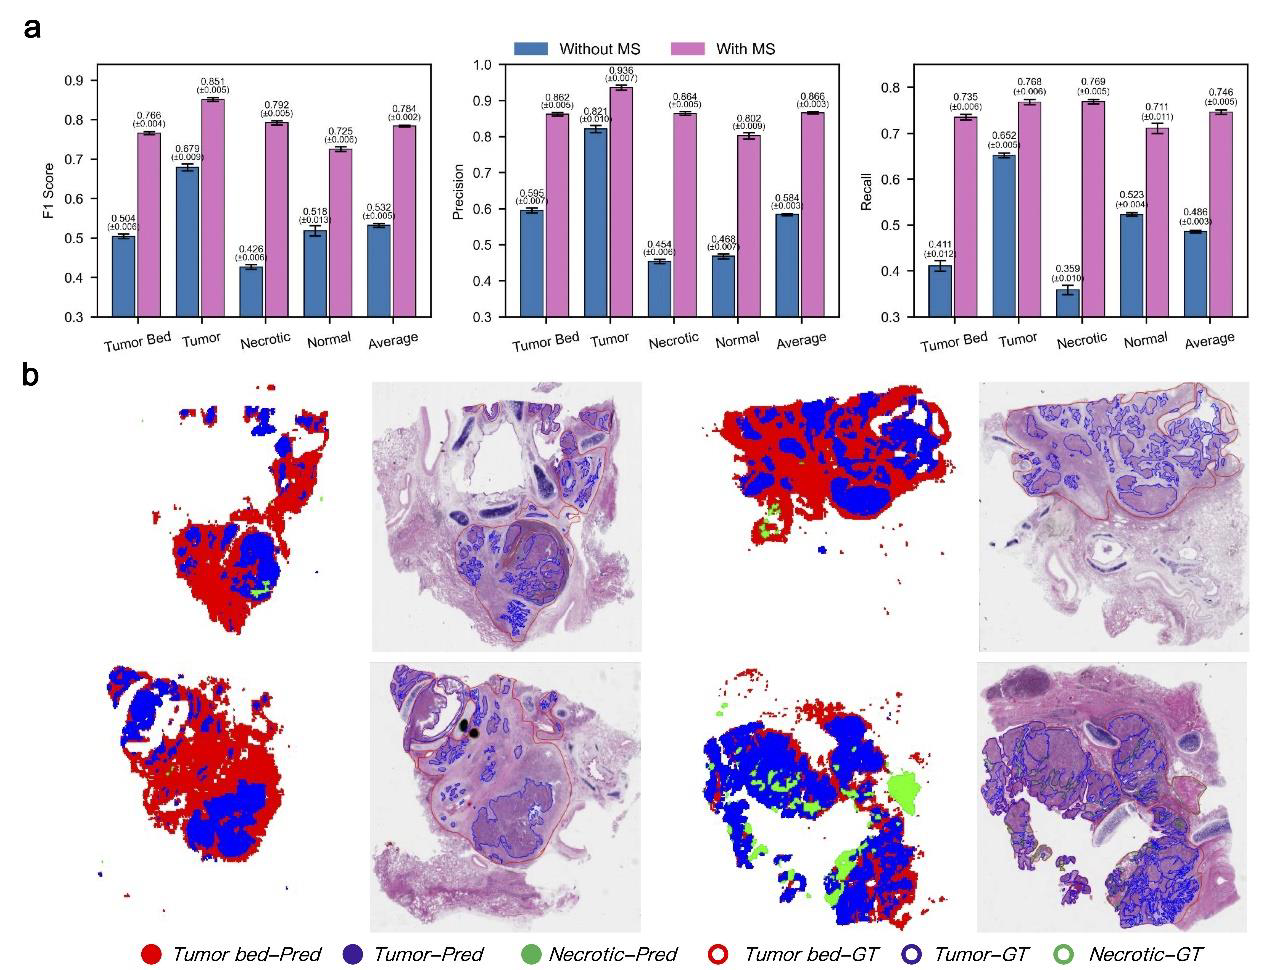
\includegraphics[width=0.76\textwidth]{chapters/lung_fig5_4_ab_20260824.png}
  \caption{多尺度区域分类性能与 WSI 级空间对照}
  \label{fig:lung_region_performance}
\end{figure}
图~\ref{fig:lung_region_performance} 专门考察区域级分析。（a）比较单尺度与多尺度模型在肿瘤床、活性肿瘤、坏死和正常组织四类区域上的 F1、精确率与召回率。引入多尺度上下文后，平均 F1 由 $0.532\pm0.005$ 提升至 $0.784\pm0.002$，平均精确率由 $0.584\pm0.003$ 提升至 $0.866\pm0.003$，平均召回率由 $0.486\pm0.003$ 提升至 $0.746\pm0.005$。其中坏死区域的 F1 从 0.426 提高到 0.792，表明治疗后坏死与间质的区分尤其依赖较大范围组织结构。（b）给出 WSI 级预测与病理标注的空间对照，大面积主体区域总体一致，差异主要集中在活性肿瘤、坏死与治疗后间质交织的边界。该结果说明多尺度模型不仅提高了总体统计量，也使区域面积量化更符合病理阅片中的空间连续性。

\begin{figure}[tb]
  \centering
  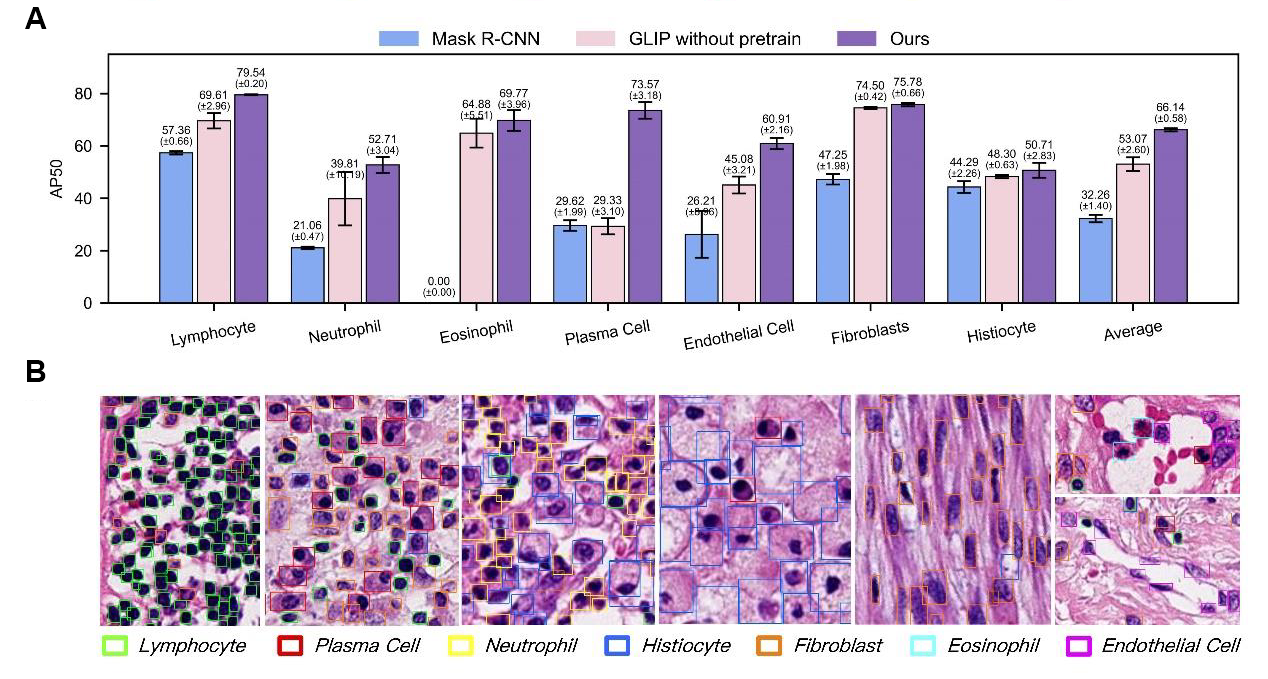
\includegraphics[width=0.84\textwidth]{chapters/lung_fig5_4_cd_precise_ab_20260829.png}
  \caption{多类细胞检测性能与代表性结果}
  \label{fig:lung_cell_performance}
\end{figure}
图~\ref{fig:lung_cell_performance} 转向细胞级分析。（A）比较 Mask R-CNN、未经额外医学预训练的 GLIP 与渐进式训练模型在七类肿瘤周围细胞上的 AP50。渐进式训练模型的七类平均 AP50 为 $66.14\pm0.58$，高于 GLIP 对照的 $53.07\pm2.60$ 和 Mask R-CNN 的 $32.26\pm1.40$；浆细胞等小样本类别的提升尤为明显，验证了公开病理预训练、目标域粗粒度适配和细粒度精调的递进作用。（B）展示多个代表性图块中的分类与定位结果。模型能够在密集、形态相似且染色变化明显的区域同时输出细胞类别和位置，为后续以肿瘤边界为参照的径向密度计算提供实例基础。

\subsection{肺癌细胞联合检测与实例分割结果}
为补充前述细胞检测实验，本研究在原有肺癌数据处理流程上启用原生实例分割头，并固定训练至 4000 次迭代后导出最终模型。评价集包含 8 个 $224\times224$ 病理图块和 669 个逐实例标注。评价标注保留了 9 个历史类别编号，其中嗜酸性粒细胞及其细胞核分别记录为两个标签；因此，本节的目的主要是验证同一视觉语言骨架能否同时输出可用的检测框与非矩形实例掩膜，而不是据此替代患者级临床验证。

表~\ref{tab:lung_native_segmentation_final4000} 给出固定 4000 次迭代模型的最终结果。独立使用 COCO API 复算后，检测任务的 AP、AP50 和 AP75 分别为 0.315、0.604 和 0.278，分割任务的对应指标分别为 0.242、0.514 和 0.175。在置信度阈值固定为 0.5 时，将各类别实例掩膜合并为前景区域后，8 个图块的前景 Dice 宏平均为 0.779，像素汇总 Dice 为 0.773。最终文件共包含 831 个可解码实例掩膜，8 个图块均有检测与分割输出，未发现空掩膜；其中 7 个掩膜的离散轮廓恰好呈矩形，占全部输出的 0.84\%，说明绝大多数输出确实具有实例边界形状，但少量紧凑目标仍可能退化为近似框形轮廓。

\begin{table}[htbp]
  \centering
  \caption{肺癌细胞检测与实例分割的固定终点评价结果}
  \label{tab:lung_native_segmentation_final4000}
  \resizebox{\textwidth}{!}{%
  \begin{tabular}{lcccccccc}
    \toprule
    设置 & BBox AP & BBox AP50 & BBox AP75 & BBox AR100 & Segm AP & Segm AP50 & Segm AP75 & Segm AR100 \\
    \midrule
    历史检测基线 & 0.065 & 0.137 & 0.053 & 0.251 & -- & -- & -- & -- \\
    原生检测--分割模型（4000 次迭代） & 0.315 & 0.604 & 0.278 & 0.461 & 0.242 & 0.514 & 0.175 & 0.327 \\
    \bottomrule
  \end{tabular}}
\end{table}

历史检测基线仅输出边界框，不包含可比较的实例掩膜；其与最终模型之间的训练初始化和监督目标也并非完全相同。因此，表~\ref{tab:lung_native_segmentation_final4000} 中检测指标的差异只能作为流程级描述性对照，不能单独归因于“增加分割头”。可以确认的是，最终联合模型在同一批测试图块上同时给出了有效的检测与分割结果，从而补足了仅依赖框级定位时无法量化细胞轮廓、面积和接触边界的不足。

\begin{figure}[tb]
  \centering
  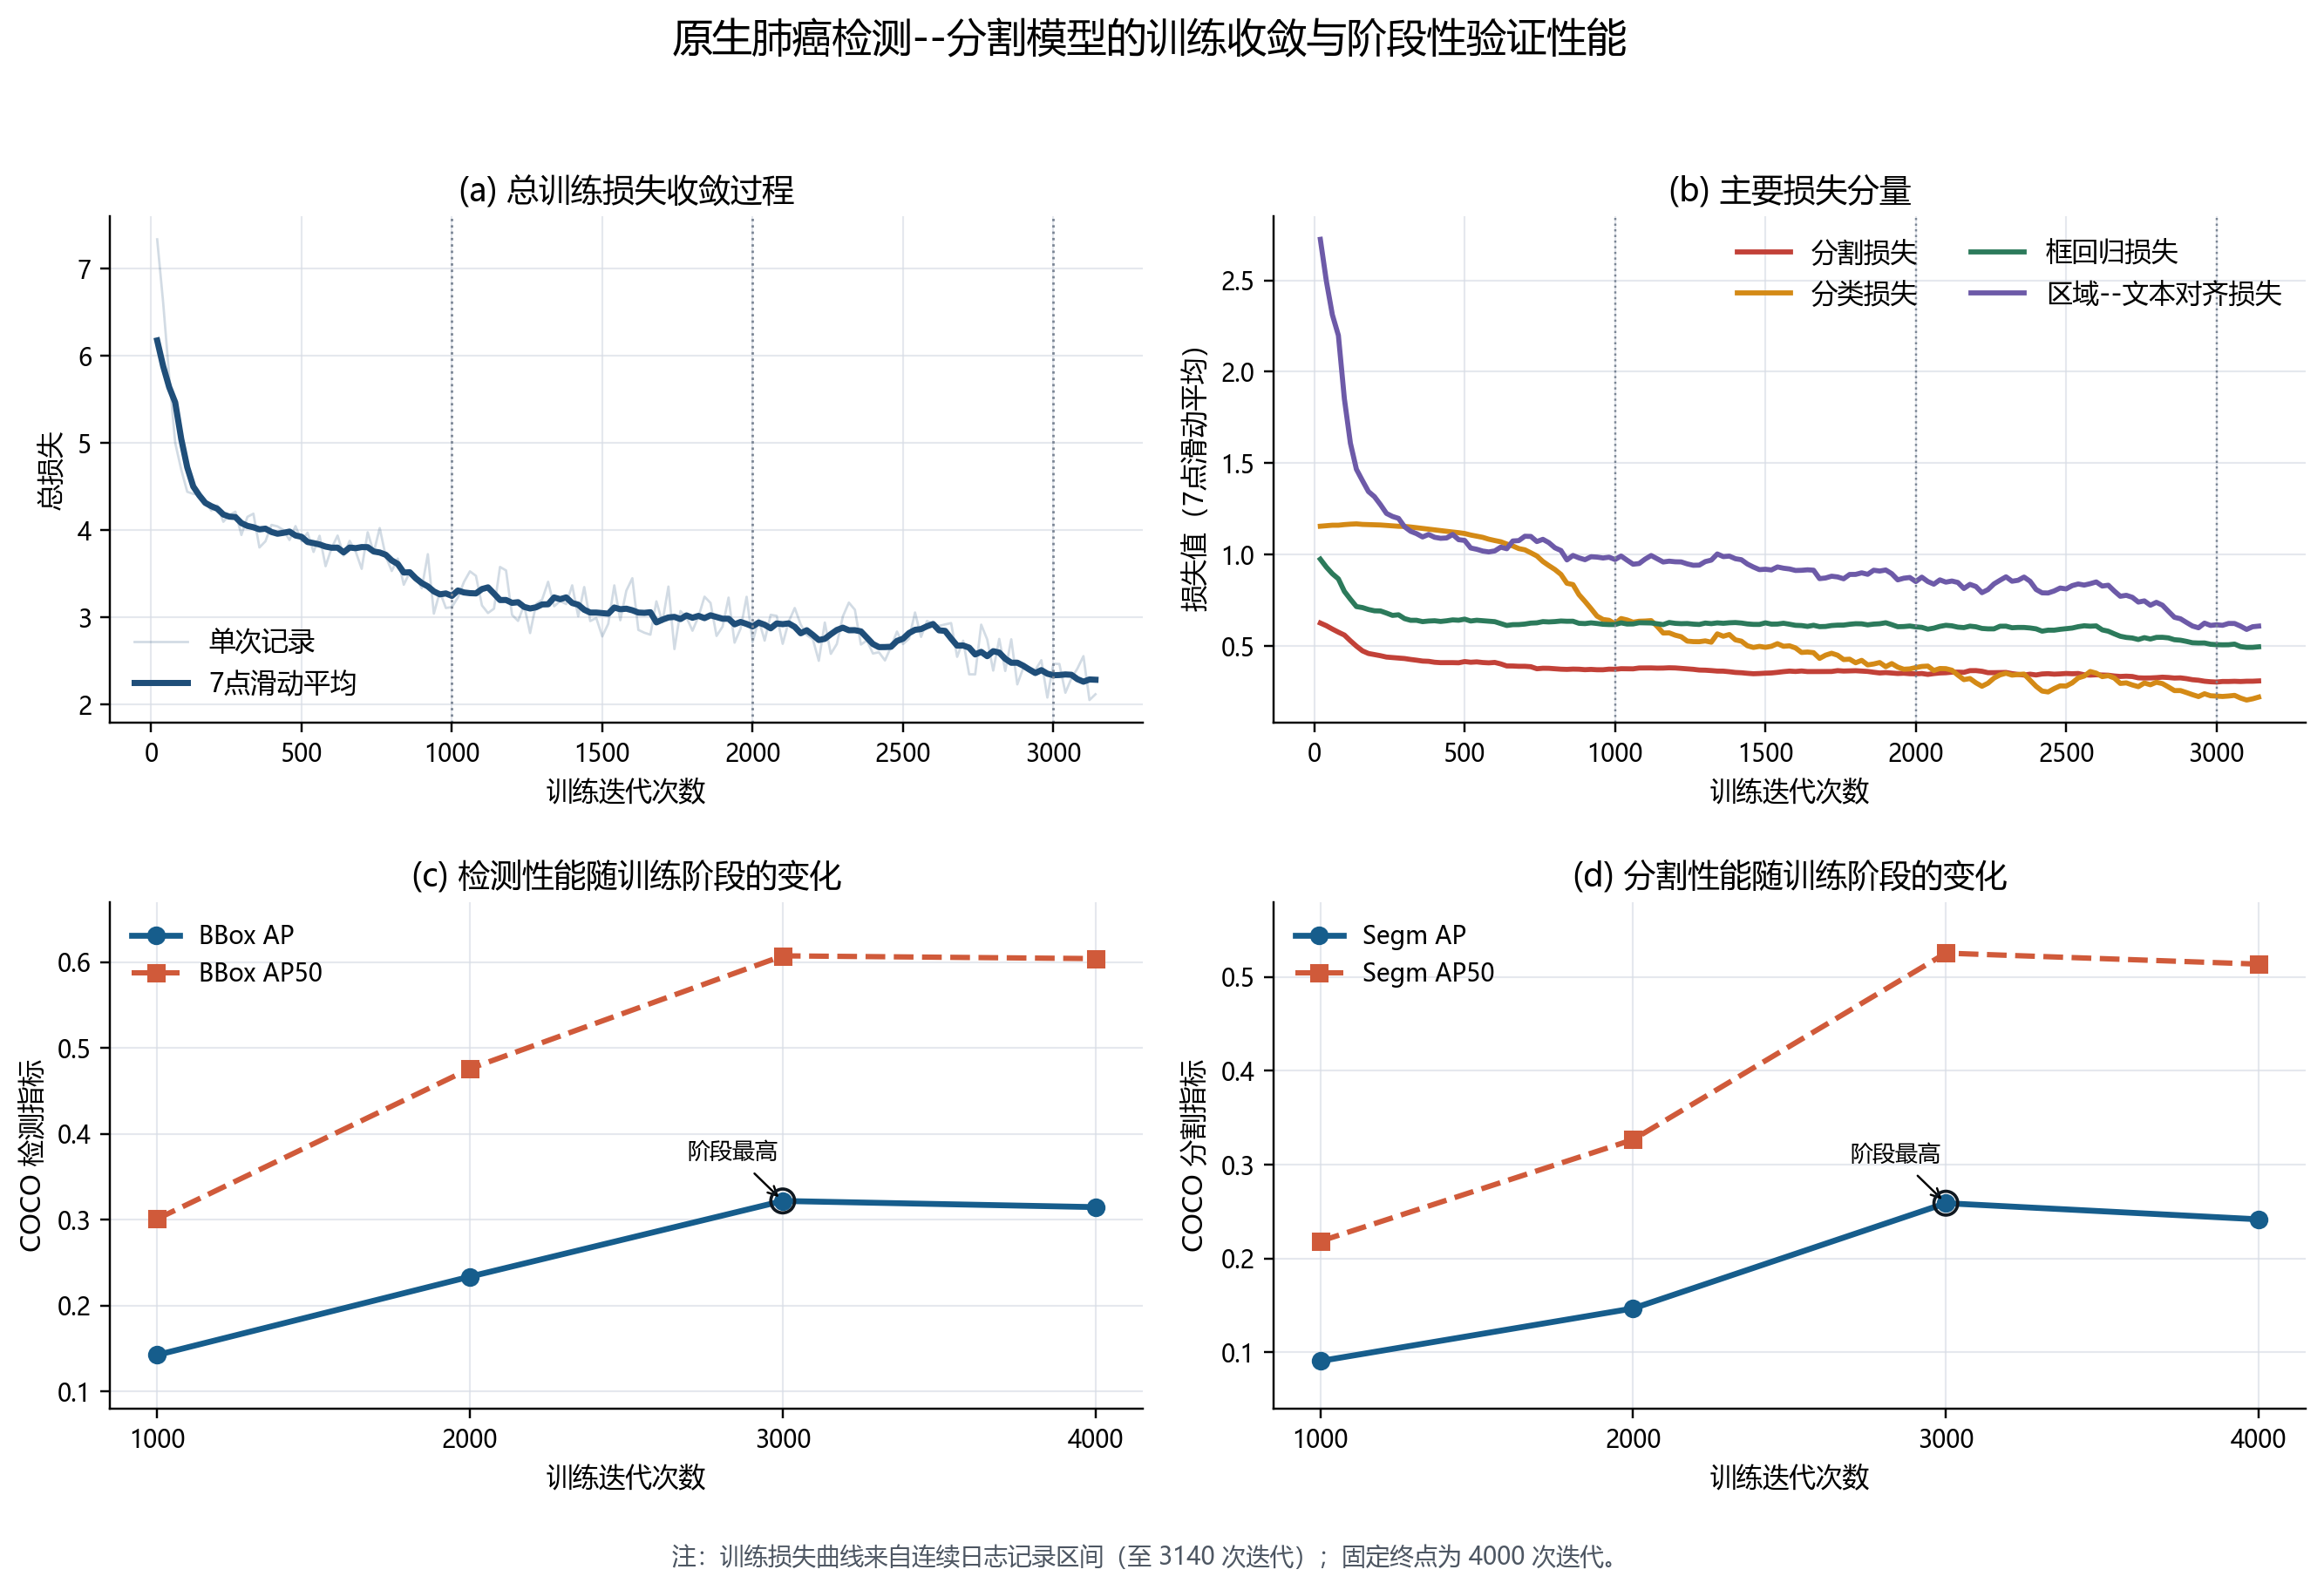
\includegraphics[width=0.96\textwidth]{chapters/lung_native_training_dynamics_20260901.png}
  \caption{原生肺癌检测--分割模型的训练收敛与阶段性性能}
  \label{fig:lung_native_segmentation_curve}
\end{figure}
图~\ref{fig:lung_native_segmentation_curve} 从优化过程和验证性能两个层面展示训练动态。（a）中总损失由训练初期的 6 以上持续下降至 3140 次迭代附近的约 2.3，原始记录虽存在小批量波动，7 点滑动平均曲线仍保持明确的下降趋势。（b）进一步分解主要损失项：区域--文本对齐损失在早期下降最快，分类损失在约 1000 次迭代后继续降低，框回归损失和分割损失则以较平缓的方式收敛。各分量均未出现持续发散或异常突增，说明检测分支、语言对齐分支与实例分割分支能够在联合训练中保持数值稳定。训练损失曲线依据当前保留的连续日志记录至 3140 次迭代，4000 次固定终点则由最终权重的独立评价结果确认。

图~\ref{fig:lung_native_segmentation_curve}（c）和（d）分别给出 1000、2000、3000 和 4000 次迭代时的检测与分割评价结果。检测 AP 从 0.142 提高至 3000 次迭代时的 0.322，分割 AP 同期由 0.091 提高至 0.259；4000 次迭代时两者分别轻微回落至 0.315 和 0.242，AP50 也呈现相同的先升高后轻微下降趋势。由此可见，训练损失继续降低并不必然带来验证集性能同步提高：模型在约 3000 次迭代后已接近小规模目标域数据上的泛化饱和点，继续训练可能强化对训练图块的拟合。为避免依据验证集事后挑选检查点，本文仍以预先规定的 4000 次迭代最终模型作为主结果，而将 3000 次迭代结果仅用于分析训练趋势。


\begin{figure}[tb]
  \centering
  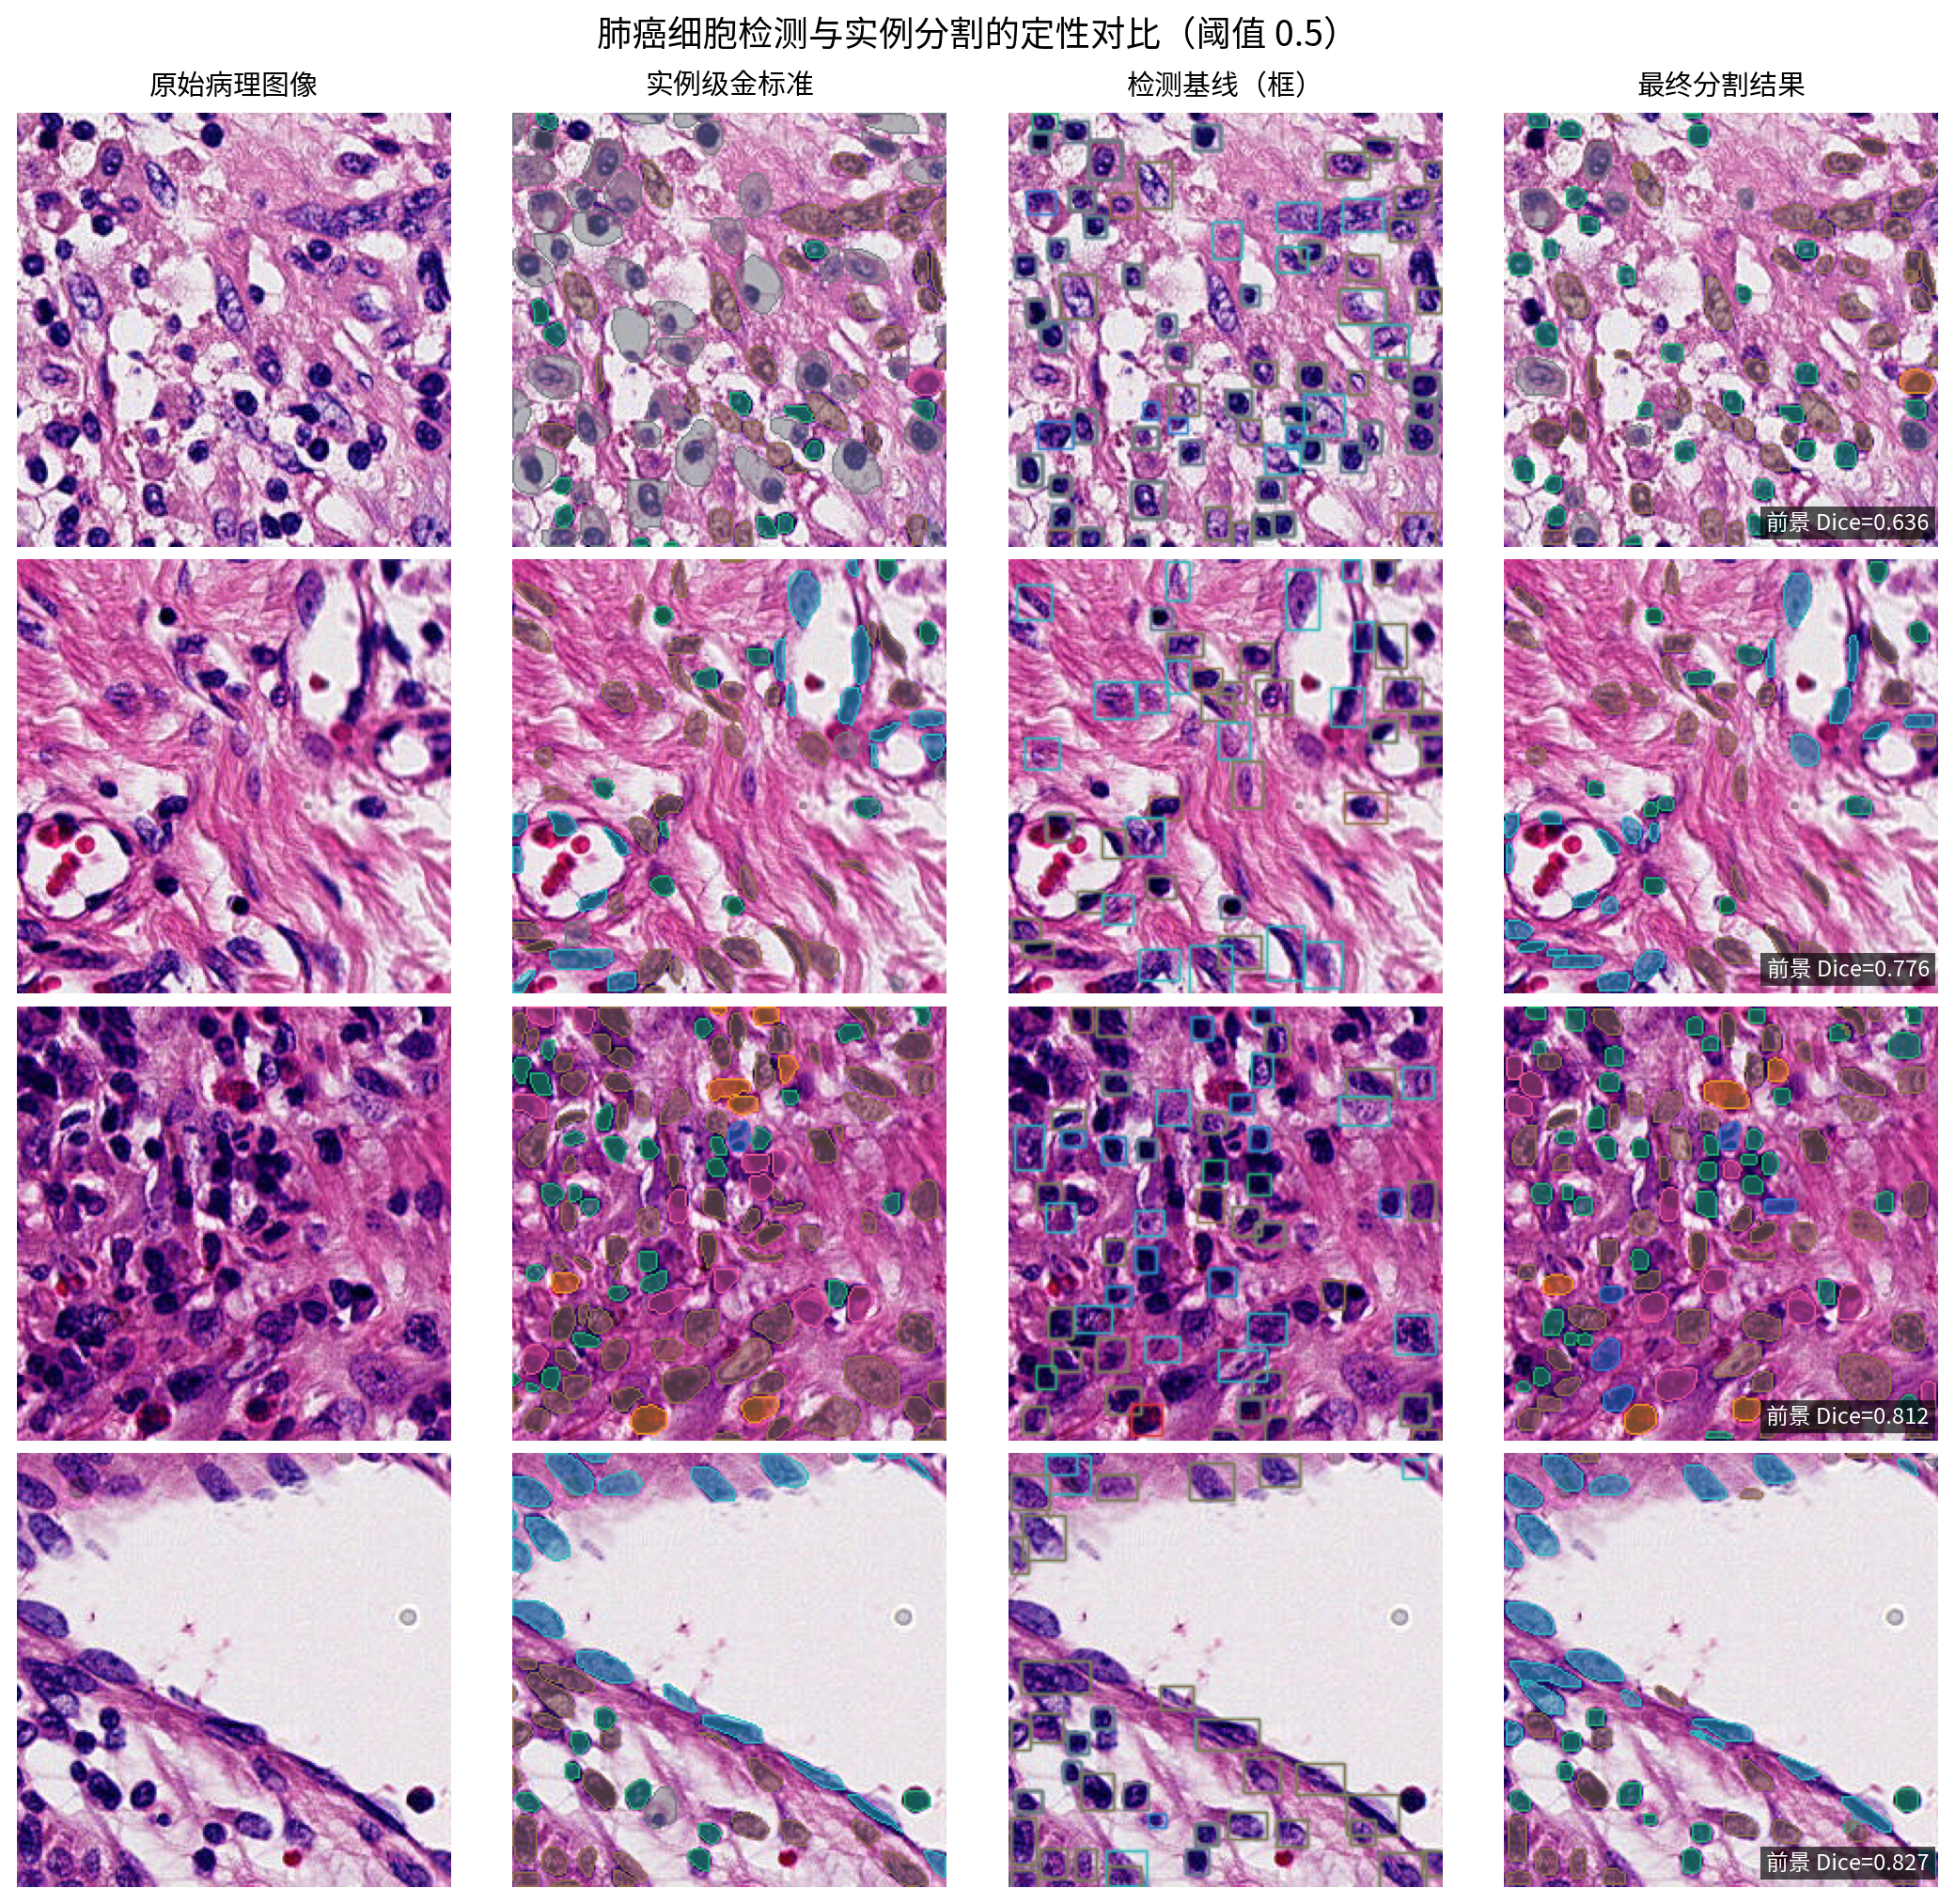
\includegraphics[width=0.92\textwidth]{chapters/lung_native_segmentation_final4000_4x4_20260901.png}
  \caption{肺癌细胞检测与实例分割的定性结果}
  \label{fig:lung_native_segmentation_final4000}
\end{figure}
图~\ref{fig:lung_native_segmentation_final4000} 按“原始病理图像--实例级金标准--历史检测基线--最终分割结果”四列展示代表性样本。样本依据前景 Dice 从低到高的分布位置选取，既包含较稳定案例，也保留一个相对困难案例。最终模型能够为肿瘤细胞、淋巴细胞、中性粒细胞和间质相关细胞等密集目标生成独立轮廓，较框级输出提供了更细的形态信息；但在细胞拥挤、边界模糊和切片边缘区域仍可见漏分、粘连或轮廓偏移。图中 Dice 为阈值 0.5 下的图块级前景 Dice，用于说明轮廓覆盖情况，不等同于按类别汇总的 COCO Segm AP。

上述结果仍需结合数据规模理解。当前评价集只有 8 个图块，虽然已核查训练集与评价集之间不存在同名文件或完全相同的图像哈希，但在缺少完整临床病例清单的情况下，尚不能据此宣称严格的患者级独立。后续应在具有明确患者标识的外部队列上扩大样本量，统一嗜酸性粒细胞相关标签，并报告患者分层的置信区间，才能更充分评价联合检测--分割模型的泛化能力。


\subsection{AI-RVT 与 VIS-RVT 的一致性}
在 SXCH 外部验证队列中，AI-RVT 与 VIS-RVT 的切片级组内相关系数（intraclass correlation coefficient, ICC）为 0.881（$p=1.08\times10^{-64}$），患者级 ICC 为 0.861（$p=6.03\times10^{-10}$）。在 NCC\_Cohort2 与 SZCH 组成的独立测试数据中，切片级 ICC 为 0.861（$p=6.96\times10^{-273}$），患者级 ICC 进一步达到 0.931（$p=1.05\times10^{-38}$）。患者级聚合降低了单张切片取材差异的影响，因而获得了更稳定的一致性。

采用 10\% RVT 阈值划分 MPR 和 non-MPR 时，AI-RVT 与 VIS-RVT 在 84 例患者中的一致率为 95.2\%（80/84）。四例不一致病例中，t1、t3 和 t4 均位于 10\% 阈值附近，主要反映边界病例的连续值差异；t2 的 VIS-RVT 为 22\%，AI-RVT 为 8.56\%，高倍图像显示活性肿瘤与间质广泛交织，人工视觉评估可能因复杂间质结构而高估活性肿瘤比例。该结果同时说明，连续 RVT 比单一阈值标签保留了更多病理信息。

\begin{figure}[tb]
  \centering
  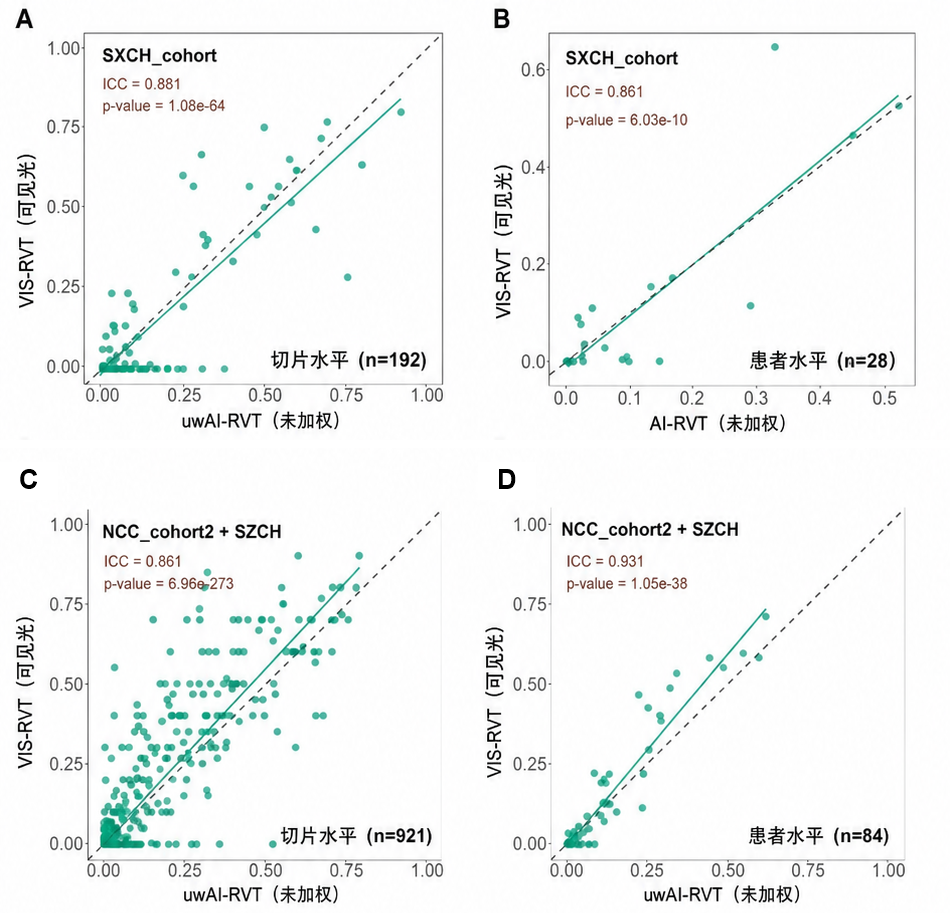
\includegraphics[width=0.70\textwidth]{chapters/lung_fig5_5_abef_precise_abcd_20260829.png}
  \caption{AI-RVT 与 VIS-RVT 的跨队列一致性}
  \label{fig:lung_concordance_quant}
\end{figure}
图~\ref{fig:lung_concordance_quant} 集中展示跨中心定量一致性。（A、B）分别为 SXCH 外部验证队列的切片级和患者级结果，ICC 为 0.881 和 0.861；（C、D）在 NCC\_Cohort2 与 SZCH 独立测试数据中重复评价，ICC 分别为 0.861 和 0.931。患者级聚合后仍保持较高一致性，说明模型并非只在个别切片上偶然吻合；相反，汇总同一患者多张 WSI 能够降低取材位置和局部异质性引起的波动。两组独立队列得到相近结论，也为 AI-RVT 的跨中心稳定性提供了证据。

\begin{figure}[tb]
  \centering
  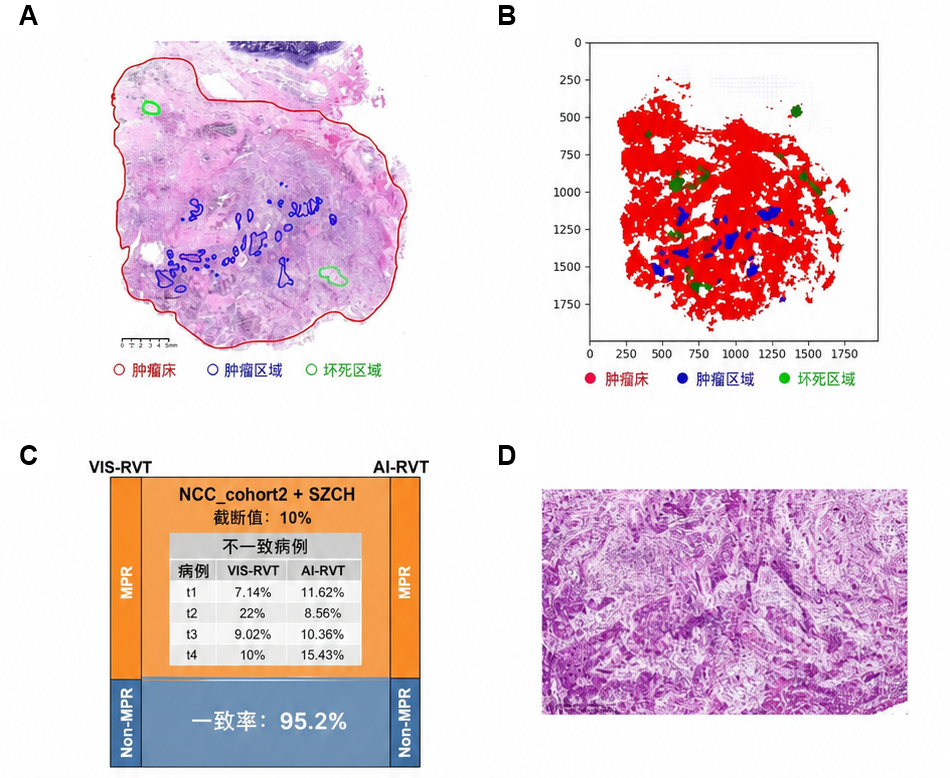
\includegraphics[width=0.72\textwidth]{chapters/lung_fig5_5_cdgh_precise_abcd_20260829.png}
  \caption{区域分割对照与 MPR 阈值判定}
  \label{fig:lung_concordance_cases}
\end{figure}
图~\ref{fig:lung_concordance_cases} 进一步解释一致性结果的病理来源。（A、B）将病理医师勾画的肿瘤床、活性肿瘤和坏死区域与 AI 分割结果并列，可见主体区域的空间判断总体一致，而差异主要位于复杂边界。（C）在 10\% RVT 阈值下比较 MPR 判定，84 例患者中有 80 例结论一致，一致率为 95.2\%。（D）展示差异较明显的病例：活性肿瘤与纤维化间质广泛交错，人工视觉估计容易受到局部高细胞密度区域影响。该病例说明，连续 AI-RVT 可保留阈值附近的细微差异，但不一致病例仍应结合原始 H\&E 形态复核。

\subsection{预后分析结果}
\subsubsection{阈值化 MPR 分层}
在 103 例总体预后队列中，VIS-RVT 和 AI-RVT 定义的 MPR 均能显著区分 DFS，log-rank 检验的 $p$ 值分别为 0.0011 和 0.00095。校正 ypN 后，VIS-RVT 定义的 non-MPR 风险比为 2.6（95\% CI：1.09--6.20，$p=0.031$），AI-RVT 定义的 non-MPR 风险比为 2.7（95\% CI：1.18--6.40，$p=0.019$）。两种方法对 OS 的分层均未达到显著水平，其中 VIS-RVT 的 $p=0.33$，AI-RVT 呈非显著趋势（$p=0.084$）。

在 78 例 non-pCR 亚组中，VIS-RVT 和 AI-RVT 定义的 MPR 仍能区分 DFS，$p$ 值分别为 0.023 和 0.021。多变量模型中，VIS-RVT 仅呈边界显著（HR=2.3，$p=0.061$），而 AI-RVT 定义的 non-MPR 仍与较短 DFS 独立相关（HR=2.5，95\% CI：1.04--6.0，$p=0.040$）。这一差异表明，自动化区域量化在残余肿瘤患者中可能比阈值化人工估计具有更稳定的风险识别能力。

\subsubsection{连续 RVT 分析}
将 RVT 作为连续变量可避免 10\% 阈值造成的信息损失。在总体队列中，连续 VIS-RVT 与 AI-RVT 的 DFS 风险比分别为 8.4（$p=0.009$）和 8.2（$p=0.022$）；在 non-pCR 亚组中，两者的风险比分别为 7.2（$p=0.018$）和 7.0（$p=0.037$）。二者效应方向和量级高度一致，但均未对 OS 显示稳定关联。这表明 RVT 更直接反映复发风险，而 OS 可能同时受到后续治疗、非肿瘤死亡和治疗后免疫生态等因素影响。

\begin{figure}[tb]
  \centering
  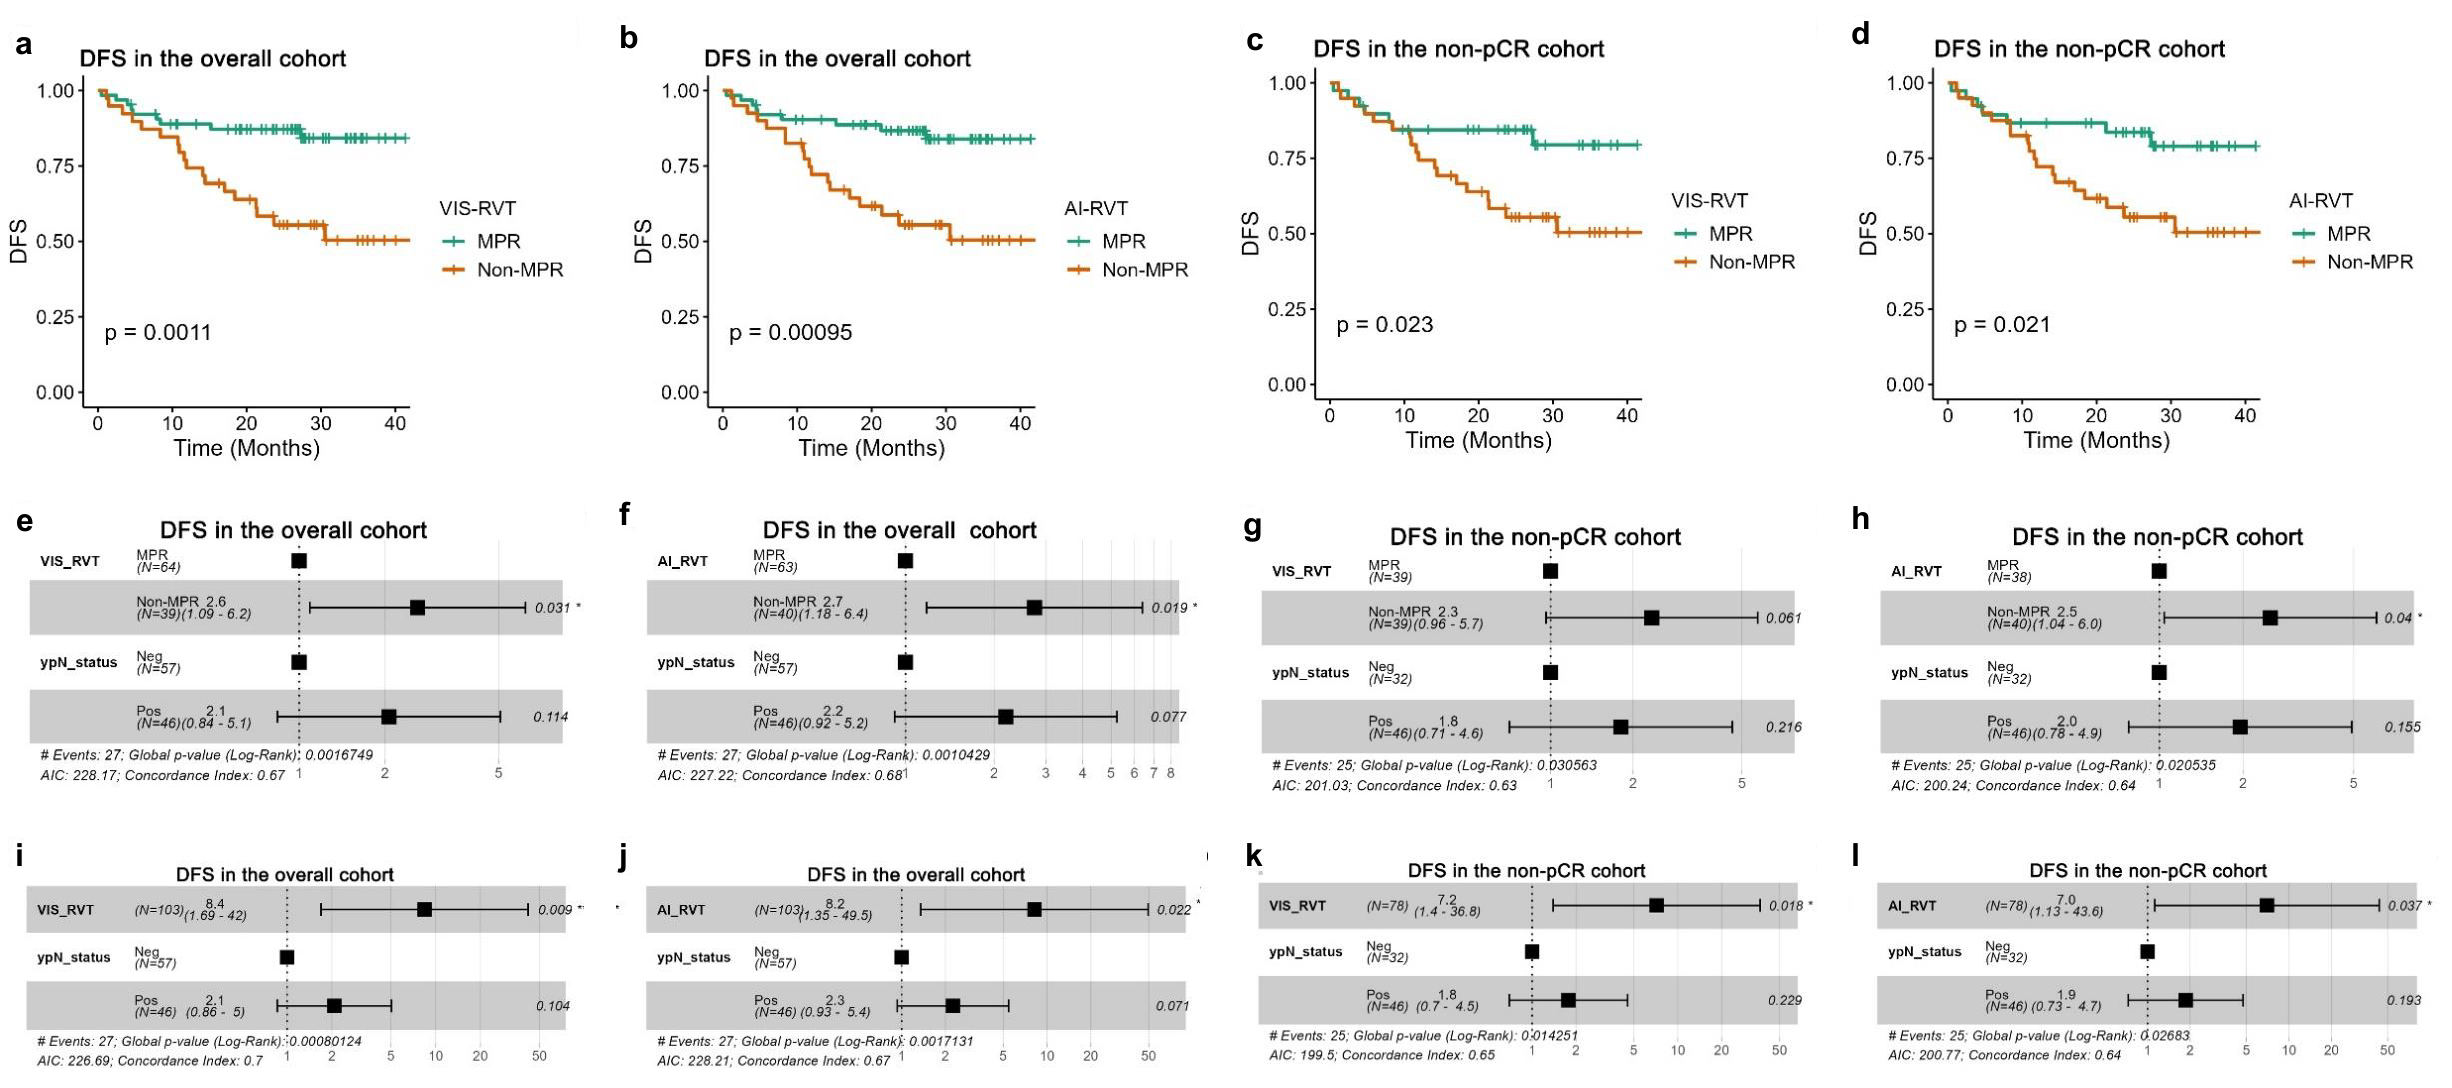
\includegraphics[width=\textwidth]{chapters/lung_rvt_survival_3x4_20260831.png}
  \caption{RVT 与无病生存期的关联}
  \label{fig:lung_rvt_survival}
\end{figure}
图~\ref{fig:lung_rvt_survival} 从阈值分层和连续变量两个角度说明 RVT 与无病生存期的关系。第一行（a--d）给出 Kaplan--Meier 曲线：（a、b）分别采用 VIS-RVT 与 AI-RVT，在总体队列中划分 MPR 和 non-MPR；（c、d）则将同样的分析限制在 non-pCR 患者中，以排除完全缓解病例对结果的主导作用。四幅曲线均显示 non-MPR 患者的 DFS 较差，说明两种 RVT 评估均可形成与临床结局相关的患者分层。

第二行（e--h）对应多变量 Cox 分析，其中（e、f）为总体队列，（g、h）为 non-pCR 亚组。在校正 ypN 等临床因素后，总体队列中两种 RVT 定义仍保留独立的 DFS 风险信息，AI-RVT 定义的 non-MPR 风险比为 2.7。在 non-pCR 亚组中，VIS-RVT 的关联减弱，而 AI-RVT 的关联仍达到统计学显著。该结果支持自动量化评估具有一定的预后分层价值，但不能仅依据生存关联直接推断其测量重复性。

第三行（i--l）不再使用 10\% 二分阈值，而是直接把 RVT 作为连续变量进入模型；（i、j）分析总体队列，（k、l）分析 non-pCR 亚组。两种评估在不同人群中的效应方向保持一致。连续分析保留了治疗反应程度的梯度信息，避免将 9\% 与 11\% 这类数值接近的病例仅按阈值分到不同组，可作为 MPR 分层分析的补充。

\subsection{空间免疫分析结果}
\subsubsection{距离依赖的单一细胞效应}
在具有残余肿瘤的 NCC 和 SZCH 患者中，$50$--$700\,\mu\mathrm{m}$ 各距离范围的细胞组成总体一致：成纤维细胞最丰富，其次为淋巴细胞；浆细胞、组织细胞、中性粒细胞和内皮细胞处于中等水平；嗜酸性粒细胞因数量过少而不纳入预后分析。

既往研究已表明，肿瘤免疫微环境不仅取决于细胞丰度，还取决于免疫细胞的空间组织、细胞邻域和浸润形态\cite{keren2018structured,saltz2018spatial}；在早期非小细胞肺癌中，TIL 的空间结构亦与复发风险相关\cite{corredor2019spatil}。空间 Cox 分析显示，不同细胞的预后作用具有明确的距离依赖性。对于 DFS，肿瘤边界 $50\,\mu\mathrm{m}$ 内高中性粒细胞密度与较差 DFS 相关（log-rank $p=0.040$），同一区域高内皮细胞密度也与较差 DFS 相关（$p=0.014$）。同时纳入 ypN 和 AI-RVT 后，内皮细胞密度仍是独立复发风险因素（HR=2.9，95\% CI：1.07--7.8，$p=0.036$），而中性粒细胞对 DFS 不再独立显著。

OS 呈现另一组互补信号。$50\,\mu\mathrm{m}$ 内高中性粒细胞密度与较差 OS 相关（log-rank $p=0.0089$），$700\,\mu\mathrm{m}$ 范围内高淋巴细胞密度则与更好 OS 相关（$p=0.032$）。在校正 ypN 和 AI-RVT 的 Firth Cox 模型中，远端淋巴细胞仍是保护因素（HR=0.15，95\% CI：0.015--0.79，$p=0.024$），近端中性粒细胞则是风险因素（HR=7.5，95\% CI：1.5--76，$p=0.012$）。这说明紧邻肿瘤的中性粒细胞富集和更广空间内的淋巴细胞浸润分别刻画局部不利炎症生态与整体抗肿瘤免疫能力。

\begin{table}[htbp]
  \centering
  \caption{空间免疫特征的预后效应}
  \label{tab:lung_spatial_effects}
  \resizebox{0.98\textwidth}{!}{%
  \begin{tabular}{lllll}
    \toprule
    终点 & 空间特征 & 单因素 $p$ 值 & 多变量 HR（95\% CI） & 多变量 $p$ 值 \\
    \midrule
    DFS & 中性粒细胞，$50\,\mu\mathrm{m}$ & 0.040 & 1.2（0.47--3.3） & 0.663 \\
    DFS & 内皮细胞，$50\,\mu\mathrm{m}$ & 0.014 & 2.9（1.07--7.8） & 0.036 \\
    OS & 中性粒细胞，$50\,\mu\mathrm{m}$ & 0.0089 & 7.5（1.5--76） & 0.012 \\
    OS & 淋巴细胞，$700\,\mu\mathrm{m}$ & 0.032 & 0.15（0.015--0.79） & 0.024 \\
    \bottomrule
  \end{tabular}}
\end{table}

\begin{figure}[tb]
  \centering
  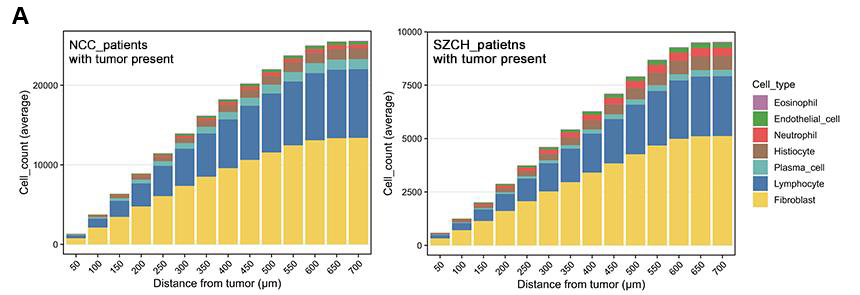
\includegraphics[width=0.82\textwidth]{chapters/lung_fig5_7_a_precise_A_20260829.png}
  \caption{跨中心不同径向范围的细胞组成}
  \label{fig:lung_spatial_composition}
\end{figure}
图~\ref{fig:lung_spatial_composition} 首先比较 NCC 与 SZCH 残余肿瘤患者在 $50$--$700\,\mu\mathrm{m}$ 径向范围内的累积细胞组成。两队列随距离增加呈现相近的总体趋势，成纤维细胞和淋巴细胞占比较高，中性粒细胞、内皮细胞等类别所占比例较低但具有特定空间分布。跨中心组成的一致性说明，后续预后关联并非由某一个中心特有的细胞构成所驱动；同时，累计数量随距离增加并不意味着风险效应同步增强，真正具有解释价值的是细胞类别、肿瘤距离和临床终点三者的联合关系。

\begin{figure}[tb]
  \centering
  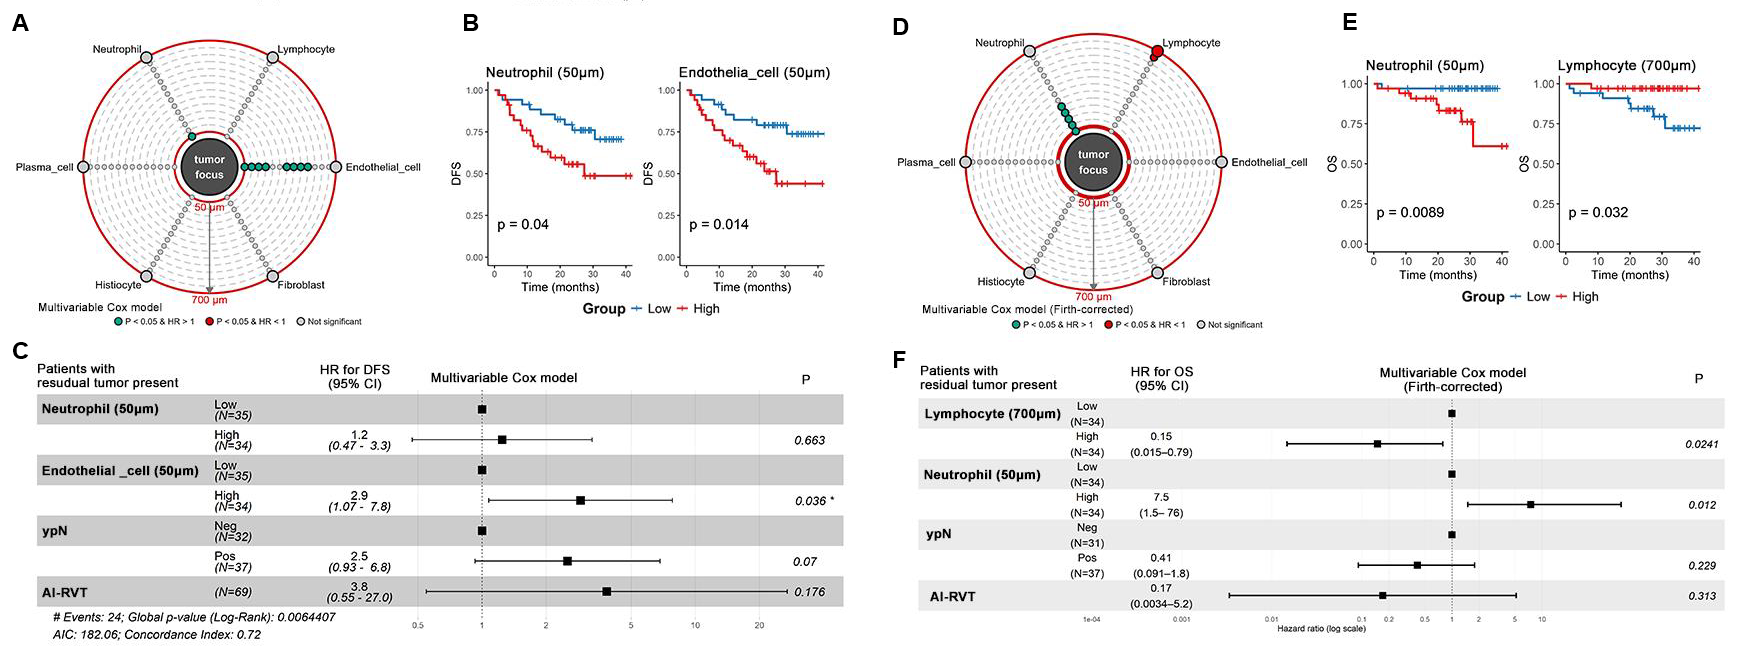
\includegraphics[width=\textwidth]{chapters/lung_spatial_survival_horizontal_20260831.png}
  \caption{空间免疫特征与生存结局}
  \label{fig:lung_spatial_survival}
\end{figure}
图~\ref{fig:lung_spatial_survival} 将距离扫描结果与生存分析对应起来。左侧（A--C）聚焦 DFS：径向扫描提示肿瘤边界近端的中性粒细胞和内皮细胞与较差结局相关，Kaplan--Meier 曲线展示高低密度组差异，多变量模型进一步校正 ypN 与 AI-RVT。校正后，$50\,\mu\mathrm{m}$ 内内皮细胞仍保持独立风险作用（HR=2.9，$p=0.036$），而中性粒细胞的 DFS 效应减弱。右侧（D--F）采用同样结构分析 OS，并针对较少事件使用 Firth 校正。$50\,\mu\mathrm{m}$ 内高中性粒细胞密度是风险因素（HR=7.5，$p=0.012$），$700\,\mu\mathrm{m}$ 内高淋巴细胞密度则表现为保护因素（HR=0.15，$p=0.024$）。结果说明，紧邻肿瘤的局部促肿瘤炎症与更大范围的抗肿瘤免疫浸润是方向相反但可同时存在的空间生态。

\subsubsection{淋巴细胞--中性粒细胞联合表型}
根据 $700\,\mu\mathrm{m}$ 内淋巴细胞密度和 $50\,\mu\mathrm{m}$ 内中性粒细胞密度，将残余肿瘤患者划分为四种 Lym+Neu 空间免疫表型。联合表型能够区分 DFS（log-rank $p=0.026$）：低淋巴细胞/高中性粒细胞组的 DFS 最差，高淋巴细胞/低中性粒细胞组最好；但该 DFS 关联在多变量模型中未保持独立显著。

相比之下，联合表型对 OS 的区分更强（log-rank $p=0.0092$）。在校正 ypN 和 AI-RVT 的 Firth Cox 模型中，低淋巴细胞/高中性粒细胞表型相对于高淋巴细胞/低中性粒细胞表型仍与不良 OS 独立相关，HR 为 31（95\% CI：3.2--402，$p=0.0011$）。较宽的置信区间反映 OS 事件数有限，但效应方向与单一细胞分析完全一致：近端中性粒细胞富集与远端淋巴细胞缺失共同构成最不利的治疗后免疫结构。

\begin{figure}[tb]
  \centering
  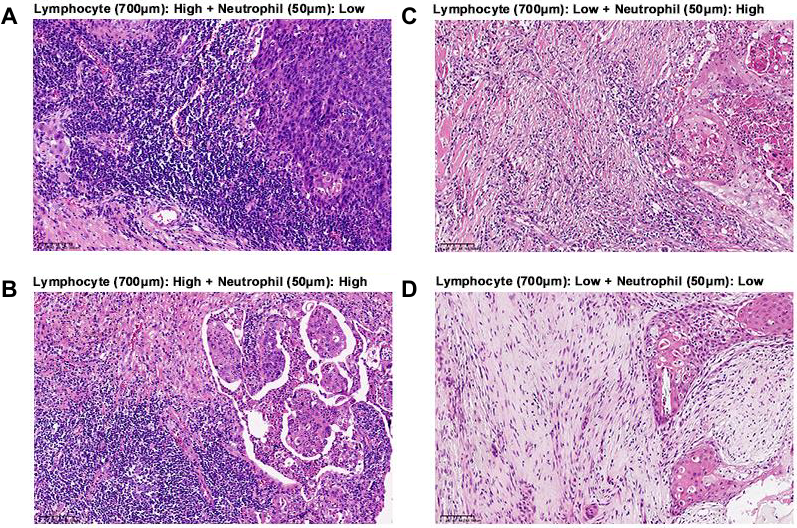
\includegraphics[width=0.92\textwidth]{chapters/lung_combined_morphology_rotated_20260831.png}
  \caption{淋巴细胞--中性粒细胞联合表型的病理形态}
  \label{fig:lung_combined_morphology}
\end{figure}
图~\ref{fig:lung_combined_morphology} 展示四种联合表型的代表性 H\&E 区域。左列依次为（A）高淋巴细胞/低中性粒细胞和（B）高淋巴细胞/高中性粒细胞，右列依次为（C）低淋巴细胞/高中性粒细胞和（D）低淋巴细胞/低中性粒细胞。这里的“高/低”分别依据 $700\,\mu\mathrm{m}$ 范围内的淋巴细胞密度与 $50\,\mu\mathrm{m}$ 范围内的中性粒细胞密度定义，并非仅凭所展示的局部视野判断。该划分同时编码较大范围的适应性免疫浸润和紧邻肿瘤的炎症反应，比单独统计某一类细胞更接近真实肿瘤微环境。

\begin{figure}[tb]
  \centering
  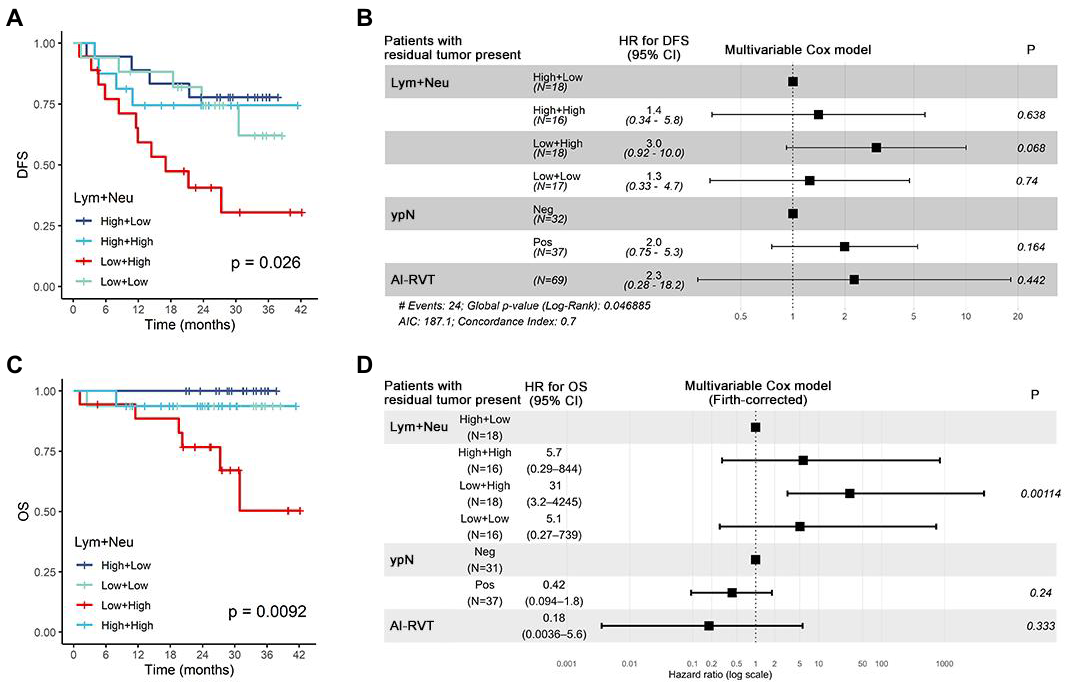
\includegraphics[width=0.95\textwidth]{chapters/lung_combined_survival_abcd_20260831.png}
  \caption{淋巴细胞--中性粒细胞联合表型与生存结局}
  \label{fig:lung_combined}
\end{figure}
图~\ref{fig:lung_combined} 分析上述四种联合表型与生存结局的关系。（A、B）显示联合表型能够区分 DFS，其中低淋巴/高中性组曲线最差、高淋巴/低中性组最好；校正临床变量后，DFS 关联减弱，说明复发风险仍较多受到残余肿瘤负荷和淋巴结状态影响。（C、D）显示联合表型对 OS 的分层更明显。在 Firth 校正模型中，低淋巴/高中性组相对于高淋巴/低中性组仍具有显著较高风险，方向与图~\ref{fig:lung_spatial_survival} 的单细胞结果一致。由于 OS 事件数有限、置信区间较宽，该结果更适合作为具有生物学一致性的风险信号，仍需在更大规模前瞻性队列中验证。

\subsection{细胞实例特征分布分析}
为检验渐进式视觉语言预训练是否改善肺鳞癌病理细胞的实例表征，本文对同一批标注实例分别提取未经额外医学预训练的 GLIP-ZS 特征与渐进式预训练后的特征，并采用一致的 PCA 与 t-SNE 参数进行降维。参与比较的类别包括肿瘤细胞、淋巴细胞、中性粒细胞、浆细胞、血管内皮细胞和纤维间质细胞等。

\begin{figure}[tb]
  \centering  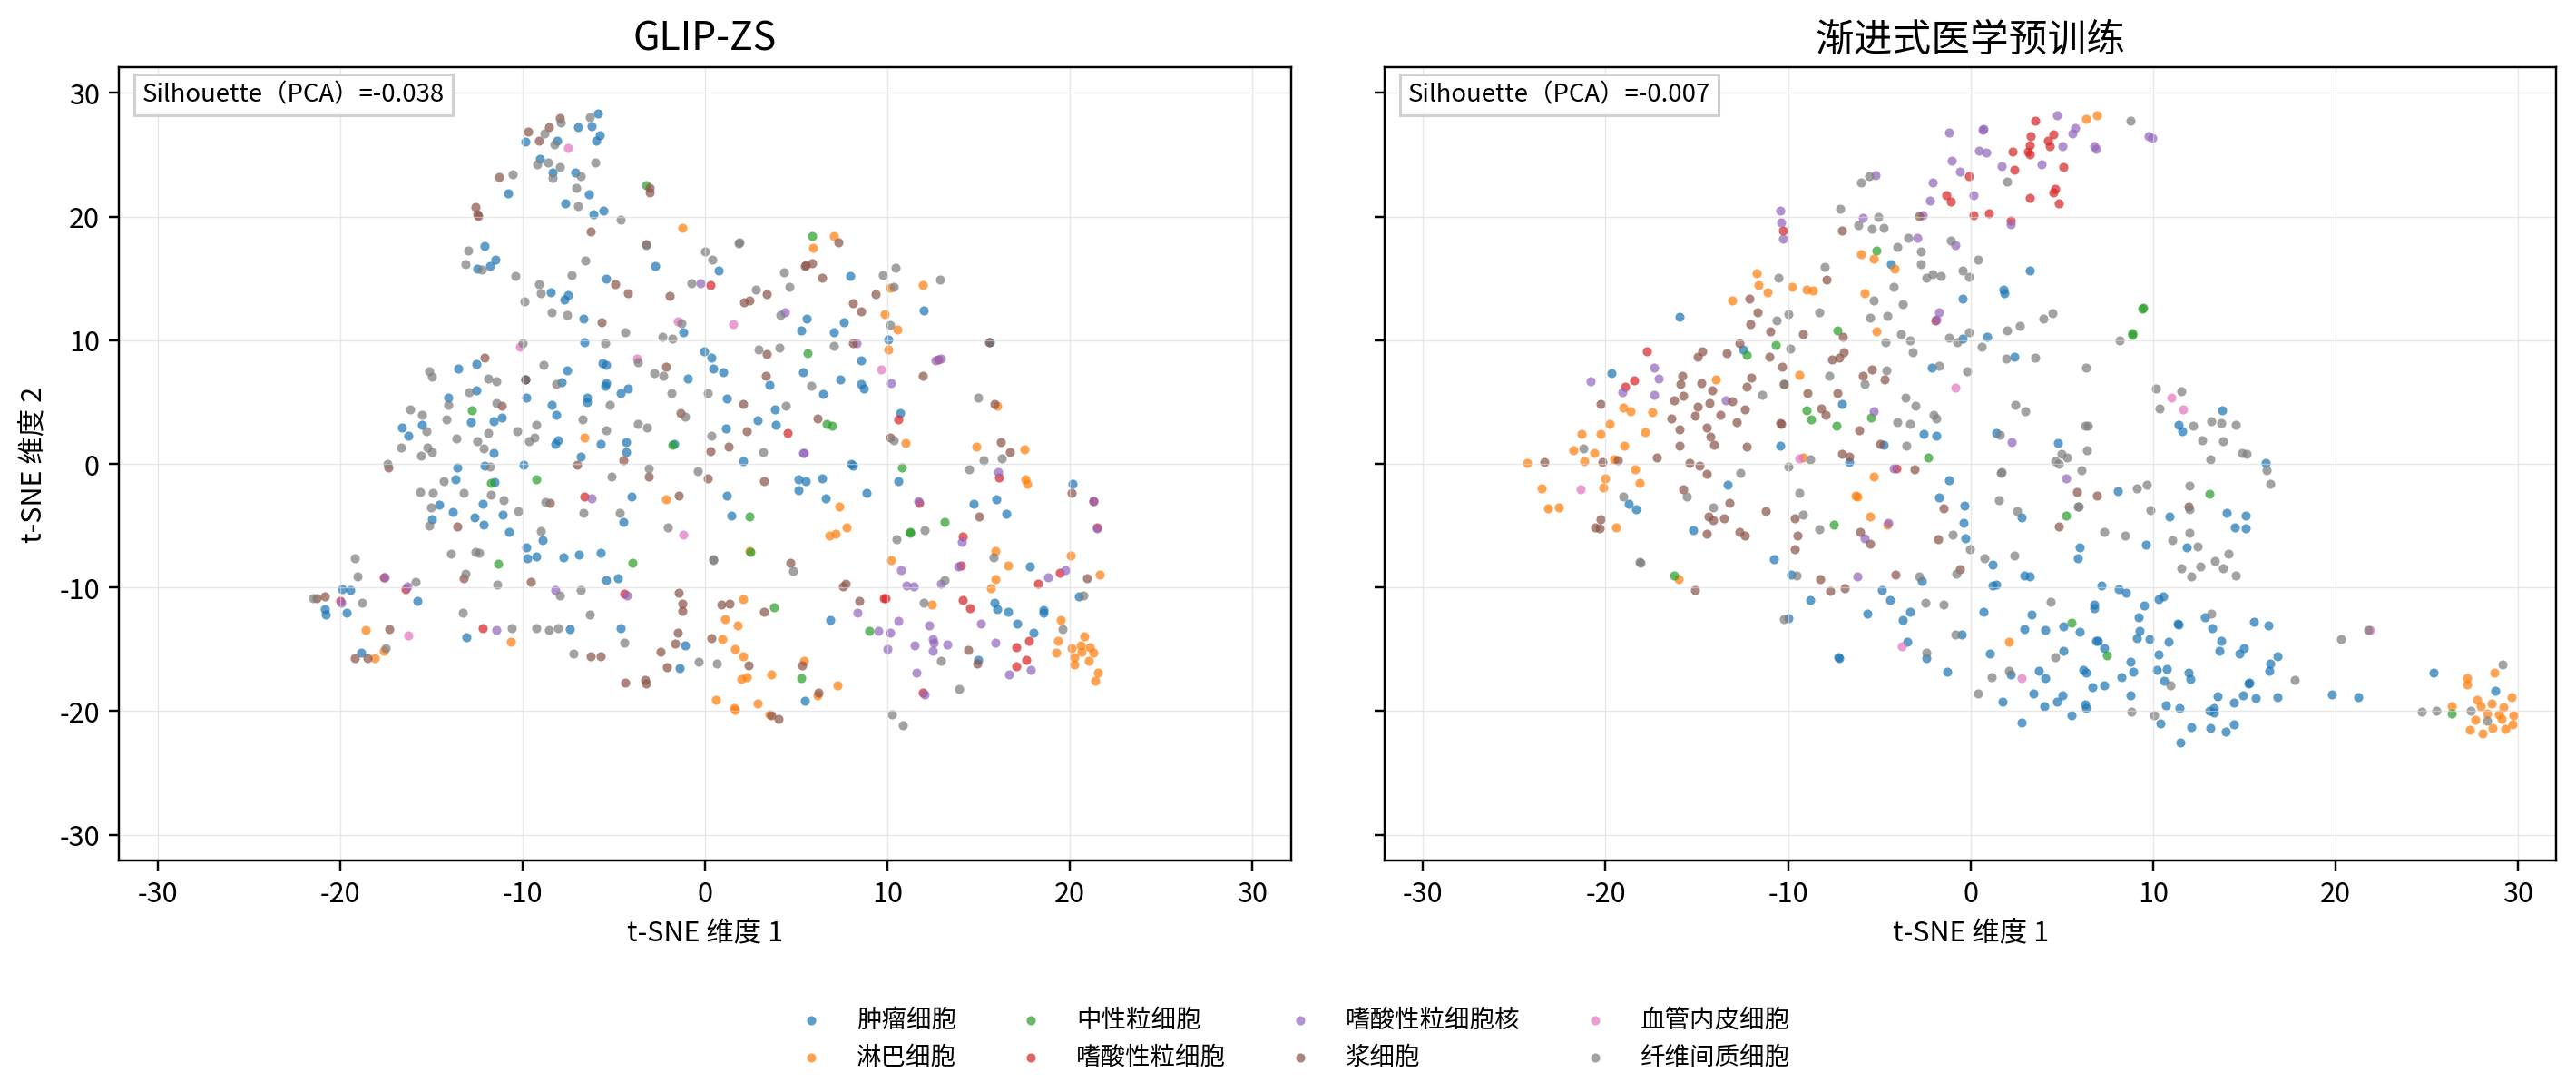
\includegraphics[width=0.84\textwidth]{figures/figure5_lungscc_tsne_centered_20260823.png}  \caption{GLIP-ZS 与渐进式预训练模型的肺鳞癌细胞实例特征分布}  \label{fig:lung_progressive_tsne}
\end{figure}
图~\ref{fig:lung_progressive_tsne} 显示，渐进式预训练后同类样本的局部聚集趋势更加明显，PCA 特征上的轮廓系数由 $-0.038$ 提高至 $-0.007$，t-SNE 平面上的轮廓系数由 $-0.149$ 提高至 $-0.056$。指标仍为负值，说明不同细胞形态之间依然存在较强重叠，因此该结果应理解为可分性的相对改善，而不是类别已经完全分离。左右子图仅通过二维平移进行显示居中，样本间距离和评价指标均未改变。

\section{本章小结}
本研究将治疗后 LUSC 的病理分析拆分为三个相互衔接且可解释的层次。第一层通过多尺度区域分类量化 RVT，解决人工估计工作量大和重复性不足的问题；第二层利用视觉语言基础模型统一异构细胞标签空间，在有限域内标注下识别七类肿瘤周围非肿瘤细胞；第三层将细胞位置转换为相对肿瘤边界的空间密度，以解释具有相似 RVT 患者之间仍然存在的预后差异。

AI-RVT 在外部验证和独立测试数据中均与 VIS-RVT 高度一致，患者级 ICC 达到 0.861--0.931，10\% 阈值下的一致率为 95.2\%。更重要的是，AI-RVT 的价值不仅是复现病理医师的读数。在 non-pCR 人群中，AI-RVT 定义的 non-MPR 在校正 ypN 后仍能独立预测 DFS，而 VIS-RVT 仅达到边界显著。连续 RVT 的风险效应又明显强于简单的 MPR 二分，说明治疗反应本质上是连续谱，强制阈值化会损失临床相关信息。

RVT 对 DFS 的稳定作用和空间免疫特征对 OS 的补充作用具有生物学合理性。RVT 更直接反映新辅助治疗后的局部肿瘤清除程度，因此首先关联复发；OS 则受到宿主免疫状态、后续治疗及全身疾病过程的共同影响。近端中性粒细胞富集可能对应免疫抑制、组织损伤和促肿瘤炎症，远端淋巴细胞丰富则更可能反映广泛而持续的抗肿瘤免疫。将两者组合后，低淋巴细胞/高中性粒细胞表型在校正 AI-RVT 与 ypN 后仍显示最高 OS 风险，说明空间免疫表型能够提供超越残余肿瘤负荷的互补信息。

本研究仍存在若干限制。首先，研究为回顾性设计，OS 事件数较少，尽管采用 Firth 校正降低了估计偏倚，HR=31 的置信区间仍较宽，需要更大规模前瞻性多中心队列验证。其次，每张 WSI 以最大肿瘤灶代表周边微环境，尚未完全覆盖多灶和区域异质性。再次，细胞类别依据 H\&E 形态预测，不能替代免疫组化或空间组学对功能亚型的鉴定。最后，当前方法主要计算到肿瘤边界的径向距离，后续可进一步引入细胞邻接图、聚集结构和三级淋巴结构等高阶空间特征。

本章的创新主要体现在以下三个方面。

第一，提出模拟病理医师“器官--组织--细胞”阅片过程的多尺度 WSI 模型，通过空间对齐的感受野扩展和面积加权融合生成连续 AI-RVT，在外部与独立数据中实现稳定的患者级一致性。

第二，提出面向异构病理细胞数据的渐进式视觉语言预训练策略，将公共多类核数据、目标域肿瘤/间质粗标注及少量八类精细标注依次用于域适配，在相同流程下显著优于 Mask R-CNN 和未经额外预训练的 GLIP。

第三，建立以肿瘤边界为参照的 $50$--$700\,\mu\mathrm{m}$ 空间免疫量化方法，发现近端中性粒细胞和远端淋巴细胞具有方向相反的 OS 效应，并构建能够在校正 AI-RVT 与 ypN 后继续分层 OS 的 Lym+Neu 联合表型。

本章围绕肺鳞癌新辅助免疫化疗后的疗效与预后评估，形成了“多尺度区域识别--连续 AI-RVT--多类细胞检测--空间密度建模--联合生存分析”的完整技术链。终稿结果表明，AI-RVT 能够高一致性复现人工 RVT，并对总体及 non-pCR 人群的 DFS 提供稳定信息；空间免疫分析进一步揭示 $50\,\mu\mathrm{m}$ 近端中性粒细胞的风险作用和 $700\,\mu\mathrm{m}$ 远端淋巴细胞的保护作用。二者构成的低淋巴细胞/高中性粒细胞表型识别出残余肿瘤患者中 OS 最差的亚群，从而把自动病理反应评估扩展为可解释的术后风险分层框架。

\chapter{统一实验设置、指标体系与复现细节}

\section{本章写作目的}
前几章分别介绍了细胞核实例分割、零样本核检测、图像提示目标检测以及肺鳞癌数字病理分析四个研究工作。由于这些工作发表或投稿于不同会议和期刊，其原始论文在实验组织方式、指标命名、图表排版和任务侧重点上并不完全一致。为了使整篇学位论文形成统一的技术叙事，本章对数据集、实验任务、评价指标、训练策略和复现细节进行集中说明。

这一章的作用有两点。第一，它为读者提供统一背景，避免在不同章节之间反复解释相同概念。第二，它把作者在多个工作中逐步形成的实验规范系统化，包括固定支持样本、跨域数据划分、直接测试与目标域微调的区别、以及检测和分割指标的对应关系。这些内容虽然在单篇小论文中可能只是实现细节，但在博士或硕士学位论文中十分重要，因为它们体现了研究工作的连续性和可复现性。

\section{数据集与任务口径}
\subsection{细胞核检测与分割数据集}
本文涉及的细胞核任务主要基于多种公开或合作构建的病理图像数据集，包括 MoNuSAC、CoNSeP、Lizard、PanNuke 以及肾透明细胞癌相关图像。不同数据集在组织类型、染色风格、类别定义和实例密度上存在明显差异。例如，MoNuSAC 更强调多器官场景下的核类别多样性，CoNSeP 更强调结直肠癌组织中的细胞核亚型，Lizard 则具有更大规模和更复杂的组织背景。正是这些差异，使它们非常适合用于检验跨域检测和分割方法的泛化能力。

在学位论文中，需要明确区分“源域训练集”和“目标域测试集”。源域训练集用于学习通用表示或模型初始能力，目标域则用于检验模型面对新数据分布时的迁移表现。对于 few-shot 或 image-prompt 设定，还需要额外定义目标域支持集，即从目标域训练图像中抽取少量图像作为提示或适配信息。本文在后续实验中尽量固定不同方法使用的支持图像，从而保证比较结果不受随机抽样差异影响。

\subsection{肺癌数字病理数据}
第六章使用的肺鳞癌数字病理数据与前几章的 patch 级核检测分割数据不同。该工作更接近临床队列研究，数据单位通常是患者、切片或全切片图像。其重点并不是单张图像中的检测精度，而是 AI 量化指标与病理缓解程度、免疫细胞密度、无病生存和总生存之间的关系。因此，该章实验需要同时考虑图像处理流程和临床统计流程。

这类数据的特殊性在于，模型输出并不是最终结论，而是临床指标构建的中间层。例如，残余可存活肿瘤比例需要由组织区域识别结果推导，肿瘤周围免疫细胞密度需要由细胞检测结果和空间边界关系共同决定。相比检测或分割 benchmark，这类研究更加重视量化指标的可解释性、稳定性和临床相关性。

\section{跨域任务设置}
\subsection{源域到目标域的迁移}
本文多个工作都围绕跨域医学图像任务展开。典型任务包括 MoNuSAC 到 CoNSeP、CoNSeP 到 MoNuSAC、CoNSeP 到 Lizard、MoNuSAC 到 Lizard、PanNuke 到 MoNuSAC、CoNSeP 到 PanNuke、MoNuSAC 到 CCRCC 以及 CoNSeP 到 CCRCC。每个任务都可以记为
\[
D_{\text{source}} \rightarrow D_{\text{target}},
\]
其中源域提供模型训练或预训练，目标域用于测试模型的迁移能力。

跨域任务比同域任务更接近真实病理应用。现实中，模型往往不可能在每个医院、每种组织和每种染色流程上都重新获取大量标注。一个有实际价值的医学视觉模型，必须能够在源域学到可迁移的结构知识，并通过少量提示或少量支持样本快速适配目标域。本文第三章和第五章提出的提示学习方法，正是围绕这一需求展开。

\subsection{少样本支持集设置}
对于少样本实验，本文通常使用 1-shot、5-shot、10-shot 和 50-shot 四种设置。这里的 shot 指每个类别从目标域训练集中选取的支持图像数量。为了计算平均值和标准差，实验通常使用 3 个随机种子生成三组不同支持集。需要强调的是，支持图像的选择必须在不同方法之间保持一致，否则方法差异可能被数据抽样差异掩盖。

在图像提示方法中，支持集有两种不同用途。第一，它可以作为目标域微调数据，用于更新模型部分参数。第二，它也可以只作为提示输入，在不更新模型权重的情况下为测试图像提供目标域上下文。前者通常可能获得更高性能，但需要额外训练成本；后者更加轻量，适合快速部署和公平比较。本文后续主表和消融实验中，需要明确区分这两类设置。

\section{直接测试与目标域微调}
\subsection{直接测试模式}
直接测试模式指模型加载源域训练好的权重后，不在目标域执行梯度更新，而是直接利用目标域支持图像构造提示并进行推理。该模式可以写作
\[
f_{\theta_{\text{source}}}(x_{\text{test}} \mid \mathcal{S}_{\text{target}}),
\]
其中 $\theta_{\text{source}}$ 表示源域训练得到的模型参数，$\mathcal{S}_{\text{target}}$ 表示目标域少量支持图像。这个设定能够更纯粹地检验提示机制本身的作用，因为目标域性能来自源域知识和支持提示，而不是来自目标域梯度优化。

直接测试模式的优点是成本低、速度快、复现简单，也更适合说明“模型是否真的具备提示驱动的泛化能力”。其缺点是性能通常低于目标域微调，因为模型参数没有机会根据目标域图像进行适配。在学位论文中，可以把这一模式作为低成本泛化能力的证据，而不是简单与充分微调结果混为一谈。

\subsection{目标域微调模式}
目标域微调模式允许模型使用目标域少量支持图像更新部分参数。根据冻结策略不同，可以只微调检测头和分割头，也可以微调更大范围的模型模块。该模式通常更接近“追求目标域最优性能”的实验设置，但其训练时间和计算资源消耗更高，也更容易受到支持集数量和随机种子的影响。

本文在组织实验时需要同时保留这两类结果。直接测试结果用于说明方法的即插即用能力，目标域微调结果用于说明方法在有限标注条件下的上限潜力。二者回答的问题不同，因此在主表或消融表中应当清楚标注，避免读者误以为所有数值来自同一种实验条件。

\section{评价指标体系}
\subsection{检测指标}
检测任务主要使用平均精度和平均召回率进行评价。平均精度通常记为 AP 或 mAP，用于衡量模型预测框在不同置信度阈值和重叠阈值下的准确性。平均召回率通常记为 AR，用于衡量模型是否能够尽可能找全真实目标。在核检测任务中，召回率尤其重要，因为漏检会直接影响后续计数、空间分布分析和微环境量化。

不过，单独依赖 AP 或 AR 也存在局限。AP 更偏向排序质量和定位精度，AR 更偏向目标覆盖能力。对于密集核目标，模型可能出现较多重叠框或碎片框，使 AP 与实际可用性之间存在差距。因此，本文在讨论检测结果时，通常结合定性可视化和后续分割指标共同判断模型行为。

\subsection{实例分割指标}
实例分割部分使用 Dice、Hausdorff Distance、AJI、对象级 Dice、PQ 和 F1 等指标。Dice 衡量整体前景重叠程度，适合评估模型是否大体找到了目标区域。Hausdorff Distance 反映边界误差，数值越低通常表示边界越接近真实标注。AJI 强调实例级聚合交并比，适合评价核实例分割中的整体实例质量。对象级 Dice 在匹配实例后计算平均重叠程度，更关注单个细胞核对象是否被正确分割。

PQ 和 F1 更强调实例检测与分割的联合质量。特别是在密集核场景中，模型可能获得较高前景 Dice，但由于多个细胞核粘连为一个大实例，PQ 和 F1 仍然较低。这类现象在本文实验中非常常见，因此结果分析不能只看单一 Dice 值，而应同时观察对象级指标。

\subsection{临床统计指标}
第六章涉及的临床统计指标包括组间差异、相关性分析、ICC 一致性、风险比以及生存曲线等。这些指标与检测和分割指标不同，其目标不是评价单张图像预测结果，而是判断 AI 量化指标是否与病理评估和患者结局存在稳定关系。对于这类实验，模型性能的最终价值体现在能否形成可解释的临床分层，而不是单纯在图像层面取得高分。

\section{图表整理原则}
由于本文由多项已发表或在投工作整合而成，原始图表大多以英文形式出现在小论文中。在大论文中使用这些图表时，需要进行三类整理。第一，图题和表题应改为中文，并明确指出图表服务于哪个实验问题。第二，图中英文标注可以保留原始缩写，但正文中应给出中文解释。第三，若图表过于密集，可将主体结论放在正文，完整原图放入附录。

这一整理过程并不是简单翻译，而是重新建立中文学位论文的叙事逻辑。例如，会议论文中的一张主结果表可能只是为了证明 SOTA，而在学位论文中，它还应承担说明数据集设置、任务难度和方法贡献边界的作用。因此，图表进入大论文后，需要配套增加更充分的文字分析。

\section{复现与工程规范}
本文的实验复现涉及多个层面，包括数据集路径、随机种子、支持集抽样、模型权重、配置文件和评价脚本。为了保证结果可追溯，每个实验应尽量记录运行命令、输出目录、预测 JSON、模型权重和日志文件。对于 few-shot 实验，还应保存支持集 manifest，确保后续不同方法能够使用同一批支持图像。

在工程管理上，直接测试、目标域微调和源域训练应使用不同输出目录，避免结果互相覆盖。对于长时间训练任务，还需要区分中间 checkpoint、最终模型和推理结果。由于病理图像实验通常会产生大量预测缓存，论文整理阶段可以保留必要的 mask JSON、配置文件和日志，而删除体积过大的中间缓存，以降低工程目录体积。

\section{本章小结}
本章对全文实验设置进行了统一整理，重点说明了数据集口径、跨域任务、少样本支持集、直接测试与目标域微调、评价指标以及复现规范。通过这一章，读者可以更清楚地理解前几章实验之间的共同基础，也能更容易判断不同表格中结果数值的实际含义。对于后续正式送审版本，本章还可以继续扩展为完整的“实验设置与实现细节”章节，从而进一步增强论文的完整性和可复现性。

\chapter{总结与展望}

\section{全文工作总结}
本文围绕“基于视觉语言预训练与提示学习的无监督医学图像检测、分割及数字病理分析研究”这一主题，系统开展了四项相互关联的研究工作，并形成了一条从基础视觉识别问题逐步走向临床病理分析问题的连续主线。

首先，本文从图像级弱监督细胞核实例分割问题出发，提出循环学习框架，解决在监督极其有限条件下如何构造有效实例学习信号的问题。这一工作奠定了全文“监督补偿”的基础逻辑。其次，本文将研究扩展到视觉语言预训练模型，提出自动属性提示驱动的零样本细胞核检测方法，说明即使缺乏专门检测标注，模型仍可借助跨模态先验获得起始检测能力。再次，本文针对文本提示表达不足的问题，提出视觉文本化方法，使图像示例能够以提示形式进入视觉语言检测器，实现从文本提示向图像提示的扩展。最后，本文将前述方法能力迁移到肺鳞癌数字病理分析中，尝试构建联合残余肿瘤负荷和肿瘤周围免疫细胞密度的临床量化分析框架。

从技术脉络来看，本文的四项工作构成一条连续的研究链条。第二章解决的是监督不足下的学习信号构造问题；第三章进一步把外部视觉语言先验引入医学检测；第四章则继续讨论当纯文本提示不足时如何利用图像示例增强模型；第五章最终说明这些方法研究为什么值得做，即它们能够服务于更高层次的临床问题分析。正是这种问题链的连续性，使整篇学位论文的叙事结构更加统一。

\section{主要贡献}
综合全文，本文的主要贡献可以归纳为以下几点。

第一，提出了适用于细胞核实例分割的循环学习框架，说明在仅有图像级监督的条件下，通过前后端闭环优化可以逐步逼近实例级任务目标。第二，提出了自动属性提示与自训练联合的零样本细胞核检测框架，为无专门检测标注的医学视觉任务提供了新的解决路径。第三，提出了视觉文本化方法，将图像提示映射到语言空间，从而增强模型在开放词汇和跨域条件下的适应能力。第四，构建了面向肺鳞癌疗效评估的数字病理分析框架，把前端识别结果组织成具有临床解释意义的病理量化指标。

\section{研究意义}
从理论意义上看，本文尝试将弱监督学习、视觉语言预训练、提示学习和数字病理分析串联起来，说明这些看似分散的研究方向可以围绕“监督不足与泛化不足”这一核心问题形成统一的方法体系。本文既关注模型性能，也关注学习信号来源、提示机制构造和结果解释性，因此在方法论上具有一定连续性。

从实践意义上看，本文的研究为低标注成本医学图像分析提供了若干可行路径。无论是通过弱监督和自训练减少精细标注依赖，还是通过视觉语言模型和图像提示提升跨域适配能力，最终目标都是提高方法在真实医学场景中的可扩展性。特别是肺癌数字病理分析工作进一步说明，前端识别能力可以转化为更高层次的临床量化价值。

\section{局限性与不足}
尽管本文取得了若干阶段性成果，但仍存在明显不足。首先，视觉语言预训练模型在医学场景中的迁移能力仍受到预训练语料分布限制，自动属性提示和图像提示虽然可以缓解问题，但尚未从根本上解决医学语义鸿沟。其次，图像提示分支之间的平衡和稳定性仍然较为敏感，提示学习方法在不同数据集上的表现可能受支持样本选择影响较大。再次，在临床应用层面，数字病理分析工作虽然初步展示了量化指标价值，但仍需更大规模、多中心验证以进一步支撑临床结论。

\section{研究展望}
未来工作可以从以下几个方向进一步推进。

第一，研究更自动化、更稳健的提示生成机制，使文本提示、图像提示和结构提示能够根据任务特点动态协同。第二，探索更强的域泛化和领域自适应策略，以增强模型在多中心、多染色和复杂真实场景中的稳定性。第三，尝试将检测、分割、分类和病理量化统一到多任务框架中，减少分阶段误差积累。第四，在临床方向上，继续推动算法结果与病理知识、结局分析和多模态临床数据融合，从而构建更加完整的 AI 辅助病理分析系统。

\section{结语}
总体而言，本文尝试构建一条从弱监督识别、零样本检测、图像提示学习到临床数字病理分析的连续研究路线。尽管仍有许多工作需要进一步完善，但现有成果已经说明：视觉语言预训练与提示学习为医学图像分析提供了新的研究范式，也为降低标注依赖、提升跨域泛化和增强临床解释性打开了新的空间。


% 参考文献（BibTeX）。buaa.cls 提供 \Bib{bst}{bibfile}，会自动处理目录条目等。
\Bib{bst/GBT7714-2015}{ref,tmi_refs}

% 附录。使用 buaa 模板的附录格式，并抑制旧附录文件自身的 chapter 标题。
\appendix
{
\let\savedchapter\chapter
\renewcommand{\chapter}[1]{}
\chapter{附录：补充图表、实验细节与扩展讨论}

\section{数据集与实验任务补充说明}
为了使全文的实验设置更加清晰，本附录对各章涉及的数据集、迁移任务以及评价方式进行统一补充。核检测与核实例分割部分主要围绕 CoNSeP、MoNuSAC、Lizard、PanNuke 以及肾透明细胞癌相关病理数据展开。这些数据集在组织来源、染色风格、目标类别定义和实例密度上均存在明显差异，因此非常适合用于验证模型的跨域能力与未见类别泛化能力。

在第三章和第五章的实验中，任务通常具有 few-shot 或 prompt-based 适配特征，即源域模型首先在完整训练集上学习通用表示，再通过目标域少量支持图像或提示信息完成适配。第四章则更强调零样本检测与自训练，目标是在不依赖目标域检测标注的条件下，通过视觉语言先验和自动属性提示建立可用的初始检测能力。第六章的数字病理分析工作则不再以 benchmark 风格任务为主，而是更关注识别结果如何被转化为临床相关的量化指标。

\section{评价指标补充说明}
全文使用的评价指标具有多层含义。对于核实例分割任务，Dice、AJI、对象级 Dice、PQ 与 F1 共同构成了一个较全面的评价体系。其中 Dice 更强调整体前景重叠程度，AJI 强调实例级聚合质量，对象级 Dice 强调匹配实例后的平均重叠程度，PQ 则综合考虑检测质量与分割质量。对于检测任务，AP 与 AR 分别从精度和召回两个角度评价模型表现。对于临床应用章节，重点则转向病理一致性分析、组间比较与生存分析。

在毕业论文写作中，补充这些指标的概念与适用场景尤为重要，因为不同章节的研究目标并不完全相同。若不说明指标差异，读者容易误以为全文所有实验都在追求同一类分数。实际上，第三章和第五章更强调实例结构恢复，第四章更强调检测入口建立，第六章则强调下游临床解释性。

\section{实现细节与复现流程补充}
本论文涉及的模型实现横跨弱监督实例分割、零样本检测、视觉文本化和数字病理分析多个方向，因此复现流程需要额外说明。总体上，作者采用统一的视觉语言预训练框架作为骨架，并在此基础上逐步扩展不同任务所需的提示学习、结构解耦与适配模块。对于需要支持图像的实验，通常要先在源域完成模型预训练，再在目标域利用少量支持样本构造提示表示；对于零样本检测实验，则需要先完成属性提示构造，再利用零样本输出作为伪标签执行自训练。

此外，跨域实验中的数据集映射与 few-shot 抽样策略对结果影响很大。为了保证实验公平性，作者在不同方法间尽量使用同一批目标域支持图像，并通过固定随机种子生成用于统计标准差的多个实验重复。对于大论文而言，这类工程规范虽然不一定直接提升结果分数，但却决定了整套实验结论是否具有可解释性和可信度。

\section{第三章补充图表与讨论}
\begin{figure}[H]
  \centering
  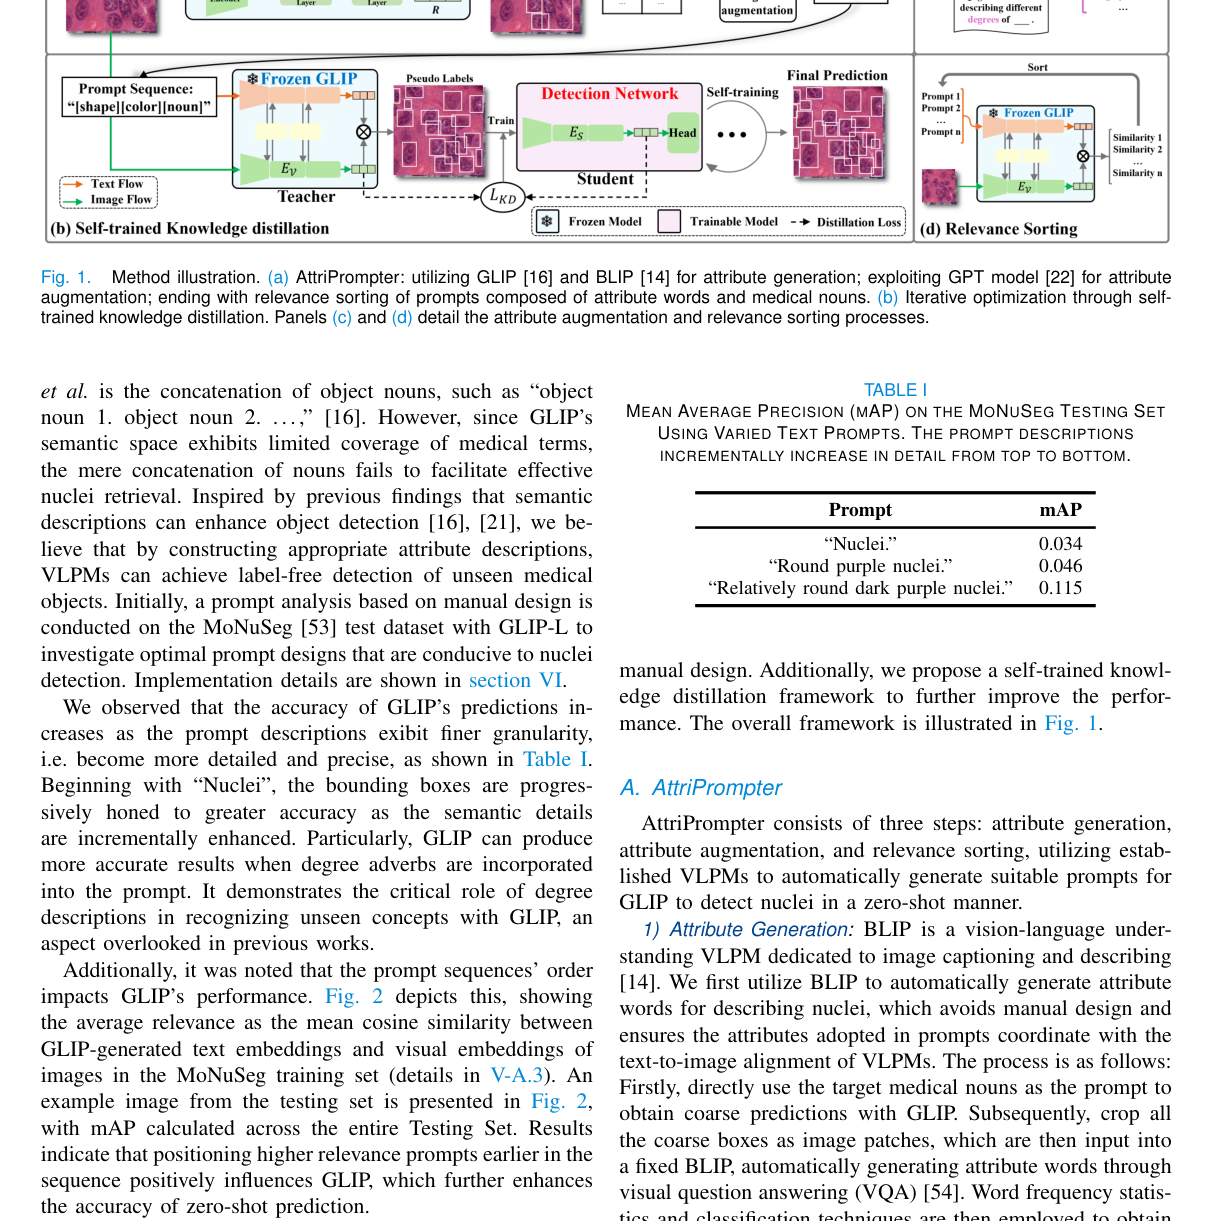
\includegraphics[width=0.92\textwidth]{figures/tmi_fig_method.png}
  \caption{第三章工作的补充框架图。该图以论文原始英文图为基础，在学位论文中可直接配合中文图题使用。}
\end{figure}

\begin{figure}[H]
  \centering
  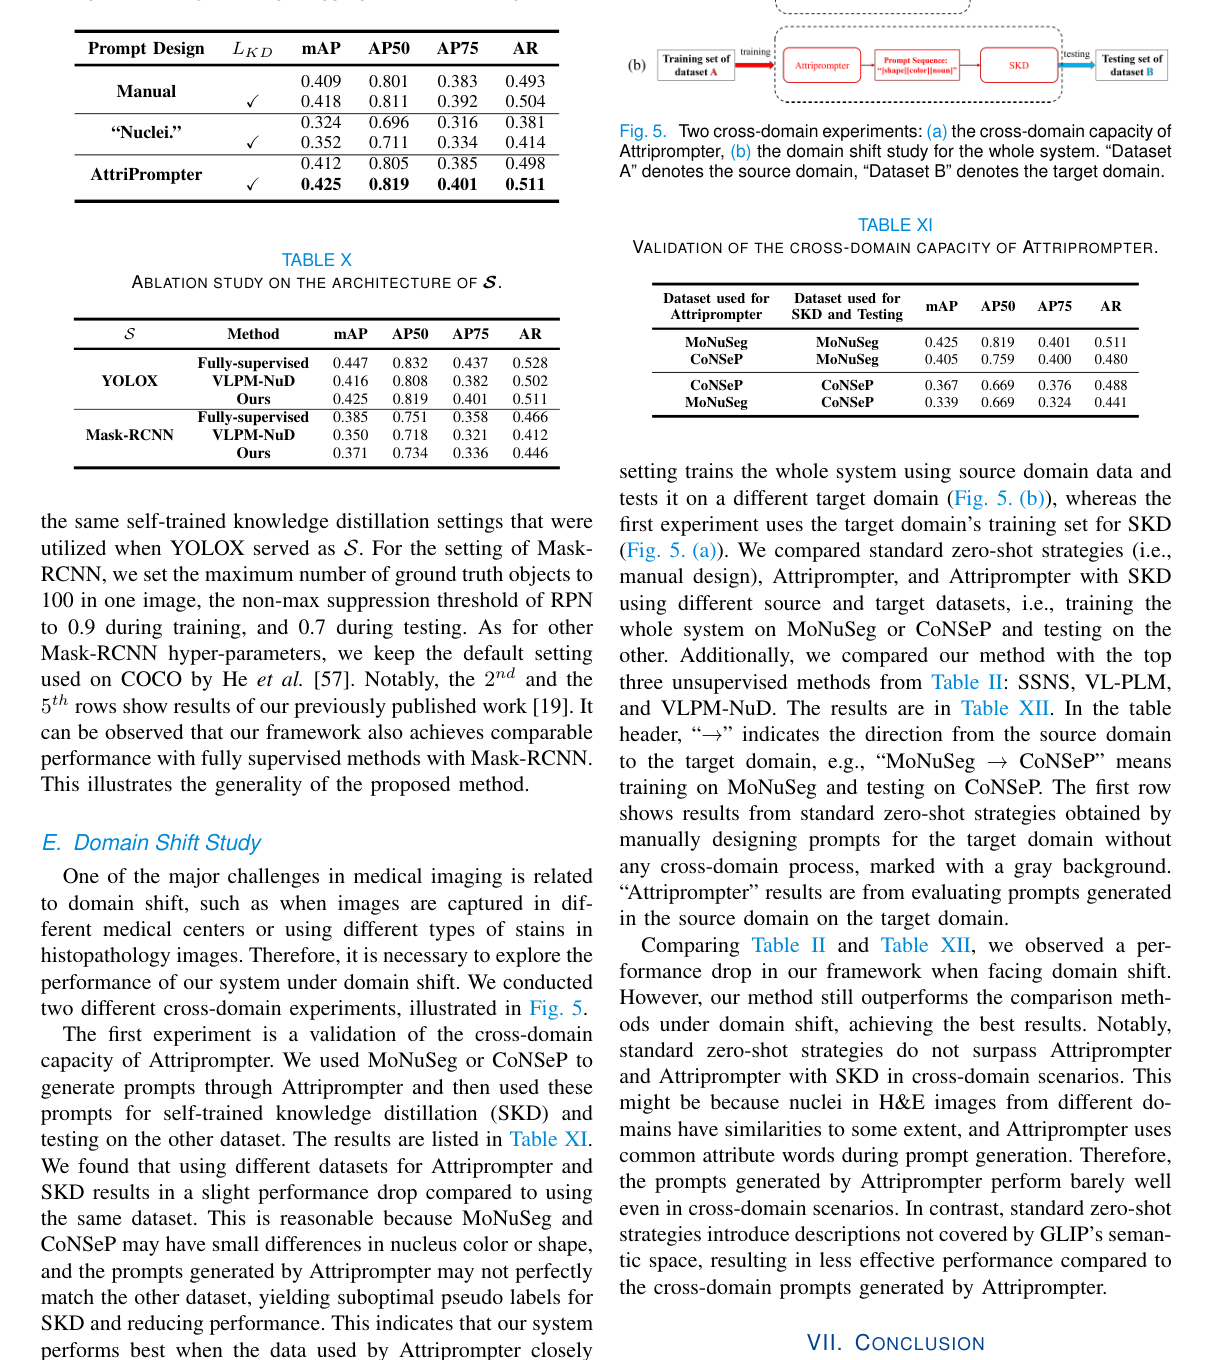
\includegraphics[width=0.92\textwidth]{figures/tmi_table_more_ablation.png}
  \caption{第三章工作的补充消融结果。通过增加该图，可以更充分地支撑属性解耦提示机制的有效性分析。}
\end{figure}

这些补充图表在学位论文中的作用不仅是“增加页数”，更重要的是让章节叙述与原始论文证据链形成紧密对应。特别是在答辩或导师审阅场景中，图表与正文一一对应，可以帮助读者快速理解该章的关键贡献点和实验支撑关系。

\section{第四章补充图表与讨论}
\begin{figure}[H]
  \centering
  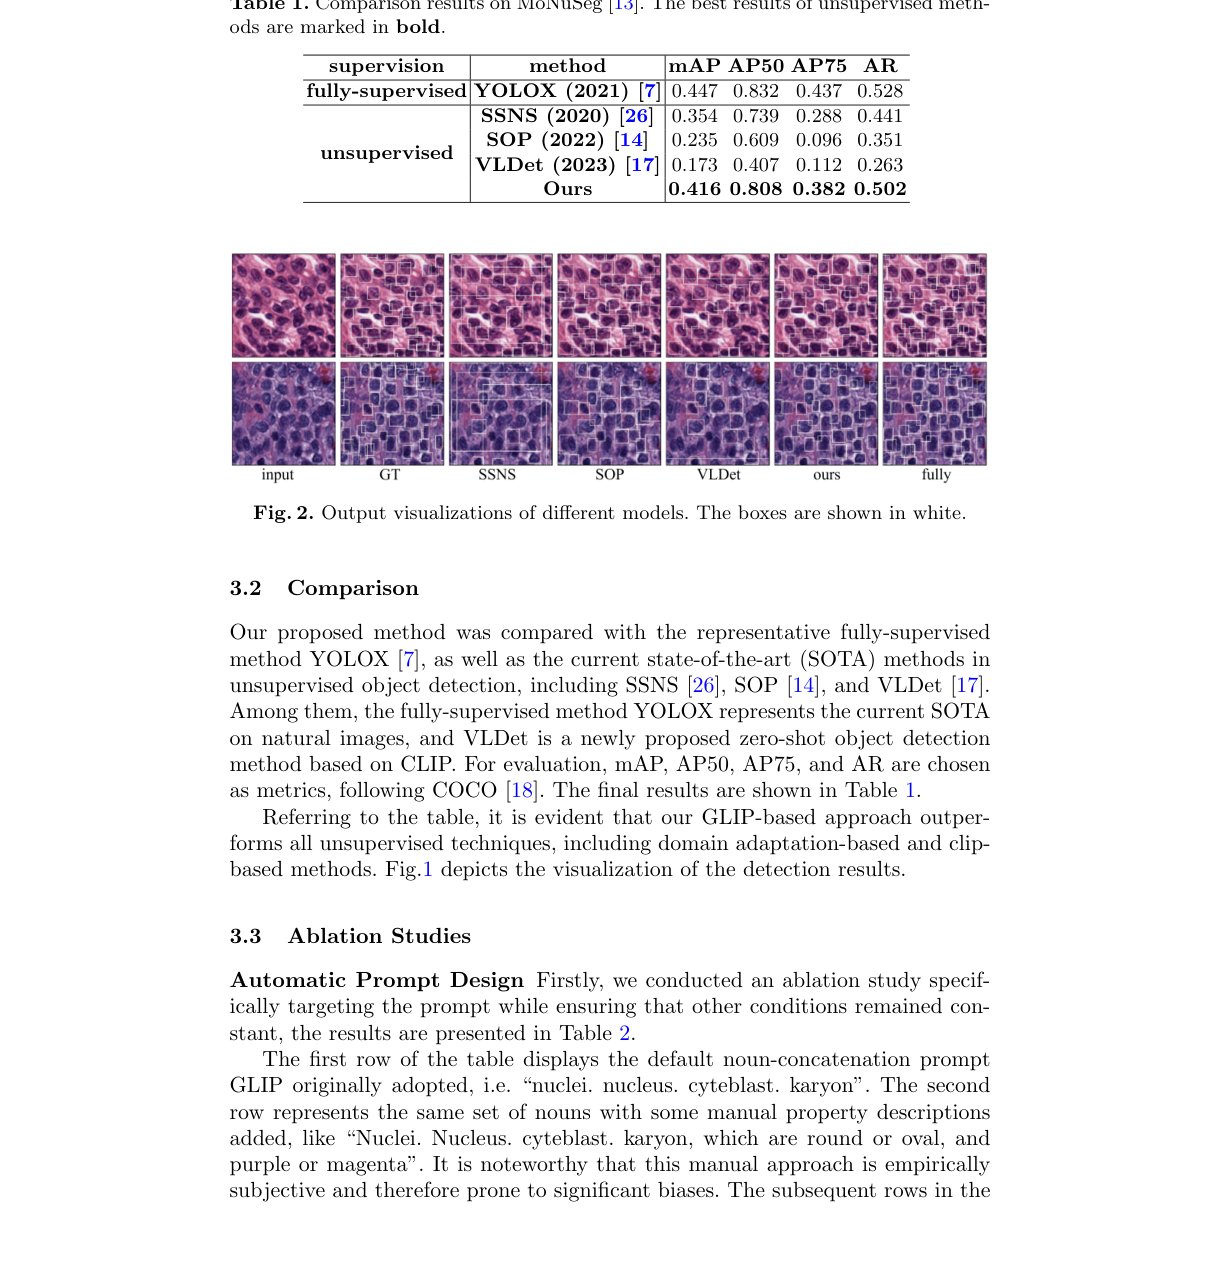
\includegraphics[width=0.9\textwidth]{figures/miccai_table_main.png}
  \caption{第四章主要检测结果补充图。由于原始论文以英文表格呈现，这里保留原图并辅以中文叙述，可较快扩充大论文章节内容。}
\end{figure}

\begin{figure}[H]
  \centering
  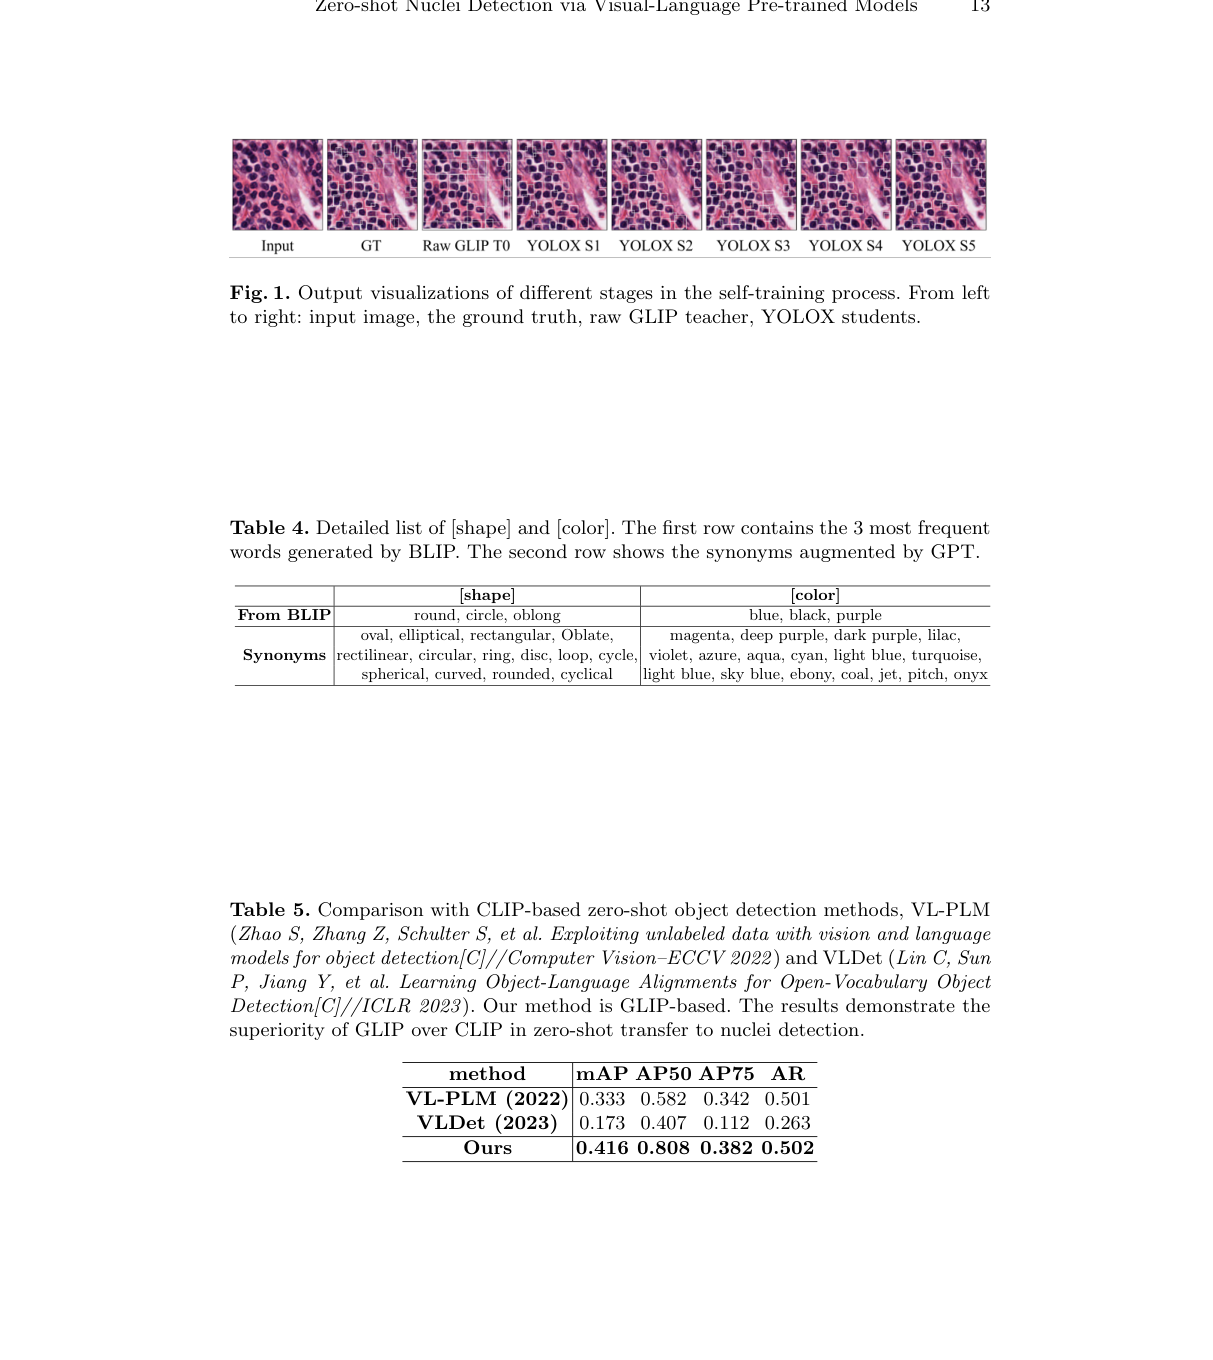
\includegraphics[width=0.9\textwidth]{figures/miccai_fig_selftrain.png}
  \caption{第四章自训练增益补充图。该图适合与正文中的“从零样本预测到目标域适配”的叙述相配合。}
\end{figure}

与第三章类似，第四章的补充图表强化了“自动属性提示 + 自训练”的双阶段逻辑。把这类图表单独置于附录，一方面可以避免主体章节过于拥挤，另一方面也能在审稿或送审版本中体现工作量与证据链的完整性。

\section{第五章补充图表与讨论}
\begin{figure}[H]
  \centering
  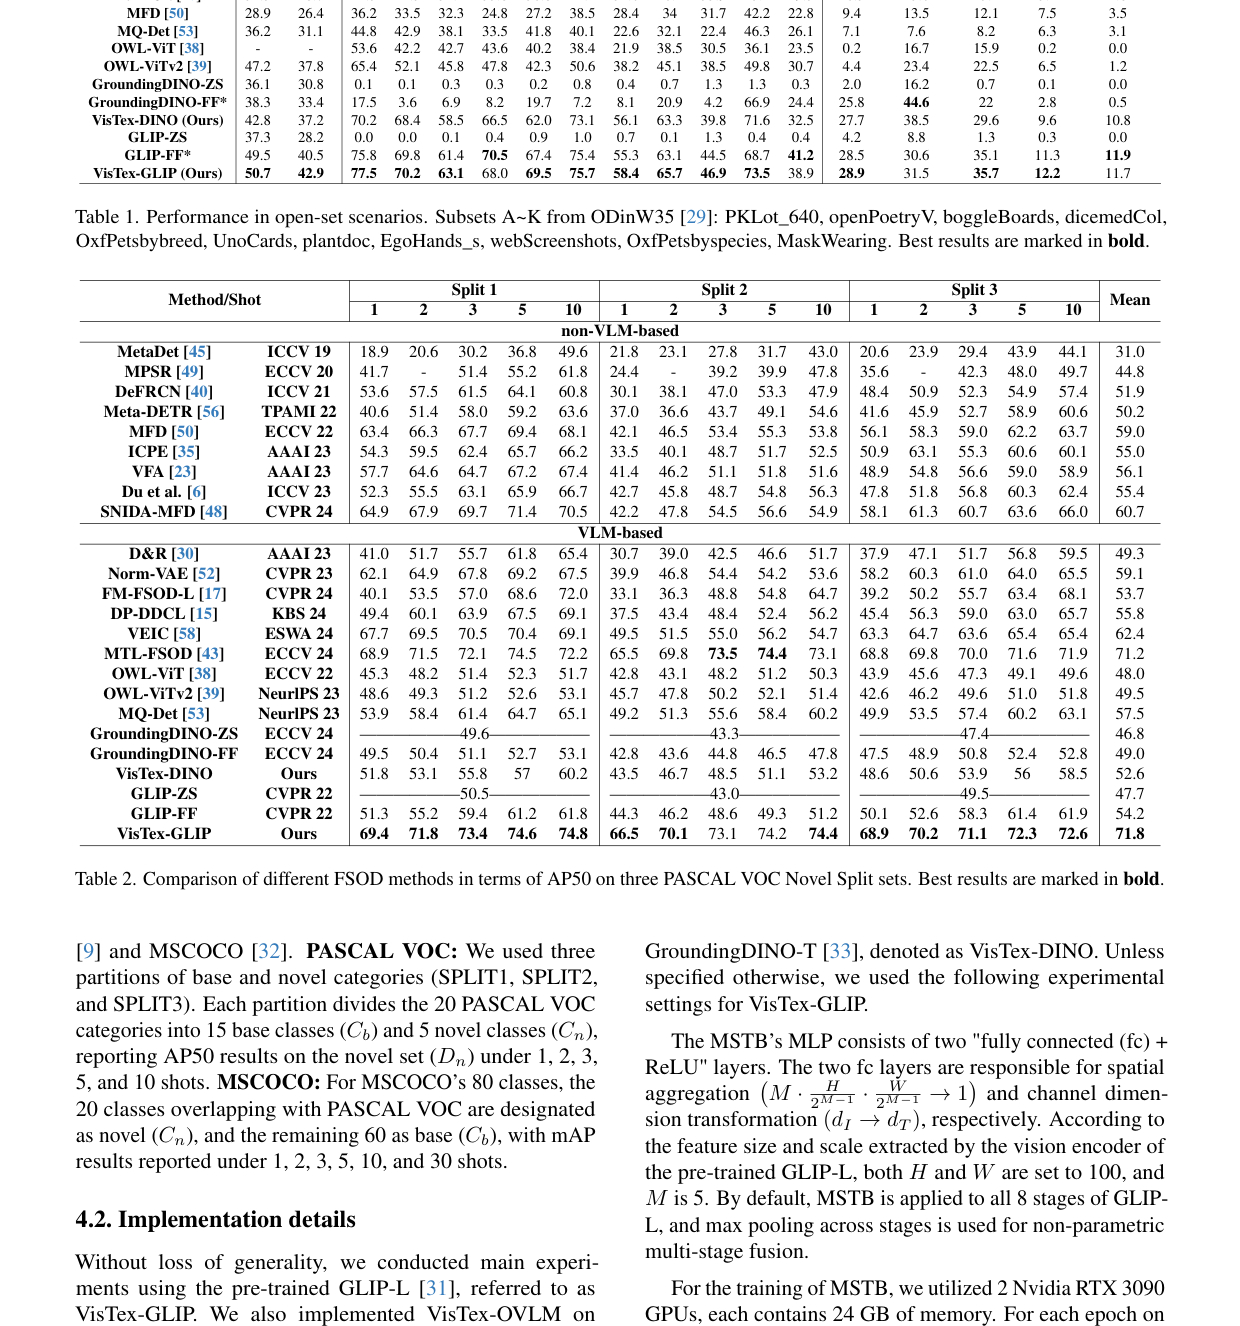
\includegraphics[width=\textwidth]{figures/vistex_table_main.png}
  \caption{第五章主要结果补充图。该图展示 VisTex 与多种基线方法在跨域提示任务中的总体比较。}
\end{figure}

\begin{figure}[H]
  \centering
  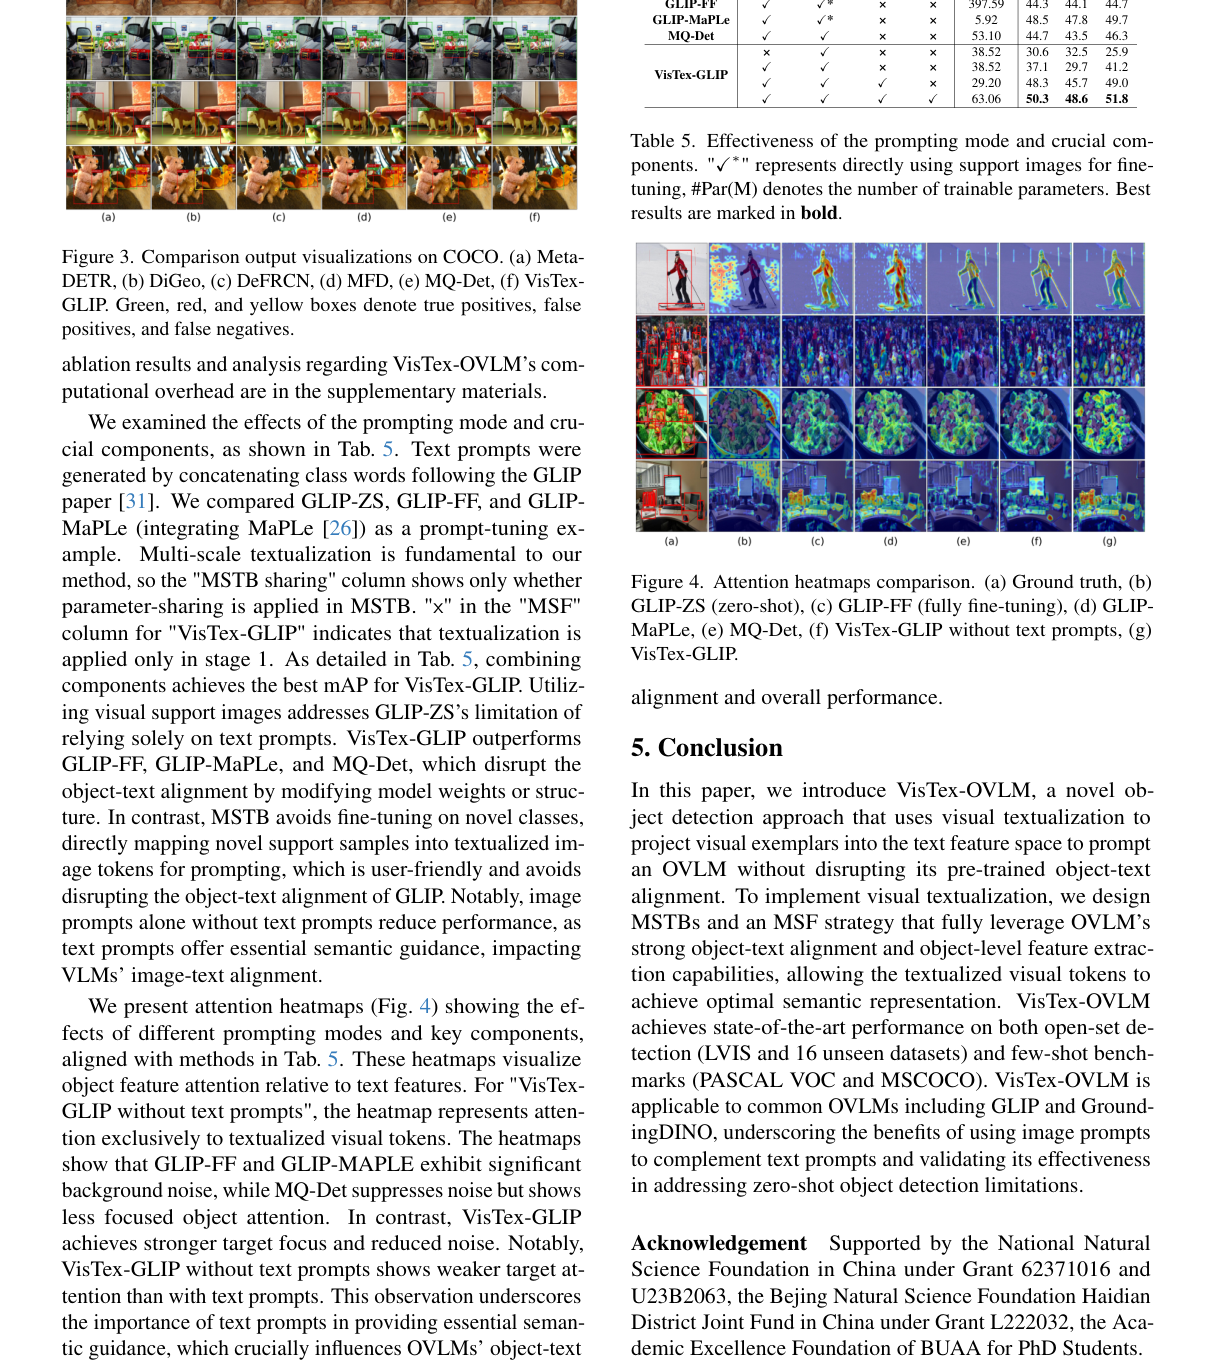
\includegraphics[width=\textwidth]{figures/vistex_fig_vis.png}
  \caption{第五章可视化案例补充图。该图有助于展示图像提示对困难样本的具体改善方式。}
\end{figure}

在大论文写作中，第五章往往最容易因为方法较新、概念较多而显得抽象。通过增加框架图、主结果表和可视化对比图，可以显著提升章节的可读性，使读者更容易理解“视觉文本化”究竟带来了什么。

\section{第六章补充图表与讨论}
\begin{figure}[H]
  \centering
  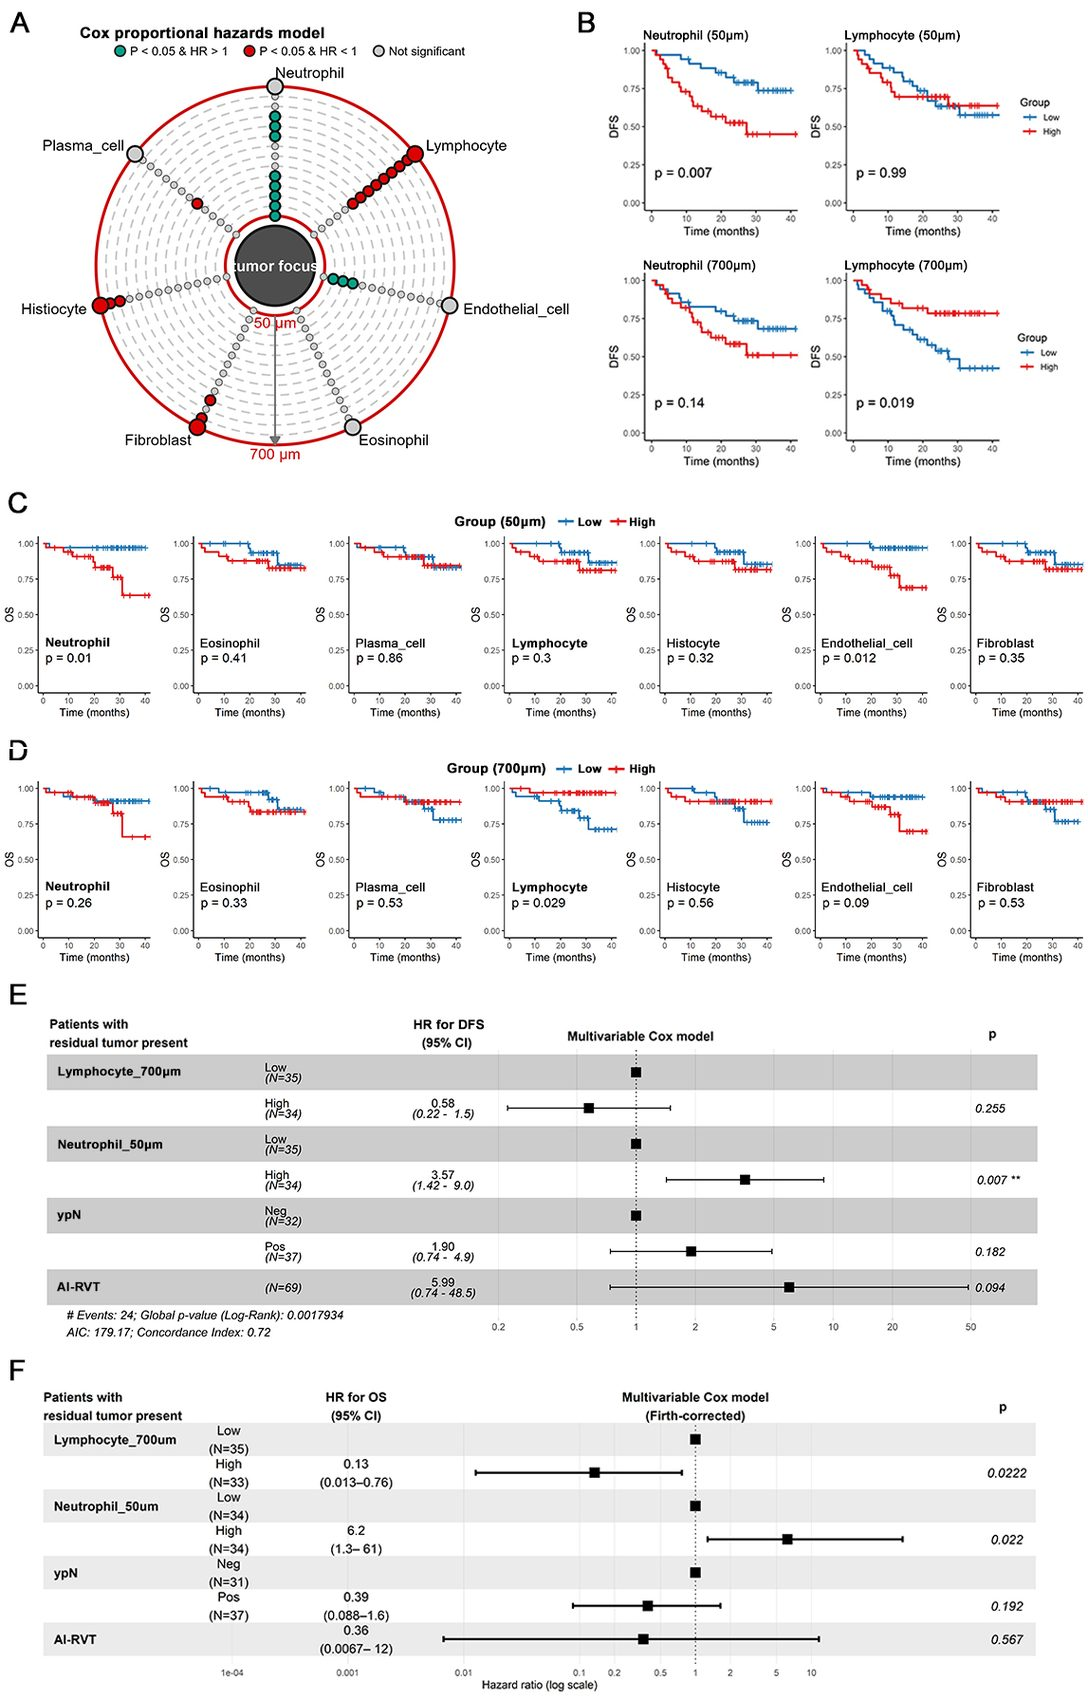
\includegraphics[width=\textwidth]{figures/lung_image5.jpeg}
  \caption{第六章生存分析补充图。将该类图表纳入学位论文附录，有助于增强临床分析部分的完整性。}
\end{figure}

\begin{figure}[H]
  \centering
  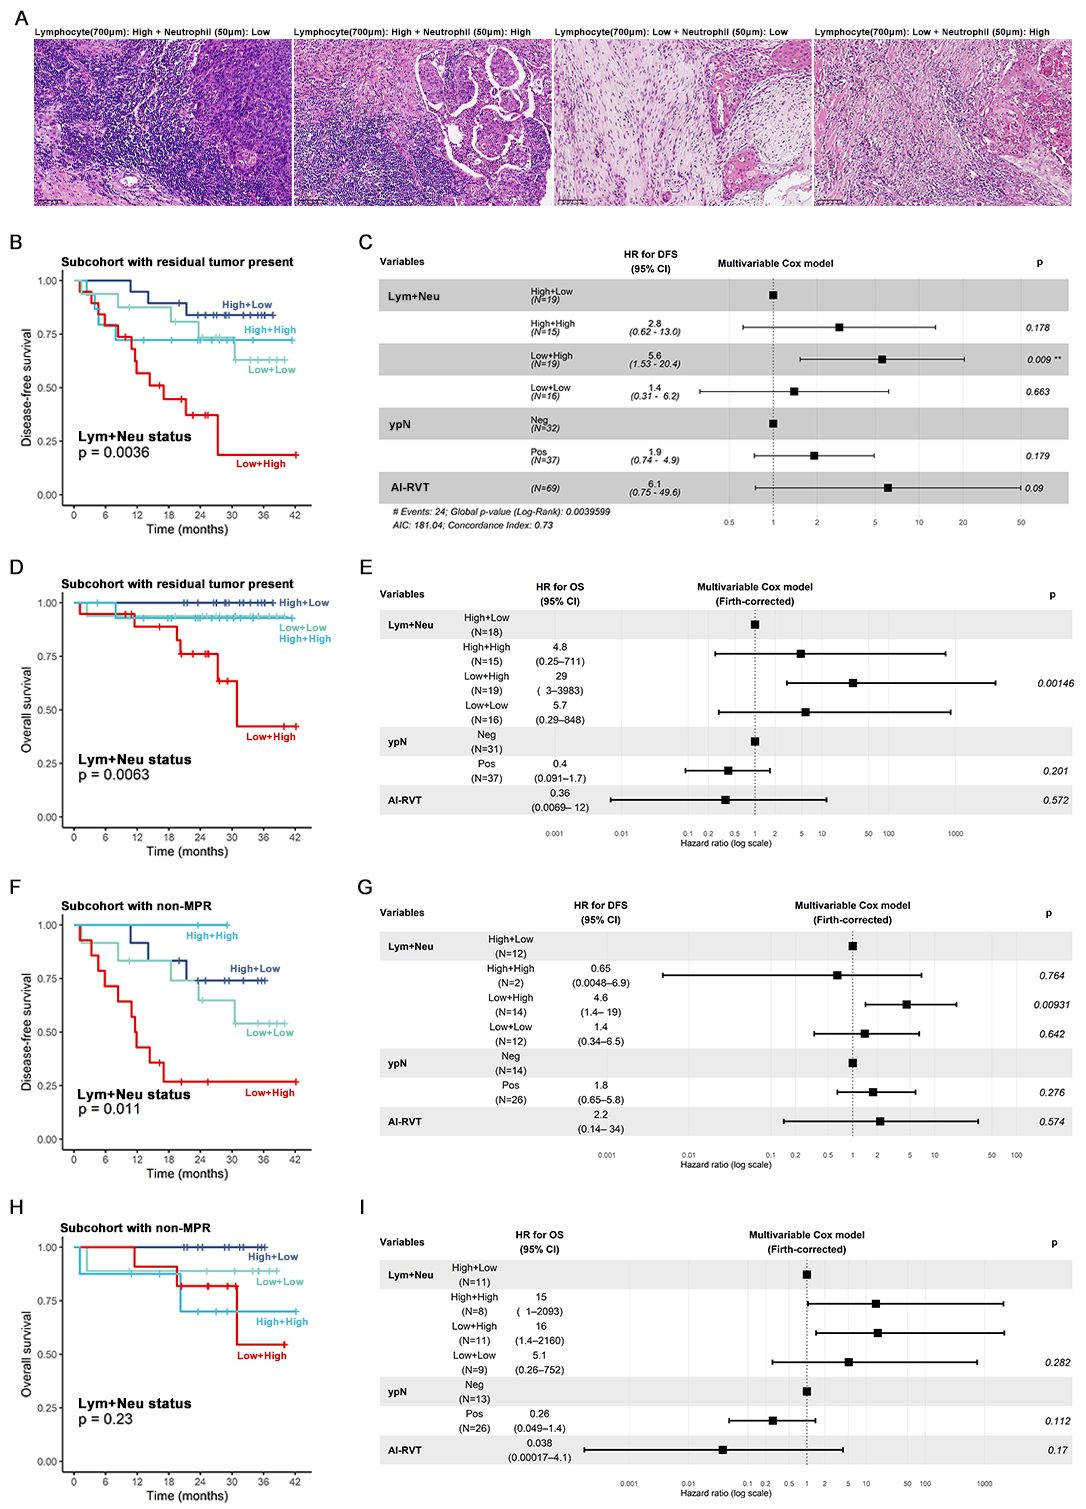
\includegraphics[width=\textwidth]{figures/lung_image6.jpeg}
  \caption{第六章亚组分析补充图。该图可用于说明数字病理指标在不同患者群体中的稳定性。}
\end{figure}

对于临床应用章节而言，图表的作用尤其突出。因为这类工作最终关注的是“指标是否具有临床解释性”，而临床解释性往往必须通过统计图、风险分层图和生存分析图来体现。把这部分材料系统纳入附录，也有助于后续把学位论文版本与在投论文版本进行更高效的互相映照。

\section{扩展讨论：如何把论文进一步扩充为送审版本}
如果后续仍需要把学位论文进一步扩展到更大体量，一个自然方向是把各章实验分析继续细分。例如，第三章可以单独增加“失败案例分析”和“不同属性分支作用的统计汇总”；第四章可以增加“提示模板的语义层次分析”和“自训练伪标签质量变化曲线”；第五章可以补充“直接测试与微调模式差异分析”；第六章则可以进一步增加病例来源、纳排标准、病理阅片流程以及更多临床协变量分析。

另一个适合扩写的部分是对相关工作的系统梳理。事实上，视觉语言预训练、提示学习、零样本检测、医学 few-shot 学习以及数字病理分析本身都已经形成相对成熟的研究脉络。在毕业论文中，把这些脉络系统梳理出来，不仅有助于增加篇幅，更重要的是能够明确本论文各章在整个研究版图中的定位。也就是说，增加附录和图表只是“做厚”的一种方式，而构建更完整的学术叙事则是让论文真正变得扎实的关键。

\let\chapter\savedchapter
}

\achievement

\begin{enumerate}[label=(\arabic*)]
  \item Wu, Y., Zhou, Y., Saiyin, J., Wei, B., Lai, M., Shou, J., et al. \emph{Dual-modal Vision-Language Prompting for Unseen Nuclei Instance Segmentation via Attribute Disentanglement}. IEEE Transactions on Medical Imaging.
  \item Wu, Y., Zhou, Y., Saiyin, J., Wei, B., Lai, M., Shou, J., et al. \emph{Zero-shot Nuclei Detection via Visual-Language Pre-trained Models}. MICCAI 2023.
  \item Wu, Y., Zhou, Y., Saiyin, J., Wei, B., Xu, Y. \emph{Visual Textualization for Image Prompted Object Detection}. ICCV 2025.
  \item \emph{AI-Based Assessment of Tumor Regression and Peritumoral Immune Cells Density Predicts Outcomes in Non-pCR Lung Squamous Cell Carcinoma Following Neoadjuvant Immunochemotherapy}. 在投.
\end{enumerate}

\acknowledgments

攻读博士学位期间，作者在导师和课题组成员的帮助下，围绕医学图像检测、分割、视觉语言预训练、提示学习以及数字病理分析开展了系统研究。感谢导师在科研选题、方法设计、论文写作和学术训练方面给予的长期指导，也感谢课题组同学在实验复现、结果讨论和论文修改过程中提供的帮助。

感谢合作单位和合作者在病理数据、医学知识、临床问题定义和结果解释方面给予的支持。医学人工智能研究离不开跨学科协作，本文涉及的细胞核检测、实例分割和肺鳞癌疗效评估工作，均受益于工程、医学和病理学团队之间的持续交流。

感谢家人和朋友在求学过程中的理解、支持与鼓励。未来，作者将继续围绕可信、低标注成本和可解释的医学人工智能方法开展研究，努力推动相关技术在真实临床场景中的应用。

\biography

吴永健，北京航空航天大学博士研究生，主要研究方向为医学图像分析、数字病理、视觉语言预训练模型与提示学习。攻读学位期间，围绕低标注成本医学图像检测与分割、零样本细胞核检测、图像提示目标检测与数字病理临床分析等问题开展研究，并形成多项相关学术成果。


\end{document}
